\documentclass[a4paper,openany]{book}
\usepackage{amssymb,amsthm,makeidx,enumerate}
\usepackage[utf8]{vietnam}
\usepackage{scrextend} %Tăng cỡ chữ
\changefontsizes{13pt}%Cỡ chữ mới là 13pt
\usepackage[top=2.5cm, bottom=2.5cm, left=2.0cm, right=2.0cm] {geometry}
\setlength{\parindent}{0.6cm}
\setlength{\parskip}{0.2cm}
\makeindex
\usepackage{amsmath}
\usepackage{amsfonts}
\usepackage{amssymb}
\usepackage{chngcntr}
\usepackage{graphicx}
\usepackage{glossaries}
\counterwithin{equation}{section} % cho công thức toán học
\usepackage{anyfontsize}
\usepackage{listings}
\makeatletter
\long\def\@makecaption#1#2{%
  \vskip\abovecaptionskip
    \bfseries #1: #2\par
  \vskip\belowcaptionskip}%
\makeatother
\usepackage{color}
\usepackage{graphicx}
\usepackage{subcaption}
%%%%%%%%%%%%%%%%%%%%%%%%%%%%%%%%%%%%%%%%%%%%%%%%%%%%%%%%%%%%%%%
%%%%%%%%%%%%%%%%%% Nhúng link vào trong phần \ref
%%%%%%%%%%%%%%%%%%%%%%%%%%%%%%%%%%%%%%%%%%%%%%%%%%%%%%%%%%%%%%%
\usepackage[unicode]{hyperref} %link

%%%%%%%%%%%%%%%%%%%%%%%%%%%%%%%%%%%%%%%%%%%%%%%%%%%%%%%%%%%%%%%
%%%%%%%%%%%%%%%%%% Đóng khung phần chứng minh thêm vào
%%%%%%%%%%%%%%%%%%%%%%%%%%%%%%%%%%%%%%%%%%%%%%%%%%%%%%%%%%%%%%%
\usepackage{tikz,lipsum,lmodern}
\usepackage[most]{tcolorbox}


%%%%%%%%%%%%%%%%%%%%%%%%%%%%%%%%%%%%%%%%%%%%%%%%%%%%%%%%%%%%%%%
%%%%%%%%%%%%%%%%%% Hiển thị code
%%%%%%%%%%%%%%%%%%%%%%%%%%%%%%%%%%%%%%%%%%%%%%%%%%%%%%%%%%%%%%%
\usepackage{xcolor}

\definecolor{codegreen}{rgb}{0,0.6,0}
\definecolor{codegray}{rgb}{0.5,0.5,0.5}
\definecolor{codepurple}{rgb}{0.58,0,0.82}
\definecolor{backcolour}{rgb}{0.95,0.95,0.92}

\lstdefinestyle{mystyle}{
    backgroundcolor=\color{backcolour},   
    commentstyle=\color{codegreen},
    keywordstyle=\color{magenta},
    numberstyle=\tiny\color{codegray},
    stringstyle=\color{codepurple},
    basicstyle=\ttfamily\footnotesize,
    breakatwhitespace=false,         
    breaklines=true,                 
    captionpos=b,                    
    keepspaces=true,                 
    numbers=left,                    
    numbersep=5pt,                  
    showspaces=false,                
    showstringspaces=false,
    showtabs=false,                  
    tabsize=2
}

\lstset{style=mystyle}


%%%%%%%%%%%%%%%%%%%%%%%%%%%%%%%%%%%%%%%%%%%%%%%%%%%%%%%%%%%%%%%
%%%%%%%%%%%%%%%%%% Đóng khung phần chứng minh thêm vào
%%%%%%%%%%%%%%%%%%%%%%%%%%%%%%%%%%%%%%%%%%%%%%%%%%%%%%%%%%%%%%%
\definecolor{dkgreen}{rgb}{0,0.6,0}
\definecolor{gray}{rgb}{0.5,0.5,0.5}
\definecolor{mauve}{rgb}{0.58,0,0.82}
\lstset{frame=tb,
	language=R,
	aboveskip=3mm,
	belowskip=3mm,
	showstringspaces=false,
	columns=flexible,
	basicstyle={\small\ttfamily},
	numbers=none,
	numberstyle=\tiny\color{gray},
	keywordstyle=\color{blue},
	commentstyle=\color{dkgreen},
	stringstyle=\color{mauve},
	breaklines=true,
	breakatwhitespace=true,
	tabsize=3
}
\begin{document}
\input def
\pagestyle{myplain}
\begin{titlepage}
%\thispagestyle{empty}
\begin{center}
{\bf  TRƯỜNG ĐẠI HỌC SƯ PHẠM TP. HỒ CHÍ MINH}\\
\hfill

\vspace*{2cm}

\begin{figure} [ht]
  \centering
  
\includegraphics[scale = 0.75]{image/Toan1.png}
\end{figure}
\vspace*{2cm}

{\huge\bf ƯỚC LƯỢNG ĐỆ QUY TRONG LỚP CÁC MÔ HÌNH BIẾN DẠNG}

\vspace*{3cm}
{\large\bf  ĐINH MINH HẢI}\\
{\large\bf  KHÓA LUẬN TỐT NGHIỆP}

\vfill

{\bf Tp. Hồ Chí Minh - 2024}
\end{center}
\end{titlepage}


\newpage
\thispagestyle{empty}
\begin{center}
{\bf  TRƯỜNG ĐẠI HỌC SƯ PHẠM TP. HỒ CHÍ MINH}\\


\vspace*{1.5cm}

{\bf  ĐINH MINH HẢI}

\vspace*{1.5cm}

{\huge\bf ƯỚC LƯỢNG ĐỆ QUY TRONG LỚP CÁC MÔ HÌNH BIẾN DẠNG}

\vspace*{1.5cm}

{\bf KHÓA LUẬN TỐT NGHIỆP}\\[20pt]
\end{center}
\vspace*{1.5cm}

{\fontsize{13}{1}\selectfont Ngành: Sư phạm Toán học} 

{\fontsize{13}{1}\selectfont Mã số ngành: 7140209}


\vspace*{3cm}

GIẢNG VIÊN HƯỚNG DẪN 

{\bf ThS. NGUYỄN PHÁT ĐẠT}

\vfill
\begin{center}
{\bf Tp. Hồ Chí Minh - 2024}
\end{center}



\addcontentsline{toc}{chapter}{Lời cam đoan}

%\vspace*{3cm}

\textbf{{\LARGE \begin{center}
			Lời cam đoan
\end{center}}}

%\vspace*{1cm}

\indent Tôi cam đoan khóa luận tốt nghiệp, với đề tài: "Ước lượng đệ quy trong lớp các mô hình biến dạng" là công trình khoa học do tôi - Đinh Minh Hải thực hiện dưới sự hướng dẫn của ThS. Nguyễn Phát Đạt.

Những kết quả được trình bày trong khóa luận là trung thực và chính xác.

\begin{flushright}
    Sinh viên thực hiện $ \qquad \quad $
	
	\vspace*{3cm}
	
	{\bf Đinh Minh Hải  $\quad \quad \quad$}
	
	
\end{flushright}


\thispagestyle{empty}
\begin{center}
\LARGE{\textbf{Lời cảm ơn}}
\end{center}
Em xin bày tỏ lòng biết ơn sâu sắc đến thầy Nguyễn Phát Đạt, người đã hướng dẫn tận tâm giúp em hoàn thành khóa luận này. Sự nhiệt tình của thầy luôn tạo động lực cho em vượt qua mọi khó khăn trong nghiên cứu và thực hiện khóa luận. Xin cảm ơn triết lý học võ tự vệ của người làm xác suất mà thầy có dịp thảo luận với sinh viên, nó thực sự rất hay.

Em cũng xin gửi lời cảm ơn chân thành đến các thầy cô trong tổ Toán Ứng dụng đã tạo điều kiện và hỗ trợ em trong suốt quá trình nghiên cứu và thực hiện khóa luận.

Xin cảm ơn thầy Đào Huy Cường vì một học phần "Xác suất thống kê" vô cùng hay và ý nghĩa, đã đưa em từng bước từng bước, xây dựng nên tảng kiến thức cho các học phần khác về xác suất sau này mà cuối cùng là khóa luận tốt nghiệp.

Xin cảm ơn thầy Nguyễn Thành Nhân cho những triết lý học tập vô cùng sâu sắc mà thầy truyền đạt trong học phần "Giải tích hàm nhiều biến". Em luôn ghi nhớ những câu chuyện và những hướng dẫn của thầy về cách học, cách chuẩn bị cho các kỳ thi và chuẩn bị cho tương lai dài hạn từ một thời điểm rất lâu trước đó. Đặc biệt, em sẽ luôn ghi nhớ tháp tam giác phân loại những người làm toán và sự khiêm tốn của thầy khi nói về chỗ mà thầy đứng trong tháp tam giác đó. 

Xin cảm ơn thầy Phạm Duy Khánh cho những tiết học chặt chẽ về toán ở học phần "Lý thuyết tối ưu" và sự nghiêm túc của thầy trong học tập và làm việc nhưng vô cùng thoải mái ngoài đời. Em quý thầy nhưng cũng rất rén khi gặp thầy.

Xin cảm ơn bố mẹ tôi, bố Thêm, mẹ Hường đã nuôi dưỡng tôi nên người và lo lắng cho tôi trong suốt năm tháng học tập ở trường Đại học Sư phạm. 

Xin cảm ơn anh trai tôi - Minh Hoàng vì sự có mặt của anh trong suốt thời thơ ấu và trong nền giáo dục gian truân mà khắc khổ từ gia đình dành cho chúng tôi. Mong anh có thể đi những bước vững chãi trong cuộc sống của anh.

Xin cảm ơn vợ tôi - Gia Hân đã luôn động viên tinh thần và tiếp tế nguồn lực cho tôi trong suốt những ngày làm khóa luận khó khăn. Cảm ơn em cho những góp ý sâu sắc về những điều cần phải làm trong các vấn đề bên lề của khóa luận này. Cảm ơn em vì phần đồ ăn chuẩn bị cho năm ngày làm việc liên tục để hoàn thành khóa luận này.

Xin cảm ơn người bạn lâu năm - Minh Đức đã đánh cờ giải lao với tôi sau những lần chứng minh định lý, và những giờ bơi đua rất tốn thể lực nhưng đầy sảng khoái mỗi tuần.

Xin cảm ơn Tấn Phát và Giáp Thân đã chinh chiến cùng tôi trên sân chơi Olympic Tin học sinh viên. Thời gian đó thực sự là một bước ngoặt về chất để tôi chuẩn bị cho sự mài dũa tư duy cá nhân, tư duy học toán thông qua việc viết, trình bày và giải rất nhiều ra nháp, đồng thời là cả tư duy về lập trình thuật toán - điều giúp ích cho tôi rất nhiều khi viết những dòng code để ước lượng hàm hồi quy.

Xin cảm ơn Uyên Phương vì những hỗ trợ của Phương trong kỳ Thực tập Sư phạm 2 và những chia sẻ của Phương về tinh thần học tập và làm việc nghiêm túc. Xin cảm ơn tinh thần lạc quan và hoan hỉ Phương trong mọi khó khăn của công việc.

Xin cảm ơn Như Ý, Anh Tuấn vì những thiện ý khi nhóm chúng ta làm việc cùng nhau.

Xin cảm ơn anh Quân vì những câu chuyện bên lề khóa luận dở khóc dở cười.

Xin cảm ơn các thầy, các cô ở trường Đại học Sư phạm mà tôi may mắn có dịp học cùng. Các thầy các cô là tấm gương rực rỡ để chúng em học hỏi và phát triển sự nghiệp toán học của riêng mình. Xin cảm ơn các thầy cô rất nhiều.

Lời cuối cùng, xin cảm ơn những đọc giả đã hoan hỉ cùng tôi bước qua rất nhiều những lời cảm ơn bên trên. Tôi không mong các bạn thấy mệt mỏi vì nó thể hiện quá trình học ở trường Sư Phạm đầy ý nghĩa và nhiều màu sắc của tôi ở đây. Và một lý do khác nữa là chúng ta cần lên dây cót tinh thần để bước vào nội dung chính của tài liệu này: khóa luận tốt nghiệp của tôi - Đinh Minh Hải.

\begin{flushright}
{\it Tp.HCM, ngày 03 tháng 05 năm 2023}

Tác giả\hskip 2cm\quad

\vskip 2cm

{\bf Đinh Minh Hải} $\;\;\;\;\;\;\;$ \hskip 1cm 
 \end{flushright}
\thispagestyle{empty}

\tableofcontents
\addcontentsline{toc}{chapter}{Chú thích thuật ngữ}
\chapter*{Chú thích thuật ngữ}
\textbf{Biến phân bình phương (hoặc đặc trưng bình phương) dự báo được}: Predictable variation.\\
\textbf{Bộ lọc}: Filtration.\\
\textbf{Dãy tin cậy}: Confidence band.\\
\textbf{Dữ liệu có chu kỳ (hoặc dữ liệu tuần hoàn)}: Periodic data.\\
\textbf{Mô hình biến dạng}: Deformation model.\\
\textbf{Mô hình biến dạng theo chu kỳ (hoặc mô hình bất biến dáng điệu)}: Shape-Invariant Model.\\
\textbf{Tính chặt/bị chặn theo xác suất}: Tightness.\\
\textbf{Tham số chiều cao}: Height parameter.\\
\textbf{Tham số chuyển đổi}: Translation parameter.\\
\textbf{Tham số co giãn}: Scale parameter.\\
\textbf{Trọng số tối ưu}: Optimal weight.\\
\textbf{Tương thích}: Adapted.\\
\textbf{Ước lượng đệ quy}: Recursive estimation.\\




% \addcontentsline{toc}{chapter}{Trang thông tin Sản phẩm nghiên cứu khoa học}

% \textbf{{\Large \begin{center}
% 			TRANG THÔNG TIN SẢN PHẨM 
% \end{center}}}

% Tên đề tài: \textbf{ABC XYZ.}

% Chuyên ngành: c.

% Mã số ngành: xxyyzz.

% Tên nhóm cá sinh viên thực hiện: .

% Khóa đào tạo: .

% Người hướng dẫn khoa học: ThS Nguyễn Phát Đạt.

% Cơ sở đào tạo: .

% {\bf 1. TÓM TẮT NỘI DUNG SẢN PHẨM NGHIÊN CỨU KHOA HỌC:}


% \begin{description}
% 	\item [Chương 1:] . 
% 	\item [Chương 2:] .
% 	\item[Chương 3:].
	
% 	\item[Chương 4:] .
	
% \end{description}


% {\bf 2. NHỮNG KẾT QUẢ MỚI:} Không có.


% {\bf 3. CÁC ỨNG DỤNG/ KHẢ NĂNG ỨNG DỤNG TRONG THỰC TIỄN HAY NHỮNG VẤN ĐỀ CÒN BỎ NGỎ CẦN TIẾP TỤC NGHIÊN CỨU}.\\





% {\bf TẬP THỂ CÁN BỘ HƯỚNG DẪN} $ \qquad \qquad  $ {\bf SINH VIÊN}

% $ \qquad \qquad $ (Ký tên, họ tên) $ \qquad \qquad \qquad \qquad \qquad \qquad \quad $ (Ký tên, họ tên)

% \vspace*{2cm}

% $\qquad \quad$ \textbf{NGUYỄN PHÁT ĐẠT} $ \qquad \qquad \qquad \quad \quad \quad$ \textbf{ĐINH MINH HẢI}

% \vspace*{0.2cm}



% \vspace*{0.2cm}

% \begin{center}
% 	{\bf XÁC NHẬN CỦA CƠ SỞ ĐÀO TẠO}\\
% {\bf HIỆU TRƯỞNG}
% \end{center}


\chapter*{Lời nói đầu}
\addcontentsline{toc}{chapter}{Lời nói đầu}

Các phân tích thống kê những mô hình gắn với dữ liệu có chu kỳ cung cấp cho chúng ta một phép xấp xỉ đủ tốt để mô phỏng các hiện tượng tự nhiên. Ví dụ như mô hình mô hình biến dạng theo chu kỳ có tham số chuyển và hàm hồi quy chưa biết trong bài báo \cite{bercu} có thể dùng để mô phỏng tín hiệu điện tim ở người khỏe mạnh hoặc ở người bị loạn nhịp tim. Tuy nhiên, mô hình trong bài báo năm 2012 này được thiết kế với một biến đầu vào nên cần mở rộng các kết quả đã đạt được lên mô hình nhiều biến và bổ sung các tham số quan trọng khác như chiều cao và co giãn chưa được đề cập, cùng với các ước lượng, sự hội tụ và tính tiệm cận chuẩn của chúng. Từ những lý do trên, khóa luận sẽ tập trung nghiên cứu các mô hình biến dạng nhiều biến có tham số chuyển, tham số chiều cao, co giãn và hàm hồi quy chưa biết trước.

Các mô hình biến dạng theo chu kỳ là các mô hình hồi quy bán tham số với một hàm tuần hoàn chưa biết. Xét các tập dữ liệu có liên quan đến hàm tuần hoàn và khác nhau ở ba tham số, một tham số chuyển, một tham số chiều cao và một tham số co giãn. Cụ thể mô hình trên được biểu diễn như sau
\begin{align}
    Y_{i, j}=a_{j} f\left(X_{i}-\theta_{j}\right)+v_{j}+\varepsilon_{i, j},
    \label{1.1}
\end{align}
trong đó $1 \leq j \leq p$ và $1 \leq i \leq n$, hàm dạng $f$ có chu kỳ và các $X_{i}$ là biến ngẫu nhiên, độc lập cùng phân phối.

Với $p=1, a_{1}=1$ và $v_{1}=0$, Bercu và Fraysse \cite{bercu} đề xuất một phương pháp đệ quy để ước lượng tham số chuyển $\theta_{1}$. Trong khóa luận này, tôi xin trình bày chi tiết các mở rộng của Fraysse [1] nhằm ước lượng tham số chiều cao $v$, tham số chuyển $\theta$ và tham số co giãn với số chiều $p$ tùy ý cho bởi
\begin{align}
    v=\left(\begin{array}{c}
v_{1} \\
\vdots \\
v_{p}
\end{array}\right), \quad \theta=\left(\begin{array}{c}
\theta_{1} \\
\vdots \\
\theta_{p}
\end{array}\right), \quad a=\left(\begin{array}{c}
a_{1} \\
\vdots \\
a_{p}
\end{array}\right).
\label{1.2}
\end{align}

Đầu tiên ta sẽ ước lượng vector tham số chiều cao $v$ bằng cách thiết lập một ước lượng vững tự nhiên $\widehat{v}_n$ hội tụ về $v$ và thiết lập tính tiệm cận chuẩn dựa trên định lý giá trị trung tâm cho martingales.

Sau đó, ta tiếp tục ước lượng tham số chuyển $\theta$ bằng thuật toán Robbins - Monro nhiều chiều với giả định rằng tồn tại một hàm $\phi: \mathbb{R}^{p} \rightarrow \mathbb{R}^{p}$, không chịu ảnh hưởng bởi $\theta$, sao cho $\phi(\theta)=0$. Khi đó 
\begin{align}
    \widehat{\theta}_{n+1}=\widehat{\theta}_{n}+\gamma_{n} T_{n+1},
    \label{1.3}
\end{align}
trong đó $\left(\gamma_{n}\right)$ là một dãy các số thực dương giảm dần về 0 và dãy $\left(T_{n}\right)$ là dãy các vector ngẫu nhiên sao cho $\mathbb{E}\left[T_{n+1} \mid \mathcal{F}_{n}\right]=\phi\left(\widehat{\theta}_{n}\right)$ trong đó $\mathcal{F}_{n}$ là $\sigma$-đại số các biến cố đã xảy ra đến thời điểm thứ $n$. Dưới các điều kiện chuẩn trên hàm $\phi$ và trên dãy $\left(\gamma_{n}\right)$, một kết quả quan trọng trong \cite{bercu} là $\widehat{\theta}_{n}$ tiến về $\theta$ hầu chắc chắn. Tính tiệm cận chuẩn của $\widehat{\theta}_{n}$ có thể được tìm thấy trong \cite{pelletier_weak_convergence} trong khi luật mạnh dạng toàn phương và luật loga-lặp được thiết lập trong \cite{pelletier_on_the_almost}.\\
Tiếp đó, ta ước lượng tham số co giãn $a$ qua một ước lượng vững mạnh sử dụng ước lượng tiên nghiệm $\theta$. Cuối cùng là chứng minh chặt chẽ cách sử dụng ước lượng đệ quy Nadaraya-Watson có trọng \cite{duflo} nhằm ước lượng hàm hồi quy $f$. Việc này có sử dụng thêm các ước lượng trước đó cho $v, \theta$ và $a$, tương ứng với $\widehat{v}_{n}$, $\widehat{\theta}_{n}$ và $\widehat{a}_{n}$. Với mọi $x \in \mathbb{R}$, ước lượng của hàm $f$ xác định bởi
\begin{align}
    \widehat{f}_{n}(x)=\sum_{j=1}^{p} \omega_{j}(x) \widehat{f}_{n, j}(x)
    \label{1.4}
\end{align}
với 
$$
\widehat{f}_{n, j}(x)=\frac{1}{\widehat{a}_{n, j}} \frac{\sum_{i=1}^{n} W_{i, j}(x)\left(Y_{i, j}-\widehat{v}_{i-1, j}\right)}{\sum_{i=1}^{n} W_{i, j}(x)}
$$
và
$$
W_{n, j}(x)=\frac{1}{h_{n}} K\left(\frac{X_{n}-\widehat{\theta}_{n-1, j}-x}{h_{n}}\right),
$$
trong đó $\widehat{v}_{n, j}, \widehat{\theta}_{n-1, j}$ và $\widehat{a}_{n, j}$ tương ứng với thành phần thứ $j$ của $\widehat{v}_{n}, \widehat{\theta}_{n-1}$ và $\widehat{a}_{n}$. Hơn nữa, hạt nhân $K$ là một hàm mật độ được chọn trước và băng tần $\left(h_{n}\right)$ là một dãy các số thực dương giảm về 0.

Toàn bộ khóa luận cấu trúc thành 4 chương. Chương 1 trình bày mô hình và các giả thuyết cần thiết để thực hiện quá trình phân tích thống kê. Chương 2 là các kiến thức chuẩn bị trước khi đi vào chứng minh ở chương 3 dành cho việc ước lượng tham số của vector $v$, thuật toán Robbins-Monro cho việc các ước lượng tham số  $\theta$ và ước lượng tham số cho vector tham số co giãn $a$. Trong ba nội dung này, khóa luận trình bày chi tiết các chứng minh để thiết lập sự hội tụ hầu chắc chắn của $\widehat{v}_{n}, \widehat{\theta}_{n}$ và $\widehat{a}_{n}$ cùng với tính tiệm cận chuẩn của chúng. Luật mạnh dạng toàn phương cũng được cung cấp cho ba ước lượng này. Ngoài ra, phần cuối của chương 3 giải quyết vấn đề ước lượng phi tham số của hàm $f$. Dưới các giả định tiêu chuẩn thông thường trên hạt nhân $K$, ta sẽ chứng minh hội tụ từng điểm hầu chắc chắn của $\widehat{f}_{n}$ về hàm $f$ và tính tiệm cận chuẩn của $\widehat{f}_{n}$. Hơn nữa, các ràng buộc cho sự xác định duy nhất liên quan đến mô hình. Chương 4 bao gồm các thí nghiệm trên số liệu mô phỏng bằng ngôn ngữ lập trình R, minh họa cho hiệu năng của quy trình ước lượng bán tham số. Cuối cùng, là các kết luận, định hướng nghiên cứu trong tương lai, phụ lục và tài liệu tham khảo cho khóa luận.

\chapter{Giới thiệu mô hình và các giả thiết}
Ta sẽ tập trung vào mô hình, với \(1 \leq j \leq p\), trong đó \(p \geq 2\), và \(1 \leq i \leq n\)

\[ Y_{i, j}=a_{j} f\left(X_{i}-\theta_{j}\right)+v_{j}+\varepsilon_{i, j} , \]
trong đó, với mọi \(1 \leq j \leq p, a_{j} \neq 0\). Với mọi \(1 \leq i \leq n\), nhiễu \(\left(\varepsilon_{i, j}\right)\) là một dãy các biến ngẫu nhiên độc lập với giá trị trung bình bằng không và phương sai \(\mathbb{E}\left[\varepsilon_{i, j}^{2}\right]=\sigma_{j}^{2}\), và độc lập với các biến ngẫu nhiên \(X_{i}, i=\overline{1,n}\),. Ngoài ra, như trong \cite{bercu}, ta cần các giả thiết sau.

$\left(\mathcal{H}_{1}\right)$ Các quan trắc $\left(X_{i}\right)$ là độc lập, cùng phân phối với hàm mật độ $g$, dương trên giá của nó $[-1 / 2 ; 1 / 2]$. Hơn nữa, $g$ liên tục trên $\mathbb{R}$, khả vi cấp 2 với đạo hàm bị chặn.

$\left(\mathcal{H}_{2}\right)$ Hàm dạng \(f\) là hàm đối xứng, bị chặn, tuần hoàn với chu kỳ 1.

Ta tạm thời chấp nhận rằng mô hình biến dạng theo chu kỳ \ref{1.1} có thể xác định được với cách lựa chọn giả thuyết $\left(\mathcal{H}_{3}\right)$ và $\left(\mathcal{H}_{3}\right)$ sau đây. 

$
\begin{aligned}
& \left(\mathcal{H}_{3}\right) \quad \int_{-1 / 2}^{1 / 2} f(x) d x=0 , \\
& \left(\mathcal{H}_{4}\right) \quad a_{1}=1, \theta_{1}=0 \text { và } \max _{1 \leq j \leq p}\left|\theta_{j}\right|<1 / 4 .
\end{aligned}
$

Nói theo cách khác là tồn tại duy nhất ước lượng các tham số \(a, \theta, v\) cũng như là hàm dạng \(f\) với điều kiện $\left(\mathcal{H}_{3}\right)$ và $\left(\mathcal{H}_{4}\right)$ đúng. Điều này sẽ được làm rõ trong phần cuối cùng của chương 4.



\chapter{Kiến thức chuẩn bị}
%%%%%%%%%%%%%%%%%%%%%%%%%%%%%%%%%%%%%%%%%%%%%%%%%%%%%%%%%%%%%%%%%%
%%%%%%%%%%%%%% Kỳ vọng có điều kiện
%%%%%%%%%%%%%%%%%%%%%%%%%%%%%%%%%%%%%%%%%%5%%%%%%%%%%%%%%%%%%%%%%%
\section{Kỳ vọng có điều kiện và Martingale}
\subsection{Kỳ vọng có điều kiện}
{\dn Cho $\mathbf{X}: \Omega \rightarrow \mathbb{R}^{n}$ là một vector ngẫu nhiên được định nghĩa trên không gian xác suất $(\Omega, \mathcal{A}, \mathbb{P})$. Ánh xạ chiếu $\pi_{i}: \mathbb{R}^{n} \rightarrow \mathbb{R}$ của vector $n$ chiều $X$ lên thành phần thứ $i$ của nó, $X_{i}=\pi_{i}(\mathbf{X})$, là một hàm đo được Borel. Dẫn đến $X_{i}=\pi_{i} \circ \mathbf{X}$ là một biến ngẫu nhiên đối với mỗi $i \in \overline{1,n}$. Hơn nữa, không gian biến cố được sinh bởi vector ngẫu nhiên $\mathbf{X}$ được cho bởi
$$
\sigma(\mathbf{X})=\sigma\left(X_{1}, \ldots, X_{n}\right) .
$$}
\subsubsection{Kỳ vọng có điều kiện của biến ngẫu nhiên}
\quad Giả sử $\mathcal{F}$ là $\sigma$-đại số con của $\sigma$-đại  $\mathcal{A}$.
    Kỳ vọng có điều kiện của biến ngẫu nhiên $X \geq 0$ đối với $\mathcal{F}$ là biến ngẫu nhiên suy rộng không âm
\[
\mathbb{E}(X \mid \mathcal{F}): \Omega \rightarrow[0, \infty]
\]
sao cho

(i) $\mathbb{E}(X \mid \mathcal{F})$ là $\mathcal{F}$-đo được,

(ii) với mọi $A \in \mathcal{F}$
\[
\int_A X \, d\mathbb{P} = \int_A \mathbb{E}(X \mid \mathcal{F}) \, d\mathbb{P} .
\]

Giả sử $X$ là biến ngẫu nhiên bất kỳ sao cho với xác suất một
\[
\min \left\{\mathbb{E}\left(X^{+} \mid \mathcal{F}\right), \mathbb{E}\left(X^{-} \mid \mathcal{F}\right)\right\}<\infty .
\]

Khi đó ta nói: $X$ có kỳ vọng có điều kiện đối với $\sigma$-trường $\mathcal{F}$, và gọi
\[
\mathbb{E}(X \mid \mathcal{F})=\mathbb{E}\left(X^{+} \mid \mathcal{F}\right)-\mathbb{E}\left(X^{-} \mid \mathcal{F}\right)
\]
là kỳ vọng có điều kiện của $X$ đối với $\mathcal{F}$.

Nếu $Y$ là biến ngẫu nhiên và $\sigma(Y)$ là $\sigma$-trường $Y^{-1}(\mathcal{B}(\mathbb{R}))$ thì ta viết
$$
\mathbb{E}(X \mid Y):=\mathbb{E}(X \mid \sigma(Y)).
$$

\subsubsection{Kỳ vọng có điều kiện cho trước vector ngẫu nhiên}
Xét biến ngẫu nhiên $X: \Omega \rightarrow \mathbb{R}$ sao cho $\mathbb{E}|X|<\infty$ và vector ngẫu nhiên 
$\mathbf{Y}: \Omega \rightarrow \mathbb{R}^{n}, $ $n \in \mathbb{N}$ được định nghĩa trên cùng một không gian xác suất $(\Omega, \mathcal{F}, \mathbb{P})$. Kỳ vọng có điều kiện của biến ngẫu nhiên $X$ cho trước vector ngẫu nhiên $\mathbf{Y}$ được định nghĩa là $\mathbb{E}[X \mid \mathbf{Y}] \triangleq \mathbb{E}[X \mid \sigma(\mathbf{Y})]$.
%%%%%%%%%%%%%%%%%%%%%%%%%%%%%%%%%%%%%%%%%%%%%%%%%%%%%%%%%%%%%%%%%%
%%%%%%%%%%%%%% Các tính chất của kỳ vọng có điều kiện
%%%%%%%%%%%%%%%%%%%%%%%%%%%%%%%%%%%%%%%%%%5%%%%%%%%%%%%%%%%%%%%%%%
\subsubsection{Các tính chất của kỳ vọng có điều kiện}

Ta quy ước rằng khi viết kỳ vọng có điều kiện thì ta ngầm giả sử kỳ vọng có điều kiện tồn tại.
Đồng thời, ta đồng nhất các biến ngẫu nhiên bằng nhau hầu chắc chắn. Các đẳng thức, bất đẳng thức hiểu theo nghĩa: được thực hiện hầu chắc chắn.
\begin{enumerate}
    \item Nếu $X$ là $\mathcal{F}$-đo được thì $\mathbb{E}(X \mid \mathcal{F})=X$. Đặc biệt, nếu $C$ là hằng số thì $\mathbb{E}(C \mid \mathcal{F})=C$.
    \item Nếu $X \leq Y$ thì $\mathbb{E}(X \mid \mathcal{F}) \leq \mathbb{E}(Y \mid \mathcal{F})$. Đặc biệt, ta có bất đẳng thức
    $$
    |\mathbb{E}(X \mid \mathcal{F})| \leq \mathbb{E}(|X| \mid \mathcal{F}).
    $$
    \item Nếu $a, b \in \mathbb{R}$ thì $\mathbb{E}((a X+b Y) \mid \mathcal{F})=a \mathbb{E}(X \mid \mathcal{F})+b \mathbb{E}(Y \mid \mathcal{F})$. \\
    \item $\mathbb{E}[\mathbb{E}(X \mid \mathcal{F})]=\mathbb{E} X$. \\
    \item Nếu $\sigma(X)$ và $\mathcal{F}$ độc lập thì $\mathbb{E}(X \mid \mathcal{F})=\mathbb{E} X$. Đặc biệt, nếu $X, Y$ độc lập thì $\mathbb{E}(X \mid Y)=\mathbb{E} X$.
    \item Nếu $\mathcal{F}_1 \subset \mathcal{F}_2 \subset $ thì
    $$
    \mathbb{E}\left[\mathbb{E}\left(X \mid \mathcal{F}_2\right) \mid \mathcal{F}_1\right]=\mathbb{E}\left[\mathbb{E}\left(X \mid \mathcal{F}_1\right) \mid \mathcal{F}_2\right]=\mathbb{E}\left(X \mid \mathcal{F}_1\right) .
    $$
    \item Nếu $Y$ là $\mathcal{F}$-đo được thì
    $$
    \mathbb{E}(X Y \mid \mathcal{F})=Y \mathbb{E}(X \mid \mathcal{F}).
    $$
    \item Nếu $\mathcal{F}_0=\{\emptyset, \Omega\}$ ($\sigma$-trường tầm thường) thì
    $$
    \mathbb{E}\left(X \mid \mathcal{F}_0\right)=\mathbb{E} X .
    $$
\end{enumerate}
%%%%%%%%%%%%%%%%%%%%%%%%%%%%%%%%%%%%%%%%%%%%%%%%%%%%%%%%%%%%%%%%%%
%%%%%%%%%%%%%% Martingale
%%%%%%%%%%%%%%%%%%%%%%%%%%%%%%%%%%%%%%%%%%5%%%%%%%%%%%%%%%%%%%%%%%
\subsection{Martingale và một số tính chất}
{\dn (Martingale, tham khảo \cite{duflo}) Giả sử rằng $X=\left(X_n\right)$ là dãy các biến ngẫu nhiên khả tích và tương thích với bộ lọc $\mathbb{F} = \left(\mathcal{F}_n\right)$. $X$ được gọi là:
\begin{itemize}
    \item Martingale nếu với mọi số tự nhiên $n$
$$
\mathbb{E}\left[X_{n+1} \mid \mathcal{F}_n\right]=X_n \text { h.c.c . }
$$
    \item Martingale dưới nếu với mọi số tự nhiên $n$
$$
\mathbb{E}\left[X_{n+1} \mid \mathcal{F}_n\right] \geq X_n \text { h.c.c . }
$$
    \item Martingale trên nếu với mọi số tự nhiên $n$
$$
\mathbb{E}\left[X_{n+1} \mid \mathcal{F}_n\right] \leq X_n \text { h.c.c . }
$$
\end{itemize}
}
{\dn (Tham khảo \cite{duflo}) Biến phân bình phương (hoặc đặc trưng bình phương) dự báo được gắn liền với martingale $\left(X_{n}\right)$ với $\langle X\rangle_{0}=0$ và với mọi $n \geq 1$, được định nghĩa 
$$
\langle X\rangle_{n}=\sum_{k=1}^{n} \mathbb{E}\left[\left(\Delta X_{k}\right)^{2} \mid \mathcal{F}_{k-1}\right],
$$
trong đó $\Delta X_{k}=X_{k}-X_{k-1}$ .\\
Ta ký hiệu
$$
\langle X\rangle_{\infty}=\lim _{n \rightarrow \infty}\langle X\rangle_{n} . 
$$}
%%%%%%%%%%%%%%%%%%%%%%%%%%%%%%%%%%%%%%%%%%%%%%%%%%%%%%%%%%%%%%%%%%
%%%%%%%%%%%%%% Martingale
%%%%%%%%%%%%%%%%%%%%%%%%%%%%%%%%%%%%%%%%%%5%%%%%%%%%%%%%%%%%%%%%%%
\subsubsection{Định lý giới hạn trung tâm cho martingale}
{\dl (Định lý giới hạn trung tâm cho martingale, tham khảo [3]) Cho $\left(X_n\right)$ là một martingale bình phương khả tích và $\left(a_n\right)$ là dãy các số thực dương tăng dến vô cùng. Giả sử rằng:
\begin{itemize}
    \item Tồn tại một giới hạn tất định $l>0$ sao cho
    $$
    \frac{\langle X\rangle_n}{a_n} \xrightarrow{\mathcal{P}} l .
    $$
    \item Điều kiện Lindeberg
    Với mọi $\varepsilon>0$,
    $$
    \frac{1}{a_n} \sum_{k=1}^n \mathbb{E}\left[\left|\Delta X_k\right|^2 \mathbb{I}_{\left\{\left|\Delta X_k \geq\right| \varepsilon \sqrt{a_n}\right\}} \mid \mathcal{F}_{k-1}\right] \xrightarrow{\mathcal{P}} 0 .
    $$
\end{itemize}

Khi đó
$$
\frac{1}{\sqrt{a_n}} X_n \xrightarrow{\mathcal{L}} \mathcal{N}(0, l) .
$$

Hơn nữa, khi $l>0$, ta được
$$
\sqrt{a_n}\left(\frac{X_n}{\langle X\rangle_n}\right) \stackrel{\mathcal{L}}{\rightarrow} \mathcal{N}\left(0, l^{-1}\right) .
$$}
\subsubsection{Luật mạnh số lớn cho martingale}
{\dl (Luật mạnh số lớn cho martingale, tham khảo \cite{duflo}) Giả sử $\left(M_n\right)$ là martingale bình phương khả tích với quy trình tăng $\langle M\rangle_n$ và đặt $\langle M\rangle_{\infty}=\lim \langle M\rangle_n$. Khi đó $M_n /\langle M\rangle_n \xrightarrow{\text { h.c.c . }} 0$ trên $\left\{\langle M\rangle_{\infty}=\infty\right\}$. Chính xác hơn, với mọi $\gamma>0$, ta có
$$
M_n /\langle M\rangle_n=\mathrm{o}\left(\left(\left(\ln \langle M\rangle_n\right)^{1+\gamma} /\langle M\rangle_n\right)^{1 / 2}\right) \text{       h.c.c .}
$$
}
\subsubsection{Khái niệm vector martingale}
{\dn (Định nghĩa khái niệm vector martingale bình phương khả tích, tham khảo \cite{duflo}) Trên không gian xác suất $(\Omega, \mathcal{A}, \mathbb{P})$ và $\mathbb{F}=\left(\mathcal{F}_n\right)$ là một bộ lọc. Giả sử $M=\left(M_n\right)$ là một dãy các vector ngẫu nhiên có giá trị trong $\mathbb{R}^d$ và tương thích với bộ lọc $\mathbb{F}$.
\begin{itemize}
    \item $M$ là một martingale bình phương khả tích nếu đối với mọi $n$
$$
E\left[\left\|M_n\right\|^2\right]<\infty \text { và } E\left[M_{n+1}-M_n \mid \mathcal{F}_n\right]=0
$$
\item Biến phân bình phương dự báo được của $M$ là một dãy ngẫu nhiên $\langle M\rangle=\left(\langle M\rangle_n\right)$ các ma trận đối xứng, nửa xác định dương cỡ $d \times d$ được định nghĩa bằng cách đặt $\langle M\rangle_0=0$ và
$$
\begin{aligned}
\langle M\rangle_n-\langle M\rangle_{n-1} & =E\left[\left(M_n-M_{n-1}\right)\left(M_n-M_{n-1}\right)^{\top} \mid \mathcal{F}_{n-1}\right] \\
& =E\left[M_nM_n^{\top} \mid \mathcal{F}_{n-1}\right]-M_{n-1}M_{n-1}^{\top} .
\end{aligned}
$$
\end{itemize}
}
\subsubsection{Định lý giới hạn trung tâm cho vector martingale thực}
{\dl (Định lý giới hạn trung tâm cho vector martingale thực, hệ quả 2.1.10 trong \cite{duflo}) Cho $M$ là một vector martingale bình phương khả tích thực, đáp ứng bộ lọc $\mathbb{F} = \left(\mathcal{F}_n\right)$, có biến phân bình phương dự báo được ký hiệu bởi $\langle M\rangle$. Giả sử rằng, với một dãy thực xác định, ($a_n$) tăng đến $+\infty$, có thêm hai giả định sau:
\begin{itemize}
    \item $a_n^{-1}\langle M\rangle_n \xrightarrow{\mathrm{P}} \Gamma$.
    \item Điều kiện Lindeberg được thỏa mãn; nói cách khác, đối với mọi $\varepsilon>0$,
$$
a_n^{-1} \sum_{k=1}^n E\left[\left\|M_k-M_{k-1}\right\|^2 \mathbf{1}_{\left(\left\|M_k-M_{k-1}\right\| \geq \varepsilon a_n^{1 / 2}\right)} \mid \mathcal{F}_{k-1}\right] \xrightarrow{\mathrm{P}} 0 .$$
\end{itemize}
Khi đó
\begin{itemize}
    \item $a_n^{-1} M_n \xrightarrow{\text{a.s.}} 0$ và $a_n^{-1 / 2} M_n \xrightarrow{\mathcal{L}} \mathcal{N}(0, \Gamma)$. 
    \item  Nếu $\Gamma$ là khả nghịch thì: $a_n^{1 / 2}\langle M\rangle_n^{-1} M_n \xrightarrow{\mathcal{L}} \mathcal{N}\left(0, \Gamma^{-1}\right)$.
\end{itemize}
}
\section{Thuật toán Robbins-Monro và ước lượng đệ quy Nadaraya-Watson}
\subsection{Thuật toán Robbins-Monro}
{\dl (Thuật toán Robbins-Monro, tham khảo \cite{duflo}) Giả sử $\left(X_n\right)$ và $\left(Y_n\right)$ là hai dãy các vector ngẫu nhiên bình phương khả tích đáp ứng với bộ lọc $\mathbb{F}$ có giá trị trong $\mathbb{R}^d$ và $\left(\gamma_n\right)$ là một dãy các biến ngẫu nhiên dương giảm dần về không của các biến ngẫu nhiên tương thích với bộ lọc $\mathbb{F}$, với $\gamma_0 \leq$ hằng số, sao cho $X_{n+1}=X_n+\gamma_n Y_{n+1}$. Giả sử thêm rằng
$$
E\left[Y_{n+1} \mid \mathcal{F}_n\right]=f\left(X_n\right) \text {, và } E\left[\left\|Y_{n+1}-f\left(X_n\right)\right\|^2 \mid \mathcal{F}_n\right]=\sigma^2\left(X_n\right) .
$$
Khi đó, hàm $f$ là liên tục từ $\mathbb{R}^d$ vào $\mathbb{R}^d$ và bằng không tại điểm $x^*$ và đối với $x \neq x^*,\left\langle f(x), x-x^*\right\rangle<0$.
Chúng ta cũng giả định một trong các điều kiện sau:
\begin{enumerate}
    \item $d=1$ và $|f(x)| \leq K(1+|x|)$ với một hằng số $K$, và 
$$
\sum \gamma_n=\infty \text {, và } \sum \gamma_n^2 \sigma^2\left(X_n\right)<\infty \text{ h.c.c,}
$$
    \item $\sigma^2(x)+\|f(x)\|^2=s^2(x) \leq K\left(1+\|x\|^2\right)$ và,
$$
\sum \gamma_n=\infty \text { và } \sum \gamma_n^2<\infty \text { h.c.c .}
$$
\end{enumerate}
Khi đó $X_n \xrightarrow{\text { h.c.c }} x^*$.
}
%%%%%%%%%%%%%%%%%%%%%%%%%%%%%%%%%%%%%%%%%%%%%%%%%%%%%%%%%%%%%%%%%%
%%%%%%%%%%%%%% Hàm hạt nhân
%%%%%%%%%%%%%%%%%%%%%%%%%%%%%%%%%%%%%%%%%%5%%%%%%%%%%%%%%%%%%%%%%%
\subsection{Ước lượng đệ quy Nadaraya-Watson}
{\dn(Tham khảo \cite{noda}) Cho $\left(X_n\right)$ là dãy các biến ngẫu nhiên độc lập, cùng phân phối và hàm mật độ $f$ chưa biết.Cho $K$ là hàm đối xứng, dương, bị chặn và có giá compact sao cho
$$
\int_{\mathbb{R}} K(x) d x=1 \text { và } \int_{\mathbb{R}} K^2(x) d x=v^2
$$
thì ta gọi $K$ là hàm hạt nhân.
\noindent Ước lượng đệ quy Nadaraya-Watson của hàm $f$ được xác định bởi
$$
\hat{f}_n(x)=\frac{\sum_{k=1}^n W_k(x) Y_k}{\sum_{k=1}^n W_k(x)},
$$
trong đó
$$
W_k(x)=\frac{1}{h_k} K\left(\frac{X_k-x}{h_k}\right) .
$$
Băng tần $\left(h_n\right)$ là dãy các số thực dương, $h_n$ giảm dần về 0 và $n h_n$ tiến ra vô cùng. Với $0<\alpha<1$, ta thường dùng $h_n=1 / n^\alpha$.

{\dl (Tham khảo \cite{noda}) Với mọi $x \in \mathbb{R}$, nếu $\hat{f}_n(x)$ là ước lượng đệ quy Nadaraya-Watson của hàm $f$ thì
$$
\lim _{n \rightarrow \infty} \hat{f}_n(x)=f(x) \text { a.s. }
$$}
{\dl (Tham khảo \cite{schuster}) Giả sử rằng $\left(\varepsilon_n\right)$ có mô-men hữu hạn, bậc lớn hơn 2. Với mọi $x \in \mathbb{R}$, nếu $\frac{1}{5}<\alpha<1$ thì
$$
\sqrt{n h_n}\left(\hat{f}_n(x)-f(x)\right) \xrightarrow{\mathcal{L}} \mathcal{N}\left(0, \frac{\sigma^2 v^2}{(1+\alpha) g(x)}\right) .
$$
}
%%%%%%%%%%%%%%%%%%%%%%%%%%%%%%%%%%%%%%%%%%%%%%%%%%%%%%%%%%%%%%%%%%
%%%%%%%%%%%%%% Bổ đề Kronecker
%%%%%%%%%%%%%%%%%%%%%%%%%%%%%%%%%%%%%%%%%%5%%%%%%%%%%%%%%%%%%%%%%%
\section{Một số công cụ tính toán được sử dụng nhiều trong khóa luận}
{\bd (Bổ đề Kronecker, tham khảo \cite{duflo}) Giả sử $\left(a_n\right)$ là một dãy tăng ngặt các số thực dương tăng đến $\infty$ và $\left(x_n\right)$ là một dãy số thực sao cho chuỗi $\sum a_n^{-1} x_n$ hội tụ. Khi đó,
$$
a_n^{-1} \sum_{k=1}^n x_k \rightarrow 0 \text { khi } n \rightarrow \infty.
$$}
%%%%%%%%%%%%%%%%%%%%%%%%%%%%%%%%%%%%%%%%%%%%%%%%%%%%%%%%%%%%%%%%%%
%%%%%%%%%%%%%% 
%%%%%%%%%%%%%%%%%%%%%%%%%%%%%%%%%%%%%%%%%%5%%%%%%%%%%%%%%%%%%%%%%%

{\bd (Bổ đề Toeplitz, tham khảo \cite{duflo}) Cho $\left(a_n\right)$ là một dãy các số thực dương thỏa mãn
$$
\sum_{n=1}^{\infty} a_n=+\infty .
$$

Ngoài ra, cho $\left(x_n\right)$ là một dãy các số thực sao cho
$$
\lim _{n \rightarrow \infty} x_n=x .
$$

Khi đó, ta có
$$
\lim _{n \rightarrow \infty}\left(\sum_{k=1}^n a_k\right)^{-1} \sum_{k=1}^n a_k x_k=x .
$$}
%%%%%%%%%%%%%%%%%%%%%%%%%%%%%%%%%%%%%%%%%%%%%%%%%%%%%%%%%%%%%%%%%%
%%%%%%%%%%%%%% Dáng điệu tiệm cận
%%%%%%%%%%%%%%%%%%%%%%%%%%%%%%%%%%%%%%%%%%5%%%%%%%%%%%%%%%%%%%%%%%
{\dn Cho hai hàm số $f(x), g(x)$, ta nói hàm $f(x)$  là một "big-O" của $g(x)$, ký hiệu $f(x)=\mathcal{O}(g(x))$, khi $x$ dần về $a$
nếu tồn tại một hằng số $M,\delta$ sao cho $|f(x)| \leq M|g(x)|$ với mọi $x$ thỏa $|x-a|<\delta$}.
{\dn 
Ta viết
$$
f(x)=o(g(x)) \quad \text { khi } x \rightarrow \infty
$$
nếu với mọi hằng số dương $\varepsilon$, tồn tại một hằng số $x_0$ sao cho
$$
|f(x)| \leq \varepsilon g(x) \quad \text { đối với mọi } x \geq x_0 .
$$
Hay một cách tương đương là 
$$
\lim _{x \rightarrow \infty} \frac{f(x)}{g(x)}=0.
$$
{\dn 
Ta viết
$$
f(x)=\mathcal{O}(g(x)) \quad \text { khi } x \rightarrow \infty
$$
và đọc là "$f(x)$ là big-$\mathcal{O}$ của $g(x)$" nếu tồn tại số thực dương $M$ tự nhiên $x_0$ sao cho 
$$
|f(x)| \leq M g(x) \quad \text { với mọi } x \geq x_0 .
$$
}
{\md Một số tính chất cơ bản của "Big-$\mathcal{O}$" và "little-o"
\begin{enumerate}
    \item $f(x)=\mathcal{O}(f(x))$.
\item Nếu $f(x)=o(g(x))$ thì $f(x)=\mathcal{O}(g(x))$.
\item Nếu $f(x)=\mathcal{O}(g(x))$ thì $\mathcal{O}(f(x))+\mathcal{O}(g(x))=\mathcal{O}(g(x))$.
\item Nếu $f(x)=\mathcal{O}(g(x))$ thì $o(f(x))+o(g(x))=o(g(x))$.
\item Cho $c \neq 0$ thì $c \mathcal{O}(g(x))=\mathcal{O}(g(x))$ và $c o(g(x))=o(g(x))$.
\item $\mathcal{O}(f(x)) \mathcal{O}(g(x))=\mathcal{O}(f(x) g(x))$.
\item $o(f(x)) \mathcal{O}(g(x))=o(f(x) g(x))$.
\item Nếu $g(x)=o(1)$ thì $\frac{1}{1+o(g(x))}=1+o(g(x))$, và $\frac{1}{1+\mathcal{O}(g(x))}=1+\mathcal{O}(g(x))$.
\item Nếu $g(x)=\mathcal{O}(f(x))$ và $f(x)=o(h(x))$ thì $ g(x)=o(h(x))$.
\end{enumerate}
}





\chapter{The two-scale convergence method}
%%%%%%%%%%%%%%%%%%%%%%%%%%%%%%%%%%%%%%%%%%%%%%%%%%%%%%%%%%%%%%%%%%%%%%%%%%%%%% Ước lượng các tham số chiều cao
%%%%%%%%%%%%%%%%%%%%%%%%%%%%%%%%%%%%%%%%%%%%%%%%%%%%%%%%%%%%%%%%%%
\section{Ước lượng các tham số chiều cao}
Thông qua $\left(\mathcal{H}_{2}\right)$ và $\left(\mathcal{H}_{3}\right)$, dễ thấy
$$
\begin{aligned}
\mathbb{E}\left[\frac{Y_{i, j}}{g\left(X_i\right)}\right] & =\mathbb{E}\left[\frac{a_j f\left(X_i-\theta_j\right)+v_j+\varepsilon_{i, j}}{g\left(X_i\right)}\right] \\
& =a_j \mathbb{E}\left[\frac{f\left(X_i-t_j\right)}{g\left(X_i\right)}\right]+\mathbb{E}\left[\frac{v_j}{g\left(X_i\right)}\right]+\mathbb{E}\left[\frac{1}{g\left(X_i\right)}\right] \cdot \mathbb{E}\left[\varepsilon_{i,j}\right] . \\
\end{aligned}
$$
Ta có 
$$
\begin{aligned}
\mathbb{E}\left[\frac{f\left(X_i-t_j\right)}{g\left(X_i\right)}\right] & =\mathbb{E}\left[\frac{f\left(X-t_j\right)}{g\left(X\right)}\right] \\
& =\int_{-1 / 2}^{1 / 2} f\left(x-\theta_j\right) d x\\
& =\int_{-1 / 2-\theta_j}^{1 / 2-\theta_j} f\left(z\right) d z\\
& =\int_{0+\left(-1 / 2-\theta_j\right)}^{1+\left(-1 / 2-\theta_j\right)} f\left(z\right) d z\\
& =\int_{0}^{1} f\left(z\right) d z \;\;\;\;\;\;\;\; \left(\text{hàm $f$ tuần hoàn với chu kỳ $1$}\right)\\
& =\int_{\frac{-1}{2}}^{\frac{1}{2}} f\left(z\right) d z \\
& = 0  \quad \quad \quad \;\;\;\;\;\;\;\;\;\;\; \left(\text{hàm $f$ đối xứng}\right). \\
\end{aligned}
$$
Ngoài ra
$$
\begin{aligned}
\mathbb{E}\left[\frac{v_j}{g\left(X_i\right)}\right] =v_j \mathbb{E}\left[\frac{1}{g\left(X\right)}\right] =v_j\int_{-1 / 2}^{1 / 2} 1 d x= v_j,
\end{aligned}
$$
$$
\begin{aligned}
\mathbb{E}\left[\frac{1}{g\left(X_i\right)}\right] \cdot \mathbb{E}\left[\varepsilon_{i,j}\right] &=E\left[\frac{1}{g\left(X_i\right)}\right] \cdot 0 \;\;\;\;\;\;\left(\text{do }E\left[\varepsilon_{i,j}\right] = 0\right)\\
& = 0
\end{aligned}
$$
suy ra 
$$
\begin{aligned}
\mathbb{E}\left[\frac{Y_{i, j}}{g\left(X_i\right)}\right] = v_j.
\end{aligned}
$$
Khi đó, một ước lượng vững $\widehat{v}_{n}$ của $v$ cho bởi, với mọi $1 \leq j \leq p$
\begin{align}
    \widehat{v}_{n, j}=\frac{1}{n} \sum_{i=1}^{n} \frac{Y_{i, j}}{g\left(X_{i}\right)}.
    \label{3.1}
\end{align}
Để thiết lập dáng điệu tiệm cận của $\widehat{v}_{n}$, ta ký hiệu vector $Y$ 
\begin{align}
    Y=\left(\begin{array}{c}
Y_{1} \\
\vdots \\
Y_{p}
\end{array}\right) .
\label{3.2}
\end{align}
trong đó
$$
Y_{j}=a_{j} f\left(X-\theta_{j}\right)+v_{j}+\varepsilon_{j},
$$
với $X$ là biến ngẫu nhiên có cùng phân phối với các biến trong dãy $\left(X_{n}\right)$ và mọi $1 \leq j \leq p, \varepsilon_{j}$ có cùng phân phối với các biến trong dãy $\left(\varepsilon_{i, j}\right)$.

Các kết quả tiệm cận $\widehat{v}_{n}$ được đề cập trong định lý sau.

{\dl Giả sử các giả thiết từ $\left(\mathcal{H}_{1}\right)$ đến $\left(\mathcal{H}_{4}\right)$ đúng. Khi đó
\begin{align}
    \lim _{n \rightarrow+\infty} \widehat{v}_{n}=v \quad \text { h.c.c }
    \label{3.3}
\end{align}
và tính tiệm cận chuẩn
\begin{align}
    \sqrt{n}\left(\widehat{v}_{n}-v\right) \stackrel{\mathcal{L}}{\longrightarrow} \mathcal{N}_{p}(0, \Gamma(v)),
    \label{3.4}
\end{align}
trong đó $\Gamma(v)$ là ma trận hiệp phương sai xác định bởi
$$
\Gamma(v)=\operatorname{Cov}\left(\frac{Y}{g(X)}\right).
$$
Thêm vào đó, ta cũng có luật mạnh dạng toàn phương
\begin{align}
    \lim _{n \rightarrow+\infty} \frac{1}{\log (n)} \sum_{i=1}^{n}\left(\widehat{v}_{i}-v\right)\left(\widehat{v}_{i}-v\right)^{T}=\Gamma(v) \quad \text { h.c.c . }
    \label{3.5}
\end{align}}

\begin{proof}
Ta có 
$
\left(\frac{Y_{n, j}}{g\left(X_{n}\right)}\right)_n, 1\leq j \leq p
$
là một dãy các biến ngẫu nhiên độc lập cùng phân phối và 
$
\mathbb{E}\left[\frac{Y_{1, j}}{g\left(X_1\right)}\right] = v_j < \infty
$
nên theo luật số lớn cho dãy biến ngẫu nhiên độc lập cùng phân phối \cite{tien}, ta có
$$
\begin{aligned}
    \lim_{n\to\infty} \frac{1}{n} \sum_{i=1}^{n} \frac{Y_{i, j}}{g\left(X_{i}\right)} 
    &= \mathbb{E}\left[\frac{Y_{1, j}}{g\left(X_1\right)}\right] \text{    h.c.c}\\ \\
\Longrightarrow \lim_{n\to\infty} \widehat{v}_{n_j} &= v_j \text{    h.c.c .}
\end{aligned}
$$
Vậy $\lim_{n\to\infty} \widehat{v}_n = v \text{    h.c.c .}$\\
% Đặt $A_n = n\left(\widehat{v}_n - v\right)$, ta có $\left(A_n\right)$ là dãy vector martingale. Thật vậy, với mọi $1\leq j \leq p$
% $$
% \begin{aligned}
% \mathbb{E}\left[A_{n+1_j}\mid \mathcal{F}_n\right] &=E\left[\left.\sum_{i=1}^{n+1} \frac{Y_{i,j}}{g\left(X_i\right)}-(n+1) v_j \right\rvert\, \mathcal{F}_n\right] \\
% & =\sum_{i=1}^n \frac{Y_{i, j}}{g\left(X_i\right)}-n v_j+E\left[\frac{Y_{n+1, j}}{g\left(X_i\right)}\right]-v_j \\
% & =A_{n_j} \\
% \end{aligned}
% $$
% % Áp dụng định lý giới hạn trung tâm chuẩn cho martingales với các gia số độc lập ta chứng minh được \label{3.4}
Với mọi $n\in \mathbb{N}$, ta đặt 
$$
\begin{aligned}
M_n=\frac{Y_n}{g\left(X_n\right)}-v.
\end{aligned}
$$
Khi đó 
$$
\begin{aligned}
E\left[M_n\right]=0 \quad \text {và phương sai } \Gamma(v)=\operatorname{Cov}\left(\frac{Y_n}{g(X_n)}\right)=\operatorname{Cov}\left(\frac{Y}{g(X)}\right).
\end{aligned}
$$
Rõ ràng $\left(M_n\right)$ là một dãy các vector ngẫu nhiên độc lập cùng phân phối, có trung bình là $0$ và phương sai là $\Gamma(v)$. Do đó, theo \textbf{Proposition 2.1.7} trong \cite{duflo} ta có 
$$
\frac{1}{\sqrt{n}}\left(\sum_{i=1}^{n}M_i\right)=\frac{1}{\sqrt{n}}\cdot \frac{n}{n} \sum_{i=1}^{n} \frac{Y_{i}}{g\left(X_i\right)}- v \stackrel{\mathcal{L}}{\longrightarrow} \mathcal{N}_{p}(0, \Gamma(v))
$$
suy ra 
$$
\sqrt{n} \cdot \left[\left(\frac{1}{n} \sum_{i=1}^{n} \frac{Y_{i}}{g\left(X_i\right)}\right)- v \right]= \sqrt{n}\left(\widehat{v}_{n}-v\right)\stackrel{\mathcal{L}}{\longrightarrow} \mathcal{N}_{p}(0, \Gamma(v)).
$$
Hơn nữa, chúng ta suy ra ngay \tref{3.5} từ Định lý 2.1 của \cite{chaabane}.
\end{proof}

%%%%%%%%%%%%%%%%%%%%%%%%%%%%%%%%%%%%%%%%%%%%%%%%%%%%%%%%%%%%%%%%%%%%%%%%%%%%%% Ước lượng các tham số chuyển
%%%%%%%%%%%%%%%%%%%%%%%%%%%%%%%%%%%%%%%%%%%%%%%%%%%%%%%%%%%%%%%%%%
\section{Ước lượng các tham số chuyển đổi}
Từ đây về sau, ta định nghĩa hàm bổ trợ $\phi$, với mọi $t \in \mathbb{R}^{p}$
\begin{align}
    \phi(t)=\mathbb{E}\left[D(X, t)\left(\begin{array}{c}
a_{1} f\left(X-\theta_{1}\right) \\
\vdots \\
a_{p} f\left(X-\theta_{p}\right)
\end{array}\right)\right],
\label{4.1}
\end{align}
\noindent trong đó $D(X, t)$ là ma trận đường chéo vuông cấp $p$ xác định bởi
\begin{align}
    D(X, t)=\frac{1}{g(X)} \operatorname{diag}\left(\sin \left(2 \pi\left(X-t_{1}\right)\right), \ldots, \sin \left(2 \pi\left(X-t_{p}\right)\right)\right),
    \label{4.2}
\end{align}
nghĩa là 
$$
\phi\left(t\right)_j = \mathbb{E}\left[\frac{\sin \left(2 \pi\left(X-t_j\right)\right)\left(a_j f\left(X-\theta_j\right)\right)}{g\left(X\right)}\right], 1\leq j \leq p.
$$
Sử dụng tính đối xứng của hàm $f$, với mọi $1 \leq j \leq p$
\begin{align}
    \phi(t)_j = \mathbb{E}\left[\frac{\sin \left(2 \pi\left(X-t_{j}\right)\right)}{g(X)} a_{j} f\left(X-\theta_{j}\right)\right]=a_{j} f_{1} \sin \left(2 \pi\left(\theta_{j}-t_{j}\right)\right).
    \label{4.3}
\end{align}
Thật vậy, ta có
$$
\phi(t)_j = \mathbb{E}\left[\frac{\sin \left(2 \pi\left(X-t_{j}\right)\right)}{g(X)} a_{j} f\left(X-\theta_{j}\right)\right].
$$
Do hàm mật độ $g$ suy biến trên $\mathbb{R}\backslash \left[ \dfrac{-1}{2}; \dfrac{1}{2}\right]$, với mọi $1 \leq j \leq p$ ta có
$$
\phi(t)=\int_{-1 / 2}^{1 / 2} \sin \left(2 \pi\left(x-t_{j}\right)\right)a_{j} f\left(x-\theta_{j}\right) d x.
$$
Ta đặt $y=x-\theta_j$ suy ra $dy=dx$ .\\
Khi đó
$$
\begin{aligned}
\phi(t) 
= & \int_{-1 / 2 - \theta_j}^{1 / 2 - \theta_j} \sin \left(2 \pi\left(y + \theta_j -t_{j}\right)\right)a_{j} f\left(y\right) d x \\
= & \int_{-1 / 2 - \theta_j}^{\left(-1 / 2 - \theta_j \right) + 1} \sin (2 \pi(y+\theta_j-t_{j}))a_{j} f(y) d y \\
= & \int_{0}^{1} \sin (2 \pi(y+\theta_j-t_{j}))a_{j} f(y) d y \quad \left(\text{do hàm $f$ tuần hoàn với chu kỳ $1$}\right)\\
= & \int_{-1 / 2}^{1 / 2} \sin (2 \pi(y+\theta_j-t_{j})) a_{j}f(y) d y \\
= & \sin (2 \pi(\theta_j-t_{j})) \int_{-1 / 2}^{1 / 2} \cos (2 \pi y) a_{j}f(y) d y \\
& +\cos (2 \pi(\theta_j-t_{j})) \int_{-1 / 2}^{1 / 2} \sin (2 \pi y) a_{j}f(y) d y
\end{aligned},
$$
mà $sin(2\pi y)$ là hàm lẻ và $f$ đối xứng nên
$$
\cos (2 \pi(\theta_j-t_{j})) \int_{-1 / 2}^{1 / 2} \sin (2 \pi y) a_{j}f(y) d y = 0.
$$
Do đó
$$
\phi(t)_j =a_{j} f_{1} \sin \left(2 \pi\left(\theta_{j}-t_{j}\right)\right),
$$
trong đó $f_{1}$ là hệ số Fourier đầu tiên của $f$
$$
f_{1}=\int_{-1 / 2}^{1 / 2} \cos (2 \pi x) f(x) d x.
$$
Hệ quả là,
\begin{align}
    \phi(t)=f_{1}\left(\begin{array}{c}
a_{1} \sin \left(2 \pi\left(\theta_{1}-t_{1}\right)\right) \\
\vdots \\
a_{p} \sin \left(2 \pi\left(\theta_{p}-t_{p}\right)\right)
\end{array}\right).
\label{4.4}
\end{align}
Từ giờ trở về sau, ta giả định $f_{1} \neq 0$. Nói cách khác, ta sẽ triển khai quy trình Robbins-Monro như trong \cite{bercu} cho từng thành phần của  $\theta$. Một cách chính xác hơn, với mọi $1 \leq j \leq p$,  $\phi_{j}(t)=a_{j} f_{1} \sin \left(2 \pi\left(\theta_{j}-t_{j}\right)\right)$, nếu $\left|t_{j}-\theta_{j}\right|<1 / 2,\left(t_{j}-\theta_{j}\right) \phi_{j}(t)<0$ nếu $\operatorname{sign}\left(a_{j} f_{1}\right)>0$ và $\left(t_{j}-\theta_{j}\right) \phi_{j}(t)>0$ trong trường hợp ngược lại. Hơn nữa, với $K=[-1 / 4 ; 1 / 4]$. Khi đó, xét phép chiếu $x \in \mathbb{R}$ lên $K$ xác định bởi
$$
\pi_{K}(x)=\left\{\begin{array}{cl}
x & \text { nếu }|x| \leq 1 / 4 \\
1 / 4 & \text { nếu } x \geq 1 / 4 \\
-1 / 4 & \text { nếu } x \leq-1 / 4
\end{array}\right..
$$
Cho $\left(\gamma_{n}\right)$ là một dãy các số thực dương giảm về thỏa mãn
\begin{align}
    \sum_{n=1}^{\infty} \gamma_{n}=+\infty \quad \text { và } \quad \sum_{n=1}^{\infty} \gamma_{n}^{2}<+\infty
    \label{4.5}
\end{align}
Để cho rõ ràng, ta sẽ dùng $\gamma_{n}=1 / n$. Khi đó, với $1 \leq j \leq p$, ta ước lượng $\theta_{j}$ thông qua dãy $\left(\widehat{\theta}_{n, j}\right)$ xác định bởi, với mọi, với mọi $n \geq 1$
\begin{align}
    \widehat{\theta}_{n+1, j}=\pi_{K}\left(\widehat{\theta}_{n, j}+\gamma_{n+1} \operatorname{sign}\left(a_{j} f_{1}\right) T_{n+1, j}\right).
    \label{4.6}
\end{align}
trong đó giá trị khởi tạo $\widehat{\theta}_{0} \in K^{p}$ và vector ngẫu nhiên $T_{n+1}$ cho bởi
\begin{align}
    T_{n+1}=D\left(X_{n+1}, \widehat{\theta}_{n}\right)\left(\begin{array}{c}
    Y_{n+1,1} \\
    \vdots \\
    Y_{n+1, p}
    \end{array}\right).
    \label{4.7}
\end{align}
Sự hội tụ hầu chắc chắn của ước lượng $\widehat{\theta}_{n}$ được trình bày trong định lý sau.
{\dl \label{dl4.1} (Định lý về sự hội tụ $\widehat{\theta}_{n}$) Giả sử có các giả thiết từ  $\left(\mathcal{H}_{1}\right)$ đến $\left(\mathcal{H}_{4}\right)$. Khi đó, $\widehat{\theta}_{n}$ hội tụ hầu chắc chắn về $\theta$ khi $n \rightarrow +\infty$. Thêm vào đó, với moi $1 \leq j \leq p$, số lần biến ngẫu nhiên $\widehat{\theta}_{n, j}+\gamma_{n+1} \operatorname{sign}\left(a_{j} f_{1}\right) T_{n+1, j}$ đi ra ngoài $K$ là hữu hạn hầu chắc chắn.}
\begin{proof}
    Theo định lý 2.1 của \cite{bercu}, ta có điều phải chứng minh
\end{proof}
Để thiết lập tính tiệm cần chuẩn của $\widehat{\theta}_{n}$, ta cần hàm bổ trợ $\varphi$ xác định bởi, với mọi $t \in \mathbb{R}^{p}$,
\begin{align}
    \varphi(t)=\mathbb{E}\left[V(t) V(t)^{T}\right],
    \label{4.8}
\end{align}
trong đó $V(t)$ là
$$
V(t)=\operatorname{diag}\left(\operatorname{sign}\left(a_{1} f_{1}\right), \ldots, \operatorname{sign}\left(a_{p} f_{1}\right)\right) D(X, t) Y.
$$
với $Y$ cho bởi \tref{3.2}. Khi $4 \pi\left|f_{1}\right| \min _{1 \leq j \leq p}\left|a_{j}\right|>1$, với mọi $1 \leq k, l \leq p$, ta ký hiệu
$$
\Sigma(\theta)_{k, l}=\frac{\varphi(\theta)_{k, l}}{2 \pi\left(\left|a_{k}\right|+\left|a_{l}\right|\right)\left|f_{1}\right|-1}.
$$
{\dl \label{dl4.2} Giả sử có các giả thiết từ $\left(\mathcal{H}_{1}\right)$ đến $\left(\mathcal{H}_{4}\right)$. Thêm vào đó, giả sử $\left(\varepsilon_{i, j}\right)$ có moment hữu hạn bậc $>2$ và 
$$
4 \pi\left|f_{1}\right| \min _{1 \leq j \leq p}\left|a_{j}\right|>1 .
$$
Khi đó, ta có tính tiệm cận chuẩn
\begin{align}
    \sqrt{n}\left(\widehat{\theta}_{n}-\theta\right) \stackrel{\mathcal{L}}{\longrightarrow} \mathcal{N}_{p}(0, \Sigma(\theta))
    \label{4.9}
\end{align}}
\begin{proof}
Ta áp dụng Định lý 2.1 trang 330 của Kushner và Yin \cite{kushner}. Trước hết, vì $\gamma_{n}=1 / n$, điều kiện ở bước giảm được thỏa mãn. Hơn nữa, ta đã thấy rằng $\widehat{\theta}_{n}$ hội tụ hầu chắc chắn về $\theta$. Do đó, tất cả các giả định địa phương của Định lý 2.1 của Kushner và Yin \cite{kushner} đều được thỏa mãn. Ngoài ra, từ $\left(\ref{4.7}\right)$ ta có 
$$
T_{n+1}=\left[\begin{array}{c}
\frac{1}{g\left(X_{n+1}\right)} \sin \left(2 \pi\left(X_{n+1}-(\hat{\theta}_{n})_1\right)\right) Y_{n+1,1} \\
\vdots\\
\frac{1}{g\left(X_{n+1}\right)} \sin \left(2 \pi\left(X_{n+1}-(\hat{\theta}_{n})_p\right)\right) Y_{n+1, p}
\end{array}\right].
$$
Ta chứng minh được
$$
\mathbb{E}\left[T_{n+1} \mid \mathcal{F}_{n}\right]=\phi\left(\widehat{\theta}_{n}\right) \quad \text { h.c.c . }
$$
Thật vậy, ta có
    $$
    \begin{aligned}
        \mathbb{E}\left[T_{n+1_j}\right]&=\mathbb{E}\left[\left.\frac{1}{g\left(X_{n+1}\right)} \sin \left(2 \pi\left(X_{n+1}-\hat{\theta}_{n j}\right)\right) Y_{n+1, j} \right\rvert\, \mathcal{F}_n\right], 1 \leq j \leq p.\\
        &=\mathbb{E}\left[\frac{\sin \left(2 \pi\left(X_{n+1}-\hat{\theta}_{n j}\right)\right) \cdot\left(a_j f\left(X_{n+1}-\theta_j\right)+v_j + \varepsilon_{n+1,j}\right)}{g\left(X_{n+1}\right)}\right] \\
        &\left(\text{vì }  Y_{n+1, j}=a_{j} f\left(X_{n+1}-\theta_{j}\right)+v_{j}+\varepsilon_{n+1, j}  \right) \\
        &=\mathbb{E}\left[\frac{\sin \left(2 \pi\left(X_{n+1}-\hat{\theta}_{n j}\right)\right) \cdot\left(a_j f\left(X_{n+1}-\theta_j\right)+v_j \right)}{g\left(X_{n+1}\right)}\right] \\
        &\left(\text{do } \mathbb{E}\left[\varepsilon_{n+1, j}\right]=0 \text { và } \varepsilon_{n+1,j} , X_{n+1} \notin \mathcal{F}_n\right). \\
    \end{aligned}
$$
Nhận thấy rằng
$$
\begin{aligned}
    &\mathbb{E}\left[\frac{\sin \left(2 \pi\left(X_{n+1}-\hat{\theta}_{n j}\right)\right) \cdot\left(a_j f\left(X_{n+1}-\theta_j\right)+v_j \right)}{g\left(X_{n+1}\right)}\right] \\
    &=\mathbb{E}\left[\frac{\sin \left(2 \pi ( X_ { n + 1 } - \hat { \theta } _ { n j } \right) \cdot \left(a_jf\left(X_{n+1}-\theta_j\right)\right)}{g\left(X_{n+1}\right)}\right] + \mathbb{E}\left[\frac{\sin \left(2 \pi ( X_ { n + 1 } - \hat { \theta } _ { n j } \right)v_j}{g\left(X_{n+1}\right)}\right].
\end{aligned}
$$
Ta sẽ chứng minh 
$$
\mathbb{E}\left[\frac{\sin \left(2 \pi ( X_ { n + 1 } - \hat { \theta } _ { n j } \right)v_j}{g\left(X_{n+1}\right)}\right] = 0.
$$
Thật vậy
$$
\begin{aligned}
&\mathbb{E}\left[\frac{\sin \left(2 \pi\left(X_{n+1}-\hat{\theta}_{n j}\right)\right)\cdot v_j}{g\left(X_{n+1}\right)} \right] \\
&=\mathbb{E}\left[\frac{\sin \left(2 \pi\left(X-\hat{\theta}_{n j}\right)\right) \cdot v_j}{g(X)}\right] \\
&=\int_{-1 / 2}^{1 / 2} \sin \left(2 \pi\left(x-\hat{\theta}_{n+j}\right)\right) \cdot v_j d x \\
&= \int_{-1 / 2 - \hat{\theta}_{n j}}^{1 / 2 - \hat{\theta}_{n j}} \sin (2 \pi(g)) v_j d y \\
&= \int_{-1 / 2 - \hat{\theta}_{n j}}^{\left(-1 / 2 - \hat{\theta}_{n j}\right) + 1} \sin (2 \pi(g)) v_j d y . \\
&=\int_0^1 \sin (2 \pi(y)) v_j d y \quad \quad \left(\text{do hàm tuần hoàn với chu kỳ 1}\right)\\
&=\int_{-1 / 2}^{1 / 2} \sin (2 \pi(y)) v_j d y \\
&= 0 \quad \quad \quad \left(\text{hàm lẻ trên miền đối xứng}\right).
\end{aligned}
$$
Từ đó suy ra
$$
\begin{aligned}
    &\mathbb{E}\left[\frac{\sin \left(2 \pi\left(X_{n+1}-\hat{\theta}_{n j}\right)\right) \cdot\left(a_j f\left(X_{n+1}-\theta_j\right)+v_j \right)}{g\left(X_{n+1}\right)}\right] \\
    &=\mathbb{E}\left[\frac{\sin \left(2 \pi ( X_ { n + 1 } - \hat { \theta } _ { n j } \right) \cdot \left(a_jf\left(X_{n+1}-\theta_j\right)\right)}{g\left(X_{n+1}\right)}\right].
\end{aligned}
$$
Vậy nên
    $$
    \begin{aligned}
        \mathbb{E}\left[T_{n+1_j}\right]
        &=\mathbb{E}\left[\frac{\sin \left(2 \pi ( X_ { n + 1 } - \hat { \theta } _ { n j } ) \cdot \left(a_jf\left(X_{n+1}-\theta_j\right)\right.\right.}{g\left(X_{n+1}\right)}\right] \\
        &=\mathbb{E}\left[\frac{\sin \left(2 \pi\left(X-\hat{\theta}_j\right)\right) \cdot\left(a_j f\left(X-\theta_j\right)\right)}{g\left(X\right)}\right]
    \end{aligned}
$$
mà 
$$
\mathbb{E}\left[\frac{\sin \left(2 \pi\left(X-\hat{\theta}_j\right)\right) \cdot\left(a_j f\left(X-\theta_j\right)\right)}{g\left(X_{n+1}\right)}\right] = \phi\left(\widehat{\theta}_{n}\right)_j \quad \text { h.c.c }
$$
ta thu được
$$
 \mathbb{E}\left[T_{n+1_j}\right] = \phi\left(\widehat{\theta}_{n}\right)_j \quad \text { h.c.c }, 1 \leq j \leq p.
$$
Vậy 
$$
 \mathbb{E}\left[T_{n+1}\right] = \phi\left(\widehat{\theta}_{n}\right) \quad \text { h.c.c .}
$$
Hơn nữa, hàm $\phi$ khả vi liên tục, $\phi(\theta)=0$ và $D \phi(\theta)$ là ma trận đường chéo vuông xác định bởi
$$
D \phi(\theta)=-2 \pi f_{1} \operatorname{diag}\left(a_{1}, \ldots, a_{p}\right).
$$
Ta ký hiệu $I_{p}$ là ma trận đơn vị cấp $p$, điều kiện $4 \pi\left|f_{1}\right| \min _{1 \leq j \leq p}\left|a_{j}\right|>1$ dẫn đến
$$
D \phi(\theta)+\frac{1}{2} I_{p}
$$
là ma trận xác định âm. Hơn nữa, ta có, với mọi $1 \leq k, l \leq p$,
$$
\mathbb{E}\left[\operatorname{sign}\left(a_{k} f_{1}\right) T_{n+1, k} \operatorname{sign}\left(a_{l} f_{1}\right) T_{n+1, l} \mid \mathcal{F}_{n}\right]=\varphi\left(\widehat{\theta}_{n}\right)_{k, l} \quad \text { h.c.c .}
$$
Điều này dẫn đến
$$
\lim _{n \rightarrow \infty} \mathbb{E}\left[\operatorname{sign}\left(a_{k} f_{1}\right) T_{n+1, k} \operatorname{sign}\left(a_{l} f_{1}\right) T_{n+1, l} \mid \mathcal{F}_{n}\right]=\varphi(\theta)_{k, l} \quad \text { h.c.c . }
$$
Do đó, nếu ta có thể chứng minh dãy $\left(W_{n}\right)$ cho bởi
$$
W_{n}=\frac{\left\|\widehat{\theta}_{n}-\theta\right\|^{2}}{\gamma_{n}}
$$
bị chặn theo xác suất (tightness). Khi đó, từ Định lý 2.1 của \cite{kushner} ta suy ra
$$
\sqrt{n}\left(\widehat{\theta}_{n}-\theta\right) \stackrel{\mathcal{L}}{\longrightarrow} \mathcal{N}_{p}(0, \Sigma(\theta)),
$$
trong đó với mọi $1 \leq k, l \leq p$,
$$
\Sigma(\theta)_{k, l}=\varphi(\theta)_{k, l} \int_{0}^{+\infty} \exp \left(\left(1-2 \pi\left|f_{1}\right|\left(\left|a_{k}\right|+\left|a_{l}\right|\right)\right) t\right) d t=\frac{\varphi(\theta)_{k, l}}{2 \pi\left|f_{1}\right|\left(\left|a_{k}\right|+\left|a_{l}\right|\right)-1}
$$
Do đó, cần phải chứng minh tính bị chặn theo xác suất của dãy $\left(W_{n}\right)$. 
Gọi $\left(V_{n}\right)$ là dãy xác định, với mọi $n \geq 1$, bởi
\begin{align}
    V_{n}=\left\|\widehat{\theta}_{n}-\theta\right\|^{2}
    \label{8.1}
\end{align}
và $T_{n}^{\prime}$ dãy được xác định, với mọi $1 \leq j \leq p$, bởi
\begin{align}
    T_{n, j}^{\prime}=\operatorname{sign}\left(a_{j} f_{1}\right) T_{n, j}.
\label{8.2}
\end{align}
Khi đó, rõ ràng ta có
$$
\begin{aligned}
V_{n+1} & =\left\|\widehat{\theta}_{n+1}-\theta\right\|^{2} \\
& =\left\|\pi_{K^{p}}\left(\widehat{\theta}_{n}+\gamma_{n+1} T_{n+1}^{\prime}\right)-\theta\right\|^{2} {\tim{do \ref{4.6}}}\\
& =\left\|\pi_{K^{p}}\left(\widehat{\theta}_{n}+\gamma_{n+1} T_{n+1}^{\prime}\right)-\pi_{K^{p}}(\theta)\right\|^{2} {\tim{do $\max _{1 \leq j \leq p}\left|\theta_{j}\right|<1 / 4$}}\\
& \leq\left\|\widehat{\theta}_{n}+\gamma_{n+1} T_{n+1}^{\prime}-\theta\right\|^{2} {\tim{vì $\pi_{K^{p}}=\left(\pi_{K}, \ldots, \pi_{K}\right)^{T}$ là hàm Lipschitz}.}
\end{aligned}
$$
Tiếp theo đó
$$
V_{n+1} \leq V_{n}+\gamma_{n+1}^{2}\left\|T_{n+1}^{\prime}\right\|^{2}+2 \gamma_{n+1}\left\langle\widehat{\theta}_{n}-\theta, T_{n+1}^{\prime}\right\rangle\quad \text { h.c.c . }
$$
Ta có
$$
V_{n+1} \leq\left\|\widehat{\theta}_{n}+\gamma_{n+1} T_{n+1}^{\prime}-\theta\right\|^{2}
$$
mà 
$$
\begin{aligned}
      &\left\|\hat{\theta}_n-\theta + \gamma_{n+1} T_{n+1}^{\prime}\right\|^2 \\
    = &\left\langle\hat{\theta}_n-\theta+\gamma_{n+1} T_{n+1}^{\prime}, \hat{\theta}_n-\theta+\gamma_{n+1} T_{n+1}\right\rangle \\
    = &\left\|\hat{\theta}_n-\theta\right\|^2+2\left\langle\hat{\theta}_n-\theta, \gamma_{n+1} T_{n+1}^{\prime}\right\rangle +\left\|\gamma_{n+1} T_{n+1}^{\prime}\right\|^2
\end{aligned}
$$
nên 
$$
V_{n+1} \leq V_{n}+\gamma_{n+1}^{2}\left\|T_{n+1}^{\prime}\right\|^{2}+2 \gamma_{n+1}\left\langle\widehat{\theta}_{n}-\theta, T_{n+1}^{\prime}\right\rangle\quad \text { h.c.c . }
$$
Bằng cách lấy kỳ vọng cho bất đẳng thức trên, ta thu được rằng tồn tại một hằng số $M>0$ sao cho
\begin{align}
    \mathbb{E}\left[V_{n+1} \mid \mathcal{F}_{n}\right] \leq V_{n}+\gamma_{n+1}^{2} M+2 \gamma_{n+1}\left\langle\widehat{\theta}_{n}-\theta, \mathbb{E}\left[T_{n+1}^{\prime} \mid \mathcal{F}_{n}\right]\right\rangle\quad \text { h.c.c . }
    \label{8.3}
\end{align}
Hơn nữa, $\tim{\ref{4.7}}$ cùng với $\tim{\ref{8.2}}$ dẫn đến
\begin{align}
\mathbb{E}\left[T_{n+1}^{\prime} \mid \mathcal{F}_{n}\right]=S_{p}(a) \phi\left(\widehat{\theta}_{n}\right),
\label{8.4}    
\end{align}
trong đó
$$
S_{p}(a)=\operatorname{diag}\left(\operatorname{sign}\left(a_{1} f_{1}\right), \ldots, \operatorname{sign}\left(a_{p} f_{1}\right)\right).
$$
Do đó, từ $\tim{\ref{8.3}}$ và $\tim{\ref{8.4}}$ ta suy ra rằng
\begin{align}
    \mathbb{E}\left[W_{n+1} \mid \mathcal{F}_{n}\right] \leq \frac{V_{n}}{\gamma_{n+1}}+\gamma_{n+1} M+2\left\langle\widehat{\theta}_{n}-\theta, S_{p}(a) \phi\left(\widehat{\theta}_{n}\right)\right\rangle\quad \text { h.c.c . }
    \label{8.5}
\end{align}
Ta có 
$$
\begin{aligned}
& {\left[S_p(a) \phi\left(\hat{\theta}_n\right)\right]_j} \\
& =\operatorname{sign}\left(a_j f_1\right) a_i f_1 \sin \left(2 \pi\left(\theta_j-\hat{\theta}_{n_j}\right)\right) \quad 1 \leq j \leq p .
\end{aligned}
$$
Khi đó
$$
\begin{aligned}
    \left\langle\hat{\theta}_n-\theta, S_p(a) \phi\left(\hat{\theta}_n\right)\right\rangle
    &=\sum_{j=1}^p \operatorname{sign}\left(a_j f_1\right) a_j f_1 \cdot \sin \left(2 \pi\left(\theta_j-\hat{\theta}_{n j}\right)\left(\hat{\theta}_{n j} - \theta_j\right)\right) \\
    & =\sum_{j=1}^p 2 \pi f_1 \sin \left(a_j f_1\right) a_j\left(-\left(\hat{\theta}_{n_j}-\theta_j\right)^2\right)\\
    &+\sum_{j=1}^n \frac{\operatorname{sign}\left(a_j f_1\right) a_j f_1 \sin \left(2 \pi\left(\theta_j-\hat{\theta}_{n j}\right)\right)\left(-\left(\hat{\theta}_{n_j}-\hat{\theta}_j\right)^2\right)}{\theta_j-\hat{\theta}_{n_j}}\\
    &+\sum_{j=1}^p 2\pi f_1 \operatorname{sign}\left(a_j f_1\right) a_j\left(\hat{\theta}_{n j}-\theta_j\right)^2. \\
\end{aligned}
$$
Vì vậy
$$
\begin{aligned}
    &\left\langle\hat{\theta}_n-\theta, S_p(a) \phi\left(\hat{\theta}_n\right)\right\rangle\\
    &=\sum_{j=1}^p 2 \pi f_1 \operatorname{sign}\left(a_j f_1\right) a_j\left(-\left(\hat{\theta}_{n_j}-\theta_j\right)^2\right) \\
    & +\sum_{j=1}^p \frac{\operatorname{sign}\left(a_j f_1\right) a_j f_1 \sin \left(2 \pi\left(\theta_j-\hat{\theta}_{n_j}\right)\right)-2 \pi\left(\theta_j-\hat{\theta}_{n_j}\right)}{\theta_j-\hat{\theta}_{n_j}}\left(-\left(\hat{\theta}_{n_j}-\theta_j\right)^2\right)\\
    & =\left\langle\widehat{\theta}_{n}-\theta, 2 \pi f_{1} S_{p}(a) \operatorname{diag}\left(a_{1}, \ldots, a_{p}\right)\left(\theta-\widehat{\theta}_{n}\right)\right\rangle \\
    & +f_{1}\left\langle\widehat{\theta}_{n}-\theta, S_{p}(a) \operatorname{diag}\left(a_{1}, \ldots, a_{p}\right) \mathcal{V}\left(\widehat{\theta}_{n}\right)\left(\theta-\widehat{\theta}_{n}\right)\right\rangle \text{ .}
\end{aligned}
$$
Hơn nữa, khai triển Taylor của $\phi$ cho phép ta viết
\begin{align}
\left\langle\widehat{\theta}_{n}-\theta, S_{p}(a) \phi\left(\widehat{\theta}_{n}\right)\right\rangle& =\left\langle\widehat{\theta}_{n}-\theta, 2 \pi f_{1} S_{p}(a) \operatorname{diag}\left(a_{1}, \ldots, a_{p}\right)\left(\theta-\widehat{\theta}_{n}\right)\right\rangle\\
& +f_{1}\left\langle\widehat{\theta}_{n}-\theta, S_{p}(a) \operatorname{diag}\left(a_{1}, \ldots, a_{p}\right) \mathcal{V}\left(\widehat{\theta}_{n}\right)\left(\theta-\widehat{\theta}_{n}\right)\right\rangle,
\label{8.6}
\end{align}
trong đó với mọi $t \neq \theta$,
$$
\mathcal{V}(t)=\operatorname{diag}\left(\frac{\sin \left(2 \pi\left(\theta_{1}-t_{1}\right)\right)-2 \pi\left(\theta_{1}-t_{1}\right)}{\theta_{1}-t_{1}}, \ldots, \frac{\sin \left(2 \pi\left(\theta_{p}-t_{p}\right)\right)-2 \pi\left(\theta_{p}-t_{p}\right)}{\theta_{p}-t_{p}}\right).
$$
Hơn nữa, vì $\operatorname{sign}\left(x\right)\cdot x = |x|$ ta có đẳng thức sau
$$
f_{1} S_{p}(a) \operatorname{diag}\left(a_{1}, \ldots, a_{p}\right)=L(a),
$$
trong đó
$$
L(a)=\operatorname{diag}\left(\left|f_{1} a_{1}\right|, \ldots,\left|f_{1} a_{p}\right|\right)
$$
cùng với $\tim{\ref{8.3}}$ và $\left(\widehat{\theta}_{n}-\theta\right) = - \left(\theta - \widehat{\theta}_{n}\right)$ dẫn đến
$$
\begin{aligned}
\left\langle\widehat{\theta}_{n}-\theta, S_{p}(a) \phi\left(\widehat{\theta}_{n}\right)\right\rangle& =-2 \pi\left(\widehat{\theta}_{n}-\theta\right)^{T} L(a)\left(\widehat{\theta}_{n}-\theta\right) \\
& -\left(\widehat{\theta}_{n}-\theta\right)^{T} L(a) \mathcal{V}\left(\widehat{\theta}_{n}\right)\left(\widehat{\theta}_{n}-\theta\right).
\end{aligned}
$$
Do đó, với $\frac{V_{n}}{\gamma_{n+1}} = \left(1+\gamma_{n}\right) W_{n}$, $\gamma_{n+1} M < \gamma_{n} M$, đánh giá $\tim{\ref{8.5}}$ cũng có thể viết lại thành
\begin{align}
\mathbb{E}\left[W_{n+1} \mid \mathcal{F}_{n}\right] \leq & \left(1+\gamma_{n}\right) W_{n}+\gamma_{n} M-4 \pi\left(\widehat{\theta}_{n}-\theta\right)^{T} L(a)\left(\widehat{\theta}_{n}-\theta\right) \\
& -2\left(\widehat{\theta}_{n}-\theta\right)^{T} L(a) \mathcal{V}\left(\widehat{\theta}_{n}\right)\left(\widehat{\theta}_{n}-\theta\right). 
\label{8.7}
\end{align}
Hơn nữa, vì
$$
L(a) \geq \min _{1 \leq j \leq p}\left|a_{j} f_{1}\right| I_{p}
$$
nên từ $\tim{\ref{8.7}}$ ta suy ra
$$
\mathbb{E}\left[W_{n+1} \mid \mathcal{F}_{n}\right] \leq W_{n}+2 q \gamma_{n} W_{n}+M \gamma_{n}-2\left(\widehat{\theta}_{n}-\theta\right)^{T} L(a)\mathcal{V}\left(\widehat{\theta}_{n}\right)\left(\widehat{\theta}_{n}-\theta\right),
$$
trong đó
$$
2 q=1-4 \pi\left|f_{1}\right| \min _{1 \leq j \leq p}\left|a_{j}\right|,
$$
có nghĩa là $q<0$.\\
Với
$$2q = 1-4 \pi |f_1|\min_{1 \leq j \leq p}|a_j|$$
mà
$$L(a) \geqslant \min_{1 \leqslant j \leqslant p}\left|a_j f_1\right| I_p = \left|f_1\right| \min_{1 \leqslant j \leqslant p}\left|a_j\right| I_p.$$
Do đó từ $\tim{\ref{8.7}}$ ta suy ra
$$
\begin{aligned}
    \mathbb{E}\left[W_{n+1} \mid F_n\right] 
    \leqslant &W_n+M \gamma_n+\gamma_n W_n-4 \pi |f_1| \min _{1 \leq j \leq p}\left|a_j\right| \cdot\left\|\hat{\theta}_n-\theta\right\|^2\\
    &-2\left(\hat{\theta}_n-\theta\right)^{\top} L(a) \mathcal{V}\left(\hat{\theta}_n\right)\left(\hat{\theta}_n-\theta\right)\\
    = & W_n+M \gamma_n+\gamma_n W_n-4 \pi |f_1| \min _{1 \leq j \leq p}\left|a_j\right| \cdot \gamma_n W_n\\
    &-2\left(\hat{\theta}_n-\theta\right)^{\top} L(a) \mathcal{V}\left(\hat{\theta}_n\right)\left(\hat{\theta}_n-\theta\right).
\end{aligned}
$$
Cuối cùng
\begin{align}
    \mathbb{E}\left[W_{n+1} \mid \mathcal{F}_{n}\right] \leq W_{n}+2 q \gamma_{n} W_{n}+M \gamma_{n}-2\left(\widehat{\theta}_{n}-\theta\right)^{\top} L(a)\mathcal{V}\left(\widehat{\theta}_{n}\right)\left(\widehat{\theta}_{n}-\theta\right).
    \label{8.8}
\end{align}
Ta có
$$L(a) \geqslant \min_{1 \leqslant j \leqslant p}\left|a_j f_1\right| I_p$$
nên
$$
-2L(a) \leqslant -2\min_{1 \leqslant j \leqslant p}\left|a_j f_1\right| I_p.
$$
Khi đó từ $\left(\ref{8.8}\right)$ ta được
\begin{align}
\mathbb{E}\left[W_{n+1} \mid \mathcal{F}_{n}\right] \leq W_{n}+2 q \gamma_{n} W_{n}+M \gamma_{n}-2\left(\widehat{\theta}_{n}-\theta\right)^{\top} \left(\min_{1 \leqslant j \leqslant p}\left|a_j f_1\right| I_p\right)\mathcal{V}\left(\widehat{\theta}_{n}\right)\left(\widehat{\theta}_{n}-\theta\right).
\label{8.8.1}
\end{align}
Theo tính liên tục của hàm $\mathcal{V}$, ta có thể chọn $0<\varepsilon<$ $1 / 2$ sao cho, nếu $\|t-\theta\|<\varepsilon$,
\begin{align}
    \frac{q}{2\left|f_{1}\right| \min _{1 \leq j \leq p}\left|a_{j}\right|} I_{p}<\mathcal{V}(t)<0.
    \label{8.9}
\end{align}
Hơn nữa, đặt $A_{n}$ và $B_{n}$ là các tập $A_{n}=\left\{\left\|\widehat{\theta}_{n}-\theta\right\| \leq \varepsilon\right\}$ và
$$
B_{n}=\bigcap_{k=m}^{n} A_{k},
$$
với $1 \leq m \leq n$. Khi đó, từ \tref{8.9} ta có
\begin{align}
0<-2\left|f_{1}\right| \min _{1 \leq j \leq p}\left|a_{j}\right| \mathcal{V}\left(\widehat{\theta}_{n}\right) \mathrm{I}_{B_{n}}<-\left(\frac{q}{2}\right) I_{p} \mathrm{I}_{B_{n}} <-q I_{p} \mathrm{I}_{B_{n}}
\label{8.10}
\end{align}
với $I_{p}$ là ma trận đơn vị. Do đó, kết hợp \tref{8.8.1} và \tref{8.10} ta suy ra, với mọi $n \geq m$,
\begin{align}
\mathbb{E}\left[W_{n+1} \mathrm{I}_{B_{n}} \mid \mathcal{F}_{n}\right] & \leq W_{n} \mathrm{I}_{B_{n}}+2 \gamma_{n} W_{n} q \mathrm{I}_{B_{n}}-q \gamma_{n} W_{n} \mathrm{I}_{B_{n}}+\gamma_{n} M \\
& \leq W_{n} \mathrm{I}_{B_{n}}\left(1+q \gamma_{n}\right)+\gamma_{n} M\text{.}
\label{8.11}
\end{align}
Từ $B_{n+1}=B_{n} \cap A_{n+1}, B_{n+1} \subset B_{n}$, bằng cách lấy kỳ vọng ở cả hai vế của \tref{8.11} ta thu được, với mọi $n \geq m$,
\begin{align}
\mathbb{E}\left[W_{n+1} \mathrm{I}_{B_{n+1}}\right] \leq \mathbb{E}\left[W_{n+1} I_{B_n}\right] \leq\left(1+q \gamma_{n}\right) \mathbb{E}\left[W_{n} \mathrm{I}_{B_{n}}\right]+\gamma_{n} M.
\label{8.12}
\end{align}
Từ đây trở đi, ta ký hiệu $\alpha_{n}=\mathbb{E}\left[W_{n} \mathrm{I}_{B_{n}}\right]$. Từ  \tref{8.12} ta suy ra rằng với mọi $n \geq m$,
$$
\begin{aligned}
\mathbb{E}\left[W_{n+1} I_{B_{n+1}}\right] &\leqslant\left(1+q \gamma_n\right) \mathbb{E}\left[W_n I_{B_n}\right]+\gamma_n M \text {, } \\ 
\mathbb{E}\left[W_n I_{B_n}\right] &\leqslant\left(1+q \gamma_{n-1}\right) \mathbb{E}\left[W_{n-1} I_{B_{n-1}}\right]+\gamma_{n-1} M \text {, } \\
\dots \\
\mathbb{E}\left[W_{m+1} I_{B_{m+1}}\right] &\leqslant\left(1+q \gamma_m\right) \mathbb{E}\left[W_m I_{B_m}\right]+\gamma_m M.
\end{aligned}
$$
Khi đó
$$
\begin{aligned}
\mathbb{E}\left[W_{n+1} I_{B_{n+1}}\right] \leqslant & \left(1+q \gamma_n\right)\left(1+q \gamma_{n-1}\right) \ldots\left(1+q \gamma_m\right) \mathbb{E}\left[W_m I_{B_m}\right] \\ & +\gamma_n M \\ & +\left(1+q \gamma_n\right) \gamma_{n-1} M \\ & +\left(1+q \gamma_n\right)\left(1+q \gamma_{n-1}\right) \gamma_{n-2} M \\ & \cdots \\ & +\left(1+q \gamma_n\right)\left(1+q \gamma_{n-1}\right) \cdots\left(1+q \gamma_{m+1}\right) \gamma_m M.
\end{aligned}
$$
Suy ra
\begin{equation}
    \alpha_{n+1} \leq \beta_{n} \alpha_{m}+M \beta_{n} \sum_{k=m}^{n} \frac{\gamma_{k}}{\beta_{k}} \quad \text { trong đó } \beta_{n}=\prod_{k=m}^{n}\left(1+q \gamma_{k}\right).
\label{8.12.1}
\end{equation}
Vì $\gamma_{n}=1 / n$, từ các phép tính đơn giản $\beta_{n}=\mathcal{O}\left(n^{q}\right)$ 
và
$$
\sum_{k=1}^{n} \frac{\gamma_{k}}{\beta_{k}}=\mathcal{O}\left(n^{-q}\right).
$$
Do đó, (\ref{8.12}) ngay lập tức dẫn đến
\begin{equation}
    \sup _{n \geq m} \alpha_{n}<+\infty.
\label{3.2.20}
\end{equation}
Từ đây, ta bắt đầu chứng minh tính bị chặn theo xác suất của dãy $\left(W_{n}\right)$. Thật vậy, ta đã chứng minh được trong Định lý \ref{dl4.1} rằng $\widehat{\theta}_{n}$ hội tụ về $\theta$ hầu chắn chắn. Do đó, nếu
$$
C_{n}=\bigcup_{k \geq n} \bar{A}_{k}
$$
thì $\mathbb{P}\left(C_{n}\right)$ hội tụ về 0 khi $n \to \infty$. \\
Hơn nữa, với $n \geq m$, $\bar{B}_{n} \subset C_{m}$ nghĩa là khi $m, n$ tiến đến vô cùng thì $\mathbb{P}\left(\bar{B}_{n}\right)$ tiến đến 0. Với mọi $\xi, K>0$ và với mọi $n \geq m$ với $m$ đủ lớn,
\begin{equation}
    \begin{aligned}
\mathbb{P}\left(W_{n}>K\right) & \leq \mathbb{P}\left(W_{n} \mathrm{I}_{B_{n}}>K / 2\right)+\mathbb{P}\left(W_{n} \mathrm{I}_{\bar{B}_{n}}>K / 2\right) \\
& \leq \frac{2}{K} \mathbb{E}\left[W_{n} \mathrm{I}_{B_{n}}\right]+\mathbb{P}\left(\bar{B}_{n}\right).
\end{aligned}
\label{3.2.21}
\end{equation}
Từ (\ref{3.2.20}) ta suy ra rằng ta có thể xác định $K$ phụ thuộc vào $\xi$ sao cho số hạng đầu tiên bên vế phải của (\ref{3.2.21}) nhỏ hơn $\xi/2$.\\
Điều này cũng xảy ra với số hạng thứ hai khi $\mathbb{P}\left(\bar{B}_{n}\right)$ tiến tới 0.\\
Vậy với mọi $\xi>0$, tồn tại $K>0$ sao cho với $m$ đủ lớn,
$$
\sup _{n \geq m} \mathbb{P}\left(W_{n}>K\right)<\xi.
$$
Điều này thể hiện tính bị chặn theo xác suất của $\left(W_{n}\right)$ và kết thúc chứng minh Định lý \ref{dl4.2} .
\end{proof}
{\dl Giả sử có các giả thiết từ $\left(\mathcal{H}_{1}\right)$ đến $\left(\mathcal{H}_{4}\right)$. Thêm vào đó, giả sử $\left(\varepsilon_{i, j}\right)$ có moment hữu hạn bậc $>2$ và
$$
4 \pi\left|f_{1}\right| \min _{1 \leq j \leq p}\left|a_{j}\right|>1.
$$
Khi đó, ta có luật loga-lặp cho bởi, với mọi $w \in \mathbb{R}^{p}$,
$$
\begin{aligned}
\limsup _{n \rightarrow \infty}\left(\frac{n}{2 \log \log n}\right)^{1 / 2} w^{T}\left(\widehat{\theta}_{n}-\theta\right) & =-\liminf _{n \rightarrow \infty}\left(\frac{n}{2 \log \log n}\right)^{1 / 2} w^{T}\left(\widehat{\theta}_{n}-\theta\right) \\
& =\sqrt{w^{T} \Sigma(\theta) w} \text { h.c.c .}
\end{aligned}
\label{4.10}
$$
Cụ thể,
\begin{align}
    \limsup _{n \rightarrow \infty}\left(\frac{n}{2 \log \log n}\right)\left(\widehat{\theta}_{n}-\theta\right)\left(\widehat{\theta}_{n}-\theta\right)^{T}=\Sigma(\theta) \quad \text { h.c.c .}
    \label{4.11}
\end{align}
Thêm vào đó, ta cũng có luật mạnh dạng toàn phương
\begin{align}
    \lim _{n \rightarrow \infty} \frac{1}{\log n} \sum_{i=1}^{n}\left(\widehat{\theta}_{i}-\theta\right)\left(\widehat{\theta}_{i}-\theta\right)^{T}=\Sigma(\theta) \quad \text { h.c.c }
    \label{4.12}
\end{align}
\begin{proof}
     Với $\gamma_n = 1/n$, luật logarit lặp đối với vectơ cho bởi ví dụ (d) theo Định lý 1 của \cite{pelletier_on_the_almost}, trong khi luật mạnh dạng toàn phương đối với vectơ cho bởi \tref{4.12} có thể thu được từ Định lý 3 của \cite{pelletier_on_the_almost}.
\end{proof}
}

%%%%%%%%%%%%%%%%%%%%%%%%%%%%%%%%%%%%%%%%%%%%%%%%%%%%%%%%%%%%%%%%%%%%%%%%%%%%%% Ước lượng các tham số co giãn
%%%%%%%%%%%%%%%%%%%%%%%%%%%%%%%%%%%%%%%%%%%%%%%%%%%%%%%%%%%%%%%%%%
\section{Ước lượng các tham số co giãn}
Từ đây trở đi, ta giới thiệu một hàm bổ trợ khác $\psi$ xác định bởi, với mọi $t \in \mathbb{R}^{p}$
\begin{align}
    \psi(t)=\mathbb{E}\left[C(X, t)\left(\begin{array}{c}
    a_{1} f\left(X-\theta_{1}\right) \\
    \vdots \\
    a_{p} f\left(X-\theta_{p}\right)
    \end{array}\right)\right],
    \label{5.1}
\end{align}
trong đó $C(X, t)$ là ma trận được chéo bậc $p$, cho bởi
\begin{align}
    C(X, t)=\frac{1}{g(X)} \operatorname{diag}\left(\cos \left(2 \pi\left(X-t_{1}\right)\right), \ldots, \cos \left(2 \pi\left(X-t_{p}\right)\right)\right).
    \label{5.2}
\end{align}
Giống như \tref{4.4}, ta có
\begin{align}
    \psi(t)=f_{1}\left(\begin{array}{c}
a_{1} \cos \left(2 \pi\left(\theta_{1}-t_{1}\right)\right) \\
\vdots \\
a_{p} \cos \left(2 \pi\left(\theta_{p}-t_{p}\right)\right)
\end{array}\right).
\label{5.3}
\end{align}
Khi đó, dựa theo Định lý \tref{dl4.1}, rõ ràng $\psi\left(\widehat{\theta}_{n}\right)$ tiến về $\psi(\theta)=f_{1} a$. Vì thế, đặt dãy $\left(\widehat{a}_{n}\right)$ và $\left(\widetilde{a}_{n}\right)$ xác định bởi, cho $n \geq 1$ và với mọi $1 \leq j \leq p$,
\begin{align}
    \widehat{a}_{n, j}=\frac{1}{n f_{1}} \sum_{i=1}^{n} \frac{\cos \left(2 \pi\left(X_{i}-\widehat{\theta}_{i-1, j}\right)\right)}{g\left(X_{i}\right)} Y_{i, j}
    \label{5.4}
\end{align}
và
\begin{align}
    \widetilde{a}_{n, j}=\frac{1}{n \widehat{f}_{1, n}} \sum_{i=1}^{n} \frac{\cos \left(2 \pi\left(X_{i}-\widehat{\theta}_{i-1, j}\right)\right)}{g\left(X_{i}\right)} Y_{i, j},
    \label{5.5}
\end{align}
trong đó $\widehat{f}_{1, n}$ xác định bởi (4.14). Đặt $I_{p}$  là ma trận đơn vị cấp $p, e_{1}$ là vector Euclide thứ nhất của $\mathbb{R}^{p}$ và ma trận vuông $M_{p}$ cho bởi
\begin{align}
    M_{p}=I_{p}-a e_{1}^{T}.
    \label{5.6}
\end{align}
Khi đó, dáng điệu tiệm cận và luật mạnh dạng toàn phương của $\widehat{a}_{n}$ và của $\widetilde{a}_{n}$ được trình bày trong định lý sau

{\dl Giả sử có các giả thiết từ $\left(\mathcal{H}_{1}\right)$ đến $\left(\mathcal{H}_{4}\right)$. Khi đó, ta có
\begin{align}
    \lim _{n \rightarrow+\infty} \widehat{a}_{n}=a \quad \text { h.c.c }
    \label{5.7}
\end{align}
và
\begin{align}
    \lim _{n \rightarrow+\infty} \widetilde{a}_{n}=a \quad \text { h.c.c ,}
    \label{5.8}
\end{align}
tính tiệm cận chuẩn
\begin{align}
    \sqrt{n}\left(\widehat{a}_{n}-a\right) \stackrel{\mathcal{L}}{\longrightarrow} \mathcal{N}_{p}(0, \Gamma(a))
    \label{5.9}
\end{align}
và
\begin{align}
    \sqrt{n}\left(\widetilde{a}_{n}-a\right) \stackrel{\mathcal{L}}{\longrightarrow} \mathcal{N}_{p}\left(0, M_{p} \Gamma(a) M_{p}^{T}\right),
    \label{5.10}
\end{align}
trong đó $\Gamma(a)$ là ma trận hiệp phương sai cho bởi
\begin{align}
    \Gamma(a)=\frac{1}{f_{1}^{2}} \operatorname{Cov}(C(X, \theta) Y).
    \label{5.11}
\end{align}
Thêm vào đó, ta có các luật mạnh dạng toàn phương như sau
\begin{align}
    \lim _{n \rightarrow+\infty} \frac{1}{\log (n)} \sum_{i=1}^{n}\left(\widehat{a}_{i}-a\right)\left(\widehat{a}_{i}-a\right)^{T}=\Gamma(a) \quad \text { h.c.c ,}
    \label{5.12}
\end{align}
\begin{align}
    \lim _{n \rightarrow+\infty} \frac{1}{\log (n)} \sum_{i=1}^{n}\left(\widetilde{a}_{i}-a\right)\left(\widetilde{a}_{i}-a\right)^{T}=M_{p} \Gamma(a) M_{p}^{T} \quad \text { h.c.c .}
    \label{5.13}
\end{align}
}
\begin{proof}
    Ta có, với mọi $1 \leq j \leq p$,
$$
\widehat{a}_{n, j}=\frac{1}{n f_{1}} \sum_{i=1}^{n} \frac{\cos \left(2 \pi\left(X_{i}-\widehat{\theta}_{i-1, j}\right)\right)}{g\left(X_{i}\right)} Y_{i, j}
$$
và
$$
\widetilde{a}_{n, j}=\frac{1}{n \widehat{f}_{1, n}} \sum_{i=1}^{n} \frac{\cos \left(2 \pi\left(X_{i}-\widehat{\theta}_{i-1, j}\right)\right)}{g\left(X_{i}\right)} Y_{i, j}.
$$
Từ \tref{5.2} suy ra
$$
\widehat{a}_{n}=\frac{1}{n f_{1}} \sum_{i=1}^{n} C\left(X_{i}, \widehat{\theta}_{i-1}\right) Y_{i}
$$
và
$$
\widetilde{a}_{n}=\frac{1}{n \widehat{f}_{1, n}} \sum_{i=1}^{n} C\left(X_{i}, \widehat{\theta}_{i-1}\right) Y_{i},
$$
trong đó
$$
Y_{i}=\left(\begin{array}{c}
Y_{i, 1} \\
\vdots \\
Y_{i, p}
\end{array}\right).
$$
Ta cũng có các biến đổi sau
\begin{align}
    \widehat{a}_{n}-a=\frac{1}{n f_{1}} S_{n}(a)+\frac{1}{n f_{1}} R_{n}(a)
    \label{8.13}
\end{align}
và
\begin{align}
    \widetilde{a}_{n}-a=\frac{1}{n \widehat{f}_{1, n}}\left(S_{n}(a)+\left(f_{1}-\widehat{f}_{1, n}\right) a\right)+\frac{1}{n \widehat{f}_{1, n}} R_{n}(a)
    \label{8.14}
\end{align}
với
$$
S_{n}(a)=\sum_{i=1}^{n}\left(C\left(X_{i}, \theta\right) Y_{i}-f_{1} a\right),
$$

và phần còn lại
$$
R_{n}(a)=\sum_{i=1}^{n}\left(C\left(X_{i}, \widehat{\theta}_{i-1}\right)-C\left(X_{i}, \theta\right)\right) Y_{i} \text{ .}
$$
nghĩa là 
$$
R_{n,j}(a) = \sum_{i=1}^n \frac{\cos \left(2 \pi\left(X_i-\hat{\theta}_{i-1,j}\right)\right)-\cos \left(2 \pi\left(X_i-\theta_{i, j}\right)\right)}{g\left(X_i\right)} \cdot Y_j, 1\leq j \leq p
$$
Hơn nữa,
$$
\begin{aligned}
\left(f_{1}-\widehat{f}_{1, n}\right) a & =\sum_{i=1}^{n}\left(f_{1}-\frac{\cos \left(2 \pi X_{i}\right)}{g\left(X_{i}\right)} Y_{i, 1}\right) a \\
& =-e_{1}^{T} S_{n}(a) a.
\end{aligned}
$$
Do đó, từ \tref{8.14} ta suy ra
\begin{align}
    \widetilde{a}_{n}-a=\frac{1}{n \widehat{f}_{1, n}} M_{p} S_{n}(a)+\frac{1}{n \widehat{f}_{1, n}} R_{n}(a) \text{ ,}
    \label{8.15}
\end{align}
trong đó ma trận $M_{p}$ xác định bởi \tref{5.6}. Thêm vào đó, với mọi $1 \leq j \leq p$,
\begin{align}
    R_{n, j}(a)=a_{j} R_{n, j}^{1}(a)+v_{j} R_{n, j}^{2}(a)+R_{n, j}^{3}(a),
    \label{8.16}
\end{align}
trong đó
$$
R_{n, j}^{1}(a)=\sum_{i=1}^{n} \frac{\Delta c_{i, j}}{g\left(X_{i}\right)} f\left(X_{i}-\theta_{j}\right), \quad R_{n, j}^{2}(a)=\sum_{i=1}^{n} \frac{\Delta c_{i, j}}{g\left(X_{i}\right)}, \quad R_{n, j}^{3}(a)=\sum_{i=1}^{n} \frac{\Delta c_{i, j}}{g\left(X_{i}\right)} \varepsilon_{i, j}
$$
và
$$
\Delta c_{i, j}=\cos \left(2 \pi\left(X_{i}-\widehat{\theta}_{i-1, j}\right)\right)-\cos \left(2 \pi\left(X_{i}-\theta_{j}\right)\right).
$$
Thứ nhất, vì
$$
\mathbb{E}\left[C\left(X_{i}, \theta\right) Y_{i} \mid \mathcal{F}_{i-1}\right]=f_{1} a, i\in \mathbb{N}
$$
nên
\begin{align*}
E\left[S_{n+1}(a) \mid F_n\right]&=E\left[C\left(X_{n+1}, \theta\right) Y_{n+1} \mid F_n\right]-f_1 a+S_n(a) \\
& = S_n(a)
\end{align*}
dãy $\left(S_{n}(a)\right)$ là một vectơ martingale với các số gia độc lập. Với mọi $n \geq 1$, biến phân bình phương dự báo được của nó $\langle S(a)\rangle_{n}$ xác định bởi
$$
\begin{aligned}
\langle S(a)\rangle_{n} & =\sum_{i=1}^{n} \mathbb{E}\left[\left(C\left(X_{i}, \theta\right) Y_{i}-f_{1} a\right)\left(C\left(X_{i}, \theta\right) Y_{i}-f_{1} a\right)^{T} \mid \mathcal{F}_{i-1}\right] \\
& =\sum_{i=1}^{n} \operatorname{Cov}\left(C\left(X_{i}, \theta\right) Y_{i} \mid \mathcal{F}_{i-1}\right).
\end{aligned}
$$
Khi đó, rõ ràng là
$$
\lim _{n \rightarrow+\infty} \frac{\langle S(a)\rangle_{n}}{n}=\Gamma(a) \quad \text { h.c.c ,}
$$
trong đó $\Gamma(a)$ xác định bởi \tref{5.11}.\\
Thứ hai, vì
$$
\begin{aligned}
\mathbb{E}\left[\frac{\Delta c_{i, j}}{g\left(X_{i}\right)} \mid \mathcal{F}_{i-1}\right] & =\int_{-1 / 2}^{1 / 2} \cos \left(2 \pi\left(x-\widehat{\theta}_{i-1, j}\right)\right) d x-\int_{-1 / 2}^{1 / 2} \cos \left(2 \pi\left(x-\theta_{j}\right)\right) d x \\
& =0
\end{aligned}
$$
dãy $\left(R_{n, j}^{2}(a)\right)$ là martingale khả tích cấp 2 có biến phân bình phương dự báo được cho bởi
$$
\left\langle R_{j}^{2}(a)\right\rangle_{n}=\sum_{i=1}^{n} \mathbb{E}\left[\frac{\Delta c_{i, j}^{2}}{g^{2}\left(X_{i}\right)} \mid \mathcal{F}_{i-1}\right].
$$
Khi đó, vì $cos\left(\cdot\right)$ là hàm Lipschitz, ta có
$$
\left|\Delta c_{i, j}\right| \leq\left|\widehat{\theta}_{i-1, j}-\theta_{j}\right|.
$$
Do đó, vì $g$ không triệt tiêu $[-1 / 2 ; 1 / 2]$, tồn tại một hằng số  $C>0$ sao cho
\begin{align}
    \mathbb{E}\left[\frac{\Delta c_{i, j}^{2}}{g^{2}\left(X_{i}\right)} \mid \mathcal{F}_{i-1}\right] \leq C\left(\widehat{\theta}_{i-1, j}-\theta_{j}\right)^{2}.
    \label{8.17}
\end{align}
Khi đó, từ \tref{4.12} cùng với bất đẳng thức trước đó \tref{8.17} suy ra
\begin{align}
    \left\langle R_{j}^{2}(a)\right\rangle_{n}=\mathcal{O}(\log (n)) \quad \text { h.c.c .}
    \label{8.18}
\end{align}
Do đó, từ luật mạnh số lớn cho martingales được cho bởi Định lý 1.3.15 của \cite{duflo} ta suy ra rằng, với mọi $1 \leq j \leq p$,
\begin{align}
    R_{n, j}^{2}(a)=o(\log (n)) \quad \text { h.c.c . }
    \label{8.19}
\end{align}
Hơn nữa, $\left(R_{n, j}^{3}(a)\right)$ cũng là martingale khả tích cấp 2 có biến phân bình phương dự báo được cho bởi
$$
\left\langle R_{j}^{3}(a)\right\rangle_{n}=\sigma_{j}^{2}\left\langle R_{j}^{2}(a)\right\rangle_{n}.
$$
Khi đó, từ \tref{8.18} ta lập tức suy ra
\begin{align}
    \left\langle R_{j}^{3}(a)\right\rangle_{n}=\mathcal{O}(\log (n)) \quad \text { h.c.c }
    \label{8.20}
\end{align}
và từ luật mạnh số lớn cho martingales thì, với mọi $1 \leq j \leq p$,
\begin{align}
    R_{n, j}^{3}(a)=o(\log (n)) \quad \text { h.c.c . }
    \label{8.21}
\end{align}
Sau đó, với mọi $1 \leq j \leq p$, với sự thay đổi của biến $u=x-\theta_{j}$,
$$
\begin{aligned}
\mathbb{E}\left[\frac{\Delta c_{i, j}}{g\left(X_{i}\right)} f\left(X_{i}-\theta_{j}\right) \mid \mathcal{F}_{i-1}\right] & =\int_{-1 / 2}^{1 / 2}\left(\cos \left(2 \pi\left(x-\widehat{\theta}_{i-1, j}\right)\right)-\cos \left(2 \pi\left(x-\theta_{j}\right)\right)\right) f\left(x-\theta_{j}\right) d x \\
& =\int_{-1 / 2-\theta_{j}}^{1 / 2-\theta_{j}}\left(\cos \left(2 \pi\left(u+\theta_{j}-\widehat{\theta}_{i-1, j}\right)\right)-\cos (2 \pi u)\right) f(u) d u.
\end{aligned}
$$
Khi đó, dựa trên đẳng thức lượng giác cơ bản
$$
\cos \left(2 \pi\left(u+\theta_{j}-\widehat{\theta}_{i-1, j}\right)\right)=\cos (2 \pi u) \cos \left(2 \pi\left(\theta_{j}-\widehat{\theta}_{i-1, j}\right)\right)-\sin (2 \pi u) \sin \left(2 \pi\left(\theta_{j}-\widehat{\theta}_{i-1, j}\right)\right)
$$
và tính đối xứng và tính tuần hoàn của hàm $f$ dẫn tới
$$
\mathbb{E}\left[\frac{\Delta c_{i, j}}{g\left(X_{i}\right)} f\left(X_{i}-\theta_{j}\right) \mid \mathcal{F}_{i-1}\right]=f_{1}\left(\cos \left(2 \pi\left(\theta_{j}-\widehat{\theta}_{i-1, j}\right)\right)-1\right) \quad \text { h.c.c .}
$$
Hơn nữa, với mọi $|x|<1 / 2$, ta có
$$
|\cos (2 \pi x)-1| \leq 2 \pi^{2} x^{2}
$$
dẫn đến
\begin{align}
    \left|\mathbb{E}\left[\frac{\Delta c_{i, j}}{g\left(X_{i}\right)} f\left(X_{i}-\theta_{j}\right) \mid \mathcal{F}_{i-1}\right]\right| \leq 2 \pi^{2}\left(\theta_{j}-\widehat{\theta}_{i-1, j}\right)^{2} \quad \text { h.c.c }
    \label{8.22}
\end{align}
Hơn nữa, ta có phân tích
$$
R_{n, j}^{1}(a)=A_{n, j}(a)+B_{n, j}(a),
$$
trong đó
$$
A_{n, j}(a)=\sum_{i=1}^{n}\left(\frac{\Delta c_{i, j}}{g\left(X_{i}\right)} f\left(X_{i}-\theta_{j}\right)-\mathbb{E}\left[\frac{\Delta c_{i, j}}{g\left(X_{i}\right)} f\left(X_{i}-\theta_{j}\right) \mid \mathcal{F}_{i-1}\right]\right)
$$
và
$$
B_{n, j}(a)=\sum_{i=1}^{n} \mathbb{E}\left[\frac{\Delta c_{i, j}}{g\left(X_{i}\right)} f\left(X_{i}-\theta_{j}\right) \mid \mathcal{F}_{i-1}\right].
$$
Một lần nữa, từ luật mạnh dạng toàn phương \tref{4.12} cùng với \tref{8.22} ta suy ra rằng, với mọi $1 \leq j \leq p$,
\begin{align}
    B_{n, j}(a)=\mathcal{O}(\log (n)) \quad \text { h.c.c .}
    \label{8.23}
\end{align}
Thêm vào đó, với mọi $1 \leq j \leq p,\left(A_{n, j}(a)\right)$ là martingale khả tích cấp hai dự báo được $\left\langle A_{j}(a)\right\rangle_{n}$ thỏa mãn
$$
\left\langle A_{j}\right\rangle_{n} \leq \sum_{i=1}^{n} \mathbb{E}\left[\frac{\Delta c_{i, j}^{2}}{g\left(X_{i}\right)^{2}} f^{2}\left(X_{i}-\theta_{j}\right) \mid \mathcal{F}_{i-1}\right].
$$
Vì hàm hình dạng $f$ bị chặn, từ \tref{4.12} cùng với \tref{8.17} ta suy ra
$$
\left\langle A_{j}(a)\right\rangle_{n}=\mathcal{O}(\log (n)) \quad \text { h.c.c . }
$$
Do đó, từ luật mạnh số lớn đối với martingale ta kết luận, với mọi $1 \leq j \leq p$,
\begin{align}
    A_{n, j}(a)=o(\log (n)) \quad \text { h.c.c .}
    \label{8.24}
\end{align}
Cuối cùng, từ \tref{8.19}, \tref{8.21} cùng với \tref{8.23} và \tref{8.24} ta suy ra rằng, với mọi $1 \leq j \leq p$
\begin{align}
    R_{n, j}(a)=\mathcal{O}(\log (n)) \quad \text { h.c.c .}
    \label{8.25}
\end{align}
Do đó, từ \tref{8.13} ta thu được
\begin{align}
    \widehat{a}_{n}-a=\frac{1}{n f_{1}} S_{n}(a)+\mathcal{O}\left(\frac{\log (n)}{n}\right) \quad \text { h.c.c }
    \label{8.26}
\end{align}
và từ \tref{8.15} thì
\begin{align}
    \widetilde{a}_{n}-a=\frac{1}{n \widehat{f}_{1, n}} M_{p} S_{n}(a)+\mathcal{O}\left(\frac{\log (n)}{n}\right) \quad \text { h.c.c .}
    \label{8.27}
\end{align}
Do đó, ta chứng minh được $\widehat{f}_{1, n}$ hội tụ hầu chắc chắn về $f_{1}$, \tref{5.7} và \tref{5.8} dựa trên luật số lớn cho martingales và chứng minh được \tref{5.9} và \tref{5.10} dựa trên định lý giới hạn trung tâm cho martingale và bổ đề Slutsky, từ đó thu được \tref{5.12} và \tref{5.13} từ Định lý 2.1 của \cite{chaabane} .
\end{proof}

%%%%%%%%%%%%%%%%%%%%%%%%%%%%%%%%%%%%%%%%%%%%%%%%%%%%%%%%%%%%%%%%%%%%%%%%%%%%%% Ước lượng hàm hồi quy
%%%%%%%%%%%%%%%%%%%%%%%%%%%%%%%%%%%%%%%%%%%%%%%%%%%%%%%%%%%%%%%%%%
\section{Ước lượng hàm hồi quy}
Trong phần này, ta sẽ ước lượng phi tham số hàm hồi quy $f$ thông qua ước lượng đệ quy Nadaraya-Watson. Một mặt, ta bổ sung giả thuyết tiêu chuẩn sau đây.

$\left(\mathcal{H}_{5}\right)$ Hàm hồi quy $f$ là hàm Lipchitz.

\noindent và ta giả định rằng $f_{1}$ đã biết.\\
Một mặt, ta tuân theo cách tiếp cận của \cite{bercu}. Hơn nữa, để chính xác hơn, ta xem xét một phiên bản ước lượng Nadaraya-Watson có trọng như sau
\begin{align}
    \widehat{f}_{n}(x)=\sum_{j=1}^{p} \omega_{j}(x) \widehat{f}_{n, j}(x),
    \label{6.1}
\end{align}
trong đó, với mọi $1 \leq j \leq p$,
\begin{align}
    \omega_{j}(x)=\omega_{j}(-x), \quad \omega_{j}(x) \geq 0 \quad \text { và } \quad \sum_{j=1}^{p} \omega_{j}(x)=1,
    \label{6.2}
\end{align}
\begin{align}
    \widehat{f}_{n, j}(x)=\frac{1}{\widehat{a}_{n, j}} \frac{\sum_{i=1}^{n}\left(W_{i, j}(x)+W_{i, j}(-x)\right)\left(Y_{i, j}-\widehat{v}_{i-1, j}\right)}{\sum_{i=1}^{n}\left(W_{i, j}(x)+W_{i, j}(-x)\right)}
    \label{6.3}
\end{align}
và
\begin{align}
W_{n, j}(x)=\frac{1}{h_{n}} K\left(\frac{X_{n}-\widehat{\theta}_{n-1, j}-x}{h_{n}}\right).
\end{align}
Băng tần $\left(h_{n}\right)$ là một dãy các số thực dương, giảm về $0$, sao cho $n h_{n}$ tiến ra vô cùng. Để cho đơn giản, ta đề xuất sử dụng $h_{n}=1 / n^{\alpha}$ với $\left.\alpha \in\right] 0,1[$. Hơn nữa, từ đây về sau, ta sẽ giả định hạt nhân $K$ là một hàm đối xứng không âm, bị chặn với giá compact, thỏa
\begin{align}
    \int_{\mathbb{R}} K(x) d x=1 \quad \text { và } \quad \int_{\mathbb{R}} K^{2}(x) d x=\nu^{2}.
    \label{6.5}
\end{align}
{\dl \label{dl6.1}Giả sử có các giả thiết từ $\left(\mathcal{H}_{1}\right)$ đến $\left(\mathcal{H}_{5}\right)$ và dãy $\left(\varepsilon_{i, j}\right)$ có moment hữu hạn bậc $>2$. Khi đó, với $x \in[-1 / 2 ; 1 / 2]$ tùy ý, ta có
\begin{align}
    \lim _{n \rightarrow \infty} \widehat{f}_{n}(x)=f(x) \quad \text { h.c.c .}
    \label{9.4}
\end{align}
} 
\begin{proof}
Với mọi $x \in[-1 / 2 ; 1 / 2]$, ký hiệu $\check{f}_{n, j}(x)$ là dãy xác định, với $n \geq 1$ và $1 \leq j \leq p$, bởi
\begin{align}
    \check{f}_{n, j}(x)=\widehat{a}_{n, j} \widehat{f}_{n, j}(x) \text {. }
    \label{9.1}
\end{align}
Ta có thể viết lại
\begin{align}
    \check{f}_{n, j}(x)=\check{f}_{n, j}^{1}(x)+\check{f}_{n, j}^{2}(x),
    \label{9.2}
\end{align}
trong đó
$$
\check{f}_{n, j}^{1}(x)=\frac{\sum_{i=1}^{n}\left(W_{i, j}(x)+W_{i, j}(-x)\right)\left(Y_{i, j}-v_{j}\right)}{\sum_{i=1}^{n}\left(W_{i, j}(x)+W_{i, j}(-x)\right)}
$$
và
$$
\check{f}_{n, j}^{2}(x)=\frac{\sum_{i=1}^{n}\left(W_{i, j}(x)+W_{i, j}(-x)\right)\left(v_{j}-\widehat{v}_{i-1, j}\right)}{\sum_{i=1}^{n}\left(W_{i, j}(x)+W_{i, j}(-x)\right)}.
$$
Ta có các giả thiết $\left(\mathcal{H}_1\right), \left(\mathcal{H}_2\right),\left(\mathcal{H}_3\right), \left(\mathcal{H}_4\right), \left(\mathcal{H}_5\right)$. \\
Từ $\left(\mathcal{H}_4\right)$ suy ra $|\theta_j| < \frac{1}{4}, 1\leq j \leq p$.\\
Từ $\left(\mathcal{H}_5\right)$ suy ra $g_j=a_j f$ là ánh xạ Lipchitz với mọi $1\leq j \leq p$. \\
Khi đó $\left(Y_{i, j}-v_{j}\right)=g_j(X_i-\theta_j)+\varepsilon_{i,j}$ và 
$$
\check{f}_{n, j}^{1}(x)=\frac{\sum_{i=1}^{n}\left(W_{i, j}(x)+W_{i, j}(-x)\right)\left(Y_{i, j}-v_{j}\right)}{\sum_{i=1}^{n}\left(W_{i, j}(x)+W_{i, j}(-x)\right)}
$$
nên theo Định lý 3.1 của [1] ta có với mọi $x \in[-1 / 2 ; 1 / 2]$, với mọi $1\leq j \leq p$
$$
\lim _{n \rightarrow+\infty} \check{f}_{n, j}^{1}(x)= g_{j}(x) = a_{j} f(x) \quad \text { h.c.c .}
$$
Mặt khác, sự hội tụ hầu chắc chắn của $\widehat{v}_{i-1, j}$ đến $v_{j}$ khi $i$ tiến ra vô cùng và 
$$\sum_{i=1}^{\infty}\left(W_{i, j}(x)+W_{i, j}(-x)\right) = +\infty$$
nên theo bổ đề Toeplitz
\noindent rằng với mọi $x \in[-1 / 2 ; 1 / 2]$,
$$
\lim _{n \rightarrow+\infty} \check{f}_{n, j}^{2}(x)=0 \quad \text { h.c.c . }
$$
Do đó, ta có thể kết luận rằng
\begin{align}
    \lim _{n \rightarrow \infty} \check{f}_{n, j}(x)=a_{j} f(x) \quad \text { h.c.c . }
    \label{9.3}
\end{align}
Hơn nữa, vì $\widehat{a}_{n, j}$ hội tụ hầu chắc chắn về $a_{j} \neq 0$ khi $n$ tiến đến vô cùng, nên
$$
\lim _{n \rightarrow \infty} \widehat{f}_{n, j}(x)=f(x) \quad \text { h.c.c . }
$$
Cuối cùng, \tref{6.1} với \ref{9.4} cho phép ta kết luận chứng minh của Định lý \ref{dl6.1}.
\end{proof}

{\dl \label{dl6.2}Giả sử có các giả thiết từ $\left(\mathcal{H}_{1}\right)$ đến $\left(\mathcal{H}_{5}\right)$ và dãy $\left(\varepsilon_{i, j}\right)$ có moment hữu hạn bậc $>2$. Lúc đó, khi băng tần $\left(h_{n}\right)$ thỏa $h_{n}=1 / n^{\alpha}$ với $\alpha>1 / 3$, ta có tính tiệm cận chuẩn từng điểm như sau, với mọi $x \in[-1 / 2 ; 1 / 2]$ tùy ý và $x \neq 0$
\begin{align}
    \sqrt{n h_{n}}\left(\widehat{f}_{n}(x)-f(x)\right) \stackrel{\mathcal{L}}{\longrightarrow} \mathcal{N}\left(0, \frac{\nu^{2}}{1+\alpha} \sum_{j=1}^{p} \frac{\sigma_{j}^{2} \omega_{j}^{2}(x)}{a_{j}^{2}\left(g\left(\theta_{j}+x\right)+g\left(\theta_{j}-x\right)\right)}\right).
    \label{6.6}
\end{align}
Thêm vào đó, cho $x=0$,
\begin{align}
    \sqrt{n h_{n}}\left(\widehat{f}_{n}(0)-f(0)\right) \stackrel{\mathcal{L}}{\longrightarrow} \mathcal{N}\left(0, \frac{\nu^{2}}{1+\alpha} \sum_{j=1}^{p} \frac{\sigma_{j}^{2} \omega_{j}^{2}(0)}{a_{j}^{2} g\left(\theta_{j}\right)}\right).
    \label{6.7}
\end{align}
}
\begin{proof}
Bây giờ ta sẽ tiến hành chứng minh tính tiệm cận chuẩn của $\widehat{f}_{n}$. Ta có, với mọi $x \in[-1 / 2 ; 1 / 2]$,
\begin{align}
    \widehat{f}_{n}(x)-f(x) & =\sum_{j=1}^{p} \omega_{j}(x)\left(\widehat{f}_{n, j}(x)-f(x)\right) \\
& =\sum_{j=1}^{p} \omega_{j}(x) \frac{\mathcal{M}_{n, j}(x)+\mathcal{P}_{n, j}(x)+\mathcal{Q}_{n, j}(x)+\mathcal{R}_{n, j}(x)+\mathcal{S}_{n, j}(x)}{n \mathcal{G}_{n, j}(x)},
\label{9.5}
\end{align}
trong đó
$$
\begin{aligned}
\mathcal{G}_{n, j}(x) & =\widehat{a}_{n, j}\left(\widehat{g}_{n, j}(x)+\widehat{g}_{n, j}(-x)\right), \\
\mathcal{M}_{n, j}(x) & =M_{n, j}(x)+M_{n, j}(-x), \\
\mathcal{P}_{n, j}(x) & =P_{n, j}(x)+P_{n, j}(-x), \\
\mathcal{Q}_{n, j}(x) & =Q_{n, j}(x)+Q_{n, j}(-x), \\
\mathcal{R}_{n, j}(x) & =R_{n, j}(x)+R_{n, j}(-x), \\
\mathcal{S}_{n, j}(x) & =S_{n, j}(x)+S_{n, j}(-x),
\end{aligned}
$$
với $\widehat{g}_{n, j}(x), M_{n, j}(x), P_{n, j}(x), Q_{n, j}(x), R_{n, j}(x)$ và $S_{n, j}(x)$ cho bởi
$$
\begin{aligned}
\widehat{g}_{n, j}(x) & =\frac{1}{n} \sum_{i=1}^{n} W_{i, j}(x), \\
M_{n, j}(x) & =\sum_{i=1}^{n} W_{i, j}(x) \varepsilon_{i, j}, \\
P_{n, j}(x) & =\widehat{a}_{n, j} \sum_{i=1}^{n} W_{i, j}(x)\left(f\left(X_{i}-\widehat{\theta}_{i-1, j}\right)-f(x)\right), \\
Q_{n, j}(x) & =\widehat{a}_{n, j} \sum_{i=1}^{n} W_{i, j}(x)\left(f\left(X_{i}-\theta_{j}\right)-f\left(X_{i}-\widehat{\theta}_{i-1, j}\right)\right), \\
R_{n, j}(x) & =\left(a_{j}-\widehat{a}_{n, j}\right) \sum_{i=1}^{n} W_{i, j}(x) f\left(X_{i}-\theta_{j}\right), \\
S_{n, j}(x) & =\sum_{i=1}^{n} W_{i, j}(x)\left(v_{j}-\widehat{v}_{i-1, j}\right) .
\end{aligned}
$$
Đầu tiên, (6.28) của \cite{bercu} cùng với sự hội tụ hầu chắc chắn của $\widehat{a}_{n}$ đến $a$ khi $n$ tiến đến vô cùng, dẫn đến
\begin{align}
    \lim _{n \rightarrow+\infty} \mathcal{G}_{n, j}(x)=a_{j}\left(g\left(\theta_{j}+x\right)+g\left(\theta_{j}-x\right)\right) \quad \text { h.c.c ,}
    \label{9.6}
\end{align}
nghĩa là 
$$
\mathcal{G}_{n, j}(x) = \mathcal{O}(1).
$$
Thêm vào đó, từ (6.32) và (6.35) của \cite{bercu} ta thu được rằng, với $\alpha>1 / 3$,
\begin{align}
\mathcal{P}_{n, j}^{2}(x)=o\left(n^{1+\alpha}\right) & \text { h.c.c, } \label{9.7}\\
\mathcal{Q}_{n, j}^{2}(x)=o\left(n^{1+\alpha}\right) & \text { h.c.c, } \label{9.8}
\end{align}
suy ra 
$$
\begin{array}{ll}
\mathcal{P}_{n, j}(x)=o\left(\sqrt{n^{1+\alpha}}\right) & \text { h.c.c, } \\
\mathcal{Q}_{n, j}(x)=o\left(\sqrt{n^{1+\alpha}}\right) & \text { h.c.c . }
\end{array}
$$
Do đó, với mọi $x \in[-1 / 2,1 / 2]$, ta thấy rằng
\begin{align}
    \lim _{n \rightarrow \infty} \sqrt{\frac{h_{n}}{n}} \sum_{j=1}^{p} \omega_{j}(x) \frac{\mathcal{P}_{n, j}(x)+\mathcal{Q}_{n, j}(x)}{\mathcal{G}_{n, j}(x)}= \lim _{n \rightarrow \infty} \frac{1}{\sqrt{n^{1+\alpha}}} \sum_{j=1}^{p} \omega_{j}(x) \frac{\mathcal{P}_{n, j}(x)+\mathcal{Q}_{n, j}(x)}{\mathcal{G}_{n, j}(x)}=0 \quad \text { h.c.c . }
\label{9.9}
\end{align}
Thứ hai, vì hàm hình dạng $f$ bị chặn nên
$$
R_{n, j}(x)=\mathcal{O}\left(\left|a_{j}-\widehat{a}_{n, j}\right| \sum_{i=1}^{n} W_{i, j}(x)\right) \quad \text { h.c.c .}
$$
Vì
$$
\sum_{i=1}^{n} W_{i, j}(x)=\mathcal{O}(n) \quad \text { h.c.c }
$$
đảm bảo rằng
\begin{align}
    R_{n, j}(x)=\mathcal{O}\left(n\left|a_{j}-\widehat{a}_{n, j}\right|\right) \quad \text { h.c.c .}
    \label{9.10}
\end{align}
Thêm vào đó, từ \tref{8.26} ta có thể suy ra , với mọi $1 \leq j \leq p$,
$$
\left|a_{j}-\widehat{a}_{n, j}\right|=\mathcal{O}\left(\sqrt{\frac{\log (n)}{n}}\right) \quad \text { h.c.c }
$$
điều này thông qua \tref{9.10}, dẫn đến
\begin{align}
    R_{n, j}(x)=\mathcal{O}(\sqrt{n \log (n)}) \quad \text { h.c.c }
    \label{9.11}
\end{align}
suy ra
$$
\mathcal{R}_{n, j}^{2}(x)=\mathcal{O}(n \log (n)) \quad \text { h.c.c . }
$$
Do đó,
\begin{align}
    \mathcal{R}_{n, j}^{2}(x)=o\left(n^{1+\alpha}\right) \quad \text { h.c.c .}
    \label{9.12}
\end{align}
Thứ ba, ta có bất đẳng thức sau
\begin{align}
    \left|S_{n, j}(x)\right| \leq \Lambda_{n, j}(x)+\Sigma_{n, j}(x),
    \label{9.13}
\end{align}
trong đó
$$
\Lambda_{n, j}(x)=\sum_{i=1}^{n} \mathcal{L}_{i, j}\left(W_{i, j}(x)-\mathbb{E}\left[W_{i, j}(x) \mid \mathcal{F}_{i-1}\right]\right)
$$
và
$$
\Sigma_{n, j}(x)=\sum_{i=1}^{n} \mathcal{L}_{i, j} \mathbb{E}\left[W_{i, j}(x) \mid \mathcal{F}_{i-1}\right]
$$
với $\mathcal{L}_{i, j}=\left|v_{j}-\widehat{v}_{i-1, j}\right|$. 
Theo bất đẳng thức Cauchy-Schwarz có được
$$\sum_{i=1}^{n} \mathcal{L}_{i, j}\leq \left(\sum_{i=1}^{n} 1\right)^{1/2}\left(\sum_{i=1}^{n} \mathcal{L}_{i, j}^2\right)^{1/2}
$$
Từ (6.34) của \cite{bercu} cùng với bất đẳng thức trên và luật mạnh dạng toàn phương cho bởi \tref{3.5} ta suy ra
\begin{align}
    \Sigma_{n, j}(x)=\mathcal{O}\left(\sqrt{n}\left(\sum_{i=1}^{n} \mathcal{L}_{i, j}^{2}\right)^{1 / 2}\right)=\mathcal{O}(\sqrt{n \log (n)}) \quad \text { h.c.c .}
    \label{9.14}
\end{align}
Hơn nữa, dãy $\left(\Lambda_{n, j}(x)\right)$ là martingale với biến phân bình phương dự báo được, cho bởi
$$
\left\langle\Lambda_{j}(x)\right\rangle_{n}=\mathcal{O}\left(\sum_{i=1}^{n} \mathcal{L}_{i, j}^{2} \mathbb{E}\left[W_{i, j}^{2}(x) \mid \mathcal{F}_{i-1}\right]\right) \quad \text { h.c.c .}
$$
Do đó, từ luật mạnh dạng toàn phương của \tref{3.5} ta một lần nữa thu được
\begin{align}
    \langle\Lambda(x)\rangle_{n, j}=\mathcal{O}\left(n^{\alpha} \sum_{i=1}^{n} \mathcal{L}_{i, j}^{2}\right)=\mathcal{O}\left(n^{\alpha} \log (n)\right) \quad \text { h.c.c .}
    \label{9.15}
\end{align}
điều này cho phép ta chứng minh, từ luật mạnh số lớn cho martingales thì với tùy ý $\gamma>0$,
\begin{align}
    \Lambda_{n, j}^{2}(x)=o\left(n^{\alpha} \log (n)^{2+\gamma}\right) \quad \text { h.c.c .}
    \label{9.16}
\end{align}
Vì thế,
\begin{align}
\mathcal{S}_{n, j}^{2}(x) & =o\left(n^{\alpha} \log (n)^{2+\gamma}\right)+\mathcal{O}(n \log (n)) \\
& =o\left(n^{1+\alpha}\right) \quad \text { h.c.c . }
\label{9.17}
\end{align}
Bây giờ ta xác định dáng điệu tiệm cận của số hạng $\mathcal{M}_{n, j}(x)$. Với mọi $x \in[-1 / 2 ; 1 / 2]$ và với mọi $1 \leq j \leq p$, dãy $\left(\mathcal{M}_{n, j}(x)\right)$ là martingale khả tích cấp hai dự báo được, cho bởi
$$
\left\langle\mathcal{M}_{j}(x)\right\rangle_{n}=\sigma_{j}^{2} \sum_{i=1}^{n} \mathbb{E}\left[\left(W_{i, j}(x)+W_{i, j}(-x)\right)^{2} \mid \mathcal{F}_{i-1}\right]
$$
từ (6.37) của \cite{bercu} ta suy ra rằng ta có, với $x \neq 0$,
\begin{align}
    \lim _{n \rightarrow \infty} \frac{\left\langle\mathcal{M}_{j}(x)\right\rangle_{n}}{n^{1+\alpha}}=\frac{\sigma_{j}^{2} \nu^{2}}{1+\alpha}\left(g\left(\theta_{j}+x\right)+g\left(\theta_{j}-x\right)\right)
    \label{9.18}
\end{align}
và từ (6.38) của \cite{bercu} thì, với $x=0$,
\begin{align}
    \lim _{n \rightarrow \infty} \frac{\left\langle\mathcal{M}_{j}(0)\right\rangle_{n}}{n^{1+\alpha}}=4 \frac{\sigma_{j}^{2} \nu^{2}}{1+\alpha} g\left(\theta_{j}\right).
    \label{9.19}
\end{align}
Hơn nữa, theo (6.39) của \cite{bercu}, vì $\left(\varepsilon_{i, j}\right)$ có moment bậc $>2$, điều kiện Lindeberg được thỏa mãn với $\mathcal{M}_{n, j}(x)$. Từ định lý giới hạn trung tâm cho martingales trong các ví dụ của Hệ quả 2.1.10 của \cite{duflo} ta có thể kết luận rằng với mọi $x \in[-1 / 2 ; 1 / 2]$ với $x \neq 0$,
\begin{align}
    \frac{\mathcal{M}_{n, j}(x)}{\sqrt{n^{1+\alpha}}} \stackrel{\mathcal{L}}{\longrightarrow} \mathcal{N}\left(0, \frac{\sigma_{j}^{2} \nu^{2}}{1+\alpha}\left(g\left(\theta_{j}+x\right)+g\left(\theta_{j}-x\right)\right)\right)
    \label{9.20}
\end{align}
trong khi, với $x=0$,
\begin{align}
    \frac{\mathcal{M}_{n, j}(0)}{\sqrt{n^{1+\alpha}}} \stackrel{\mathcal{L}}{\longrightarrow} \mathcal{N}\left(0,4 \frac{\sigma_{j}^{2} \nu^{2}}{1+\alpha} g\left(\theta_{j}\right)\right).
    \label{9.21}
\end{align}
Cuối cùng, từ \tref{9.20} và \tref{9.21} và tính độc lập của $\varepsilon_{i, 1}, \ldots, \varepsilon_{i, p}$ cùng với sự hội tụ trước đó ở \tref{9.6} và Định lý Slutsky ta thấy rằng, với mọi $x \in[-1 / 2,1 / 2]$ với $x \neq 0$,
\begin{align}
    \frac{1}{\sqrt{n^{1+\alpha}}} \sum_{j=1}^{p} \omega_{j}(x) \frac{\mathcal{M}_{n, j}(x)}{\mathcal{G}_{n, j}(x)} \stackrel{\mathcal{L}}{\longrightarrow} \mathcal{N}\left(0, \frac{\nu^{2}}{1+\alpha} \sum_{j=1}^{p} \frac{\sigma_{j}^{2} \omega_{j}^{2}(x)}{a_{j}^{2}\left(g\left(\theta_{j}+x\right)+g\left(\theta_{j}-x\right)\right)}\right),
    \label{9.22}
\end{align}
trong khi đó, với $x=0$,
\begin{align}
    \frac{1}{\sqrt{n^{1+\alpha}}} \sum_{j=1}^{p} \omega_{j}(0) \frac{\mathcal{M}_{n, j}(0)}{\mathcal{G}_{n, j}(0)} \stackrel{\mathcal{L}}{\longrightarrow} \mathcal{N}\left(0, \frac{\nu^{2}}{1+\alpha} \sum_{j=1}^{p} \frac{\sigma_{j}^{2} \omega_{j}^{2}(0)}{a_{j}^{2} g\left(\theta_{j}\right)}\right).
    \label{9.23}
\end{align}
Khi đó, sự kết hợp của \tref{9.9},\tref{9.12},\tref{9.17} cùng với 2 sự hội tụ ở \tref{9.22} và \tref{9.23} và Định lý Slutsky cho phép ta kết luận rằng, với mọi $x \in[-1 / 2,1 / 2]$ với $x \neq 0$,
$$
\sqrt{n h_{n}}\left(\widehat{f}_{n}(x)-f(x)\right) \stackrel{\mathcal{L}}{\longrightarrow} \mathcal{N}\left(0, \frac{\nu^{2}}{1+\alpha} \sum_{j=1}^{p} \frac{\sigma_{j}^{2} \omega_{j}^{2}(x)}{a_{j}^{2}\left(g\left(\theta_{j}+x\right)+g\left(\theta_{j}-x\right)\right)}\right),
$$
trong khi đó, với $x=0$,
$$
\sqrt{n h_{n}}\left(\widehat{f}_{n}(0)-f(0)\right) \stackrel{\mathcal{L}}{\longrightarrow} \mathcal{N}\left(0, \frac{\nu^{2}}{1+\alpha} \sum_{j=1}^{p} \frac{\sigma_{j}^{2} \omega_{j}^{2}(0)}{a_{j}^{2} g\left(\theta_{j}\right)}\right).
$$
điều này hoàn thành chứng minh Định lý \ref{dl6.2}
\end{proof}
{\dl Giả sử có các giả thiết từ $\left(\mathcal{H}_{1}\right)$ đến $\left(\mathcal{H}_{4}\right).$ Khi đó tồn tại duy nhất bộ ba$\left(a,\theta, v\right)$ và hàm dạng $f$ thỏa mãn mô hình \tref{1.1}}
\begin{proof}
    Giả sử hai bộ ba vector tham số $(a, \theta, v), \left(a^{*}, \theta^{*}, v^{*}\right)$ khác nhau thỏa mãn $\left(\mathcal{H}_{4}\right)$ và hai hàm dạng $f, f^{*}$ thỏa mãn $\left(\mathcal{H}_{2}\right)$ và $\left(\mathcal{H}_{3}\right)$, sao cho với mọi $1 \leq j \leq p$ và với mọi $x \in \mathbb{R}$
\begin{align}
    a_{j} f\left(x-\theta_{j}\right)+v_{j}=a_{j}^{*} f^{*}\left(x-\theta_{j}^{*}\right)+v_{j}^{*}
    \label{10.1}
\end{align}
suy ra
$$
\int_{-1 / 2}^{1 / 2} a_j f\left(x-\theta_j\right)+v_j d x=\int_{-1 / 2}^{1 / 2} a_j^* f\left(x-\theta_j^*\right)+v_j^* d x
$$
do đó
$$
\int_{-1 / 2}^{1 / 2} v_j d x=\int_{-1 / 2}^{1 / 2} v_j^* d x.
$$
Điều này dẫn đến $v_{j}=v_{j}^{*}$. Khi đó, \tref{10.1} trở thành
\begin{align}
    a_{j} f\left(x-\theta_{j}\right)=a_{j}^{*} f^{*}\left(x-\theta_{j}^{*}\right) .
    \label{10.2}
\end{align}
Với $j=1$, giả thiết $\mathcal{H}_4$ giúp ta kết luận được $a_{1}=a_{1}^{*}=1$ và $\theta_{1}=\theta_{1}^{*}=0$ nên $f(x)=f^{*}(x)$. Khi đó, \tref{10.2} có thể viết lại như sau
\begin{align}
    a_{j} f\left(x-\theta_{j}\right)=a_{j}^{*} f\left(x-\theta_{j}^{*}\right) .
    \label{10.3}
\end{align}
Do đó, với
$$
I_{2}=\int_{0}^{1} f^{2}(x) d x,
$$
ta bình phương hai bế và lấy tích phân trên $\left(0;1\right)$ của \tref{10.3}, ta thu được
\begin{align}
    a_{j}^{2} I_{2}=\left(a_{j}^{*}\right)^{2} I_{2}
    \label{10.4}
\end{align}
dẫn đến
\begin{align}
    a_{j}^{2}=\left(a_{j}^{*}\right)^{2}.
    \label{10.5}
\end{align}
Nếu $a_{j}=a_{j}^{*}$, thì $f\left(x-\theta_{j}\right)=f\left(x-\theta_{j}^{*}\right)$ và do
$$
\max _{1 \leq j \leq p}\left|\theta_{j}\right|<1 / 4
$$
nên $\theta_{j}=\theta_{j}^{*}$. Ngược lại, nếu $a_{j}=-a_{j}^{*}$, thì $f\left(x-\theta_{j}\right)+f\left(x-\theta_{j}^{*}\right)=0$, điều này rõ ràng dẫn đến đẳng thức $f(x)=f\left(x+2\left(\theta_{j}-\theta_{j}^{*}\right)\right)$. Vì vậy, ràng buộc
$$
\max _{1 \leq j \leq p}\left|\theta_{j}\right|<1 / 4
$$
ngụ ý rằng $\theta_{j}=\theta_{j}^{*}$. Khi đó, $f(x)=0$, điều này là không thể. Cuối cùng, ta đã chứng minh được
$$
v=v^{*}, \quad \theta=\theta^{*}, \quad a=a^{*} \quad \text { và } \quad f=f^{*} \text {, }
$$
dẫn đến sự duy nhất của mô hình \tref{1.1}. 
\end{proof}




\chapter{Mô tả phương pháp bằng dữ liệu mô phỏng}
Trong phần này, khóa luận minh họa dáng điệu tiệm cận của các ước lượng của các tham số và hàm hồi quy trên dữ liệu mô phỏng.

\section{Dữ liệu mô phỏng} 
Ta xét dữ liệu tuân theo mô hình \tref{1.1}
$$
Y_{i, j}=a_{j} f\left(X_{i}-\theta_{j}\right)+v_{j}+\varepsilon_{i, j}
$$
trong đó $1 \leq j \leq p$ và $1 \leq i \leq n$ với $p=5$ và $n=2000$. Ta chọn các tham số chiều cao $v=(0,1 / 3,-1,2,-9 / 10)^{T}$, các tham số chuyển $\theta=(0,1 / 5,-1 / 20,-1 / 7,1 / 6)^{T}$ và các tham số co giãn $a=(1,-4,3,-5 / 2,2)^{T}$. Thêm vào đó, nhiễu $\left(\varepsilon_{i, j}\right)$ là một dãy biến ngẫu nhiên độc lập cùng phân phối $\mathcal{N}(0,1)$. Các biến ngẫu nhiên $\left(X_{i}\right)$ được mô phỏng  theo phân phối đều trên $[-1 / 2 ; 1 / 2]$ và hàm hồi quy có $f_{1}=1 / 2$, cho bởi, với mọi $x \in[-1 / 2 ; 1 / 2]$
$$
f(x)=\sum_{k=1}^{5} \cos (2 k \pi x).
$$
Dữ liệu mô phỏng được minh họa trong hình \ref{simulatedata}. Các kết quả của các ước lượng cho các vector $v, \theta$ và $a$ bởi $\widehat{v}_{n}, \widehat{\theta}_{n}$ và $\widehat{a}_{n}$ được minh họa trong \ref{convergence}. Các giá trị đúng được xác định hướng của trục hoành và ước lượng của chúng được xác định dựa theo trục tung. Ta có thể thấy được rằng các giá trị đúng và ước lượng của chúng rất gần nhau, chứng tỏ rằng quy trình ước lượng tham số hoạt động tốt trên tập dữ liệu mô phỏng.

\begin{figure}[ht]
  \centering
  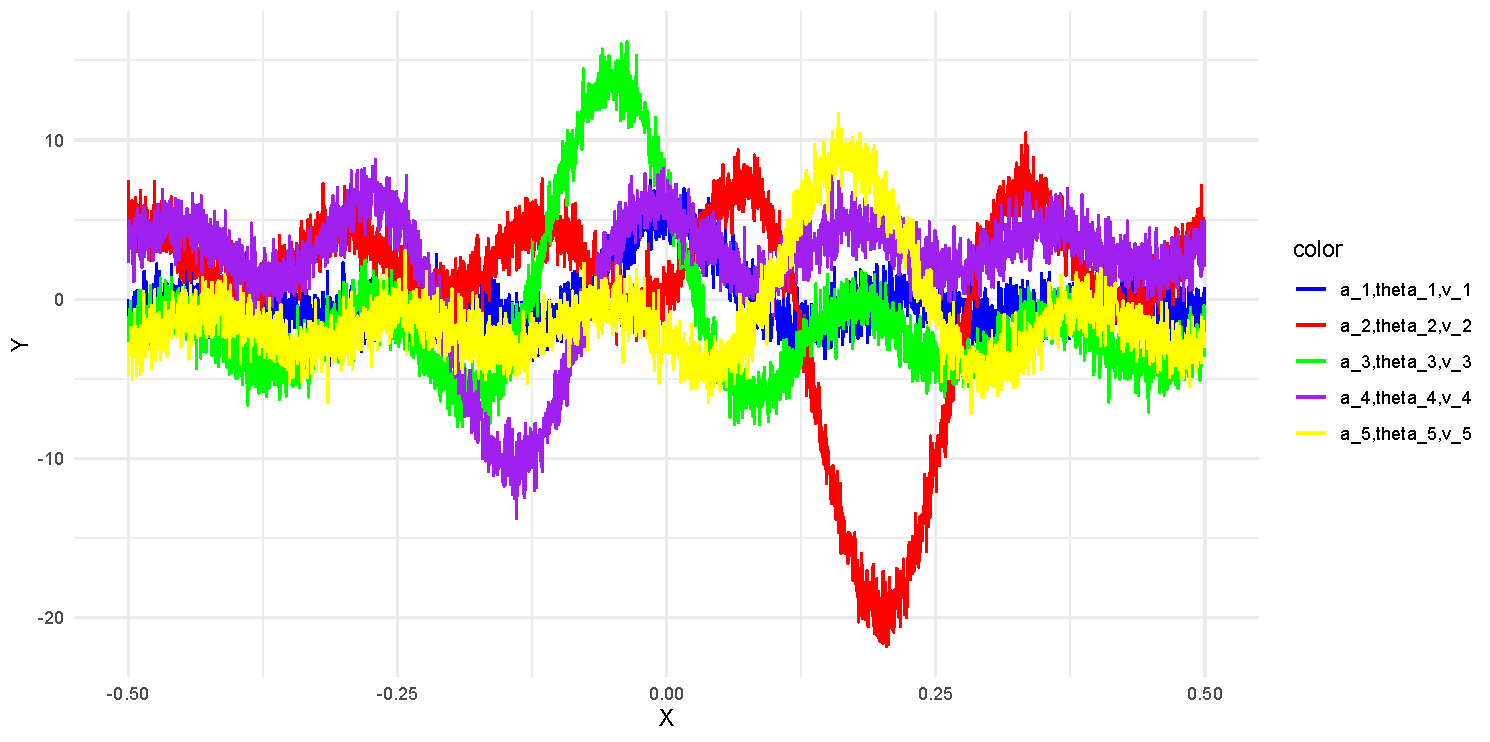
\includegraphics[width=0.65\textwidth]{Mau SP NCKH/image/Stimulated_data_vector_image.pdf}
  \caption{Dữ liệu mô phỏng}
  \label{simulatedata}
\end{figure}

\begin{figure}[ht]
  \centering
  \begin{subfigure}[b]{0.45\textwidth}
    \centering
    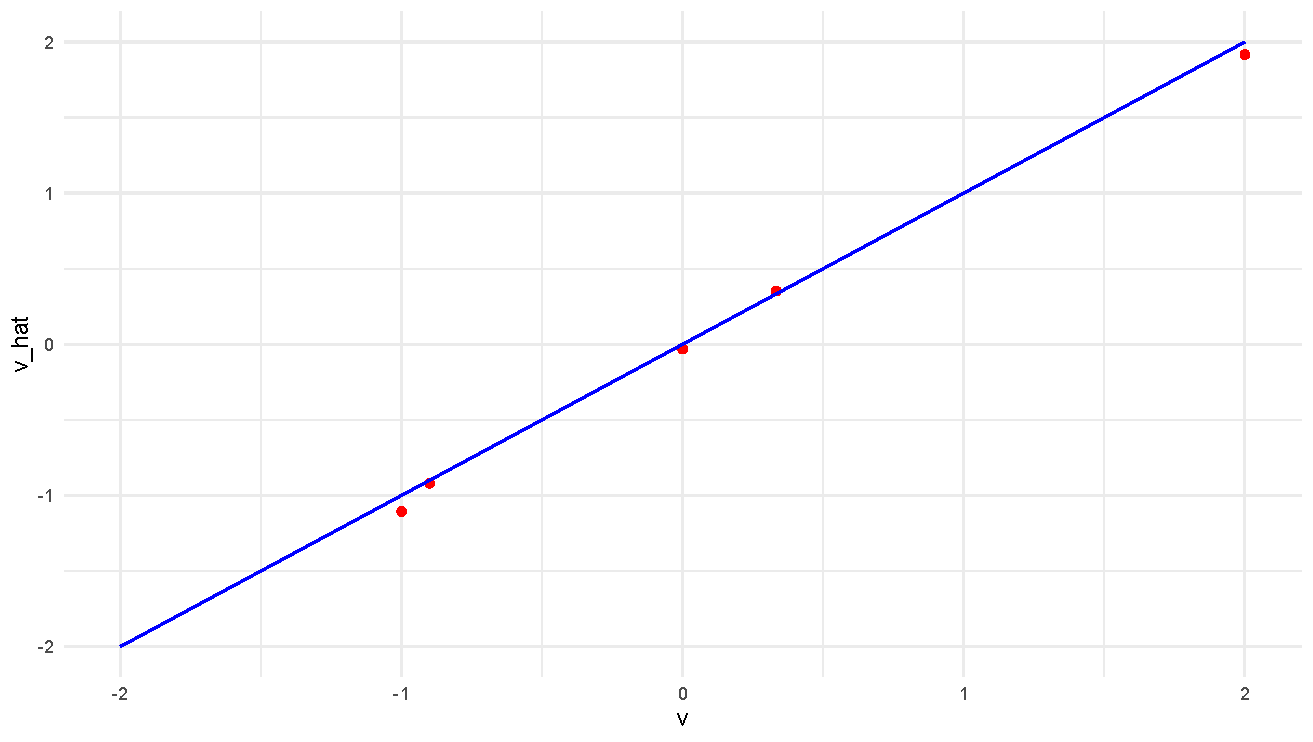
\includegraphics[width=0.8\textwidth]{Mau SP NCKH/image/Approx_v_with_v_nhat2000.pdf}
    \caption{Tham số chiều cao $v$}
    \label{fig:image3}
  \end{subfigure}
  \hfill % optional; add some horizontal spacing
  \begin{subfigure}[b]{0.45\textwidth}
    \centering
    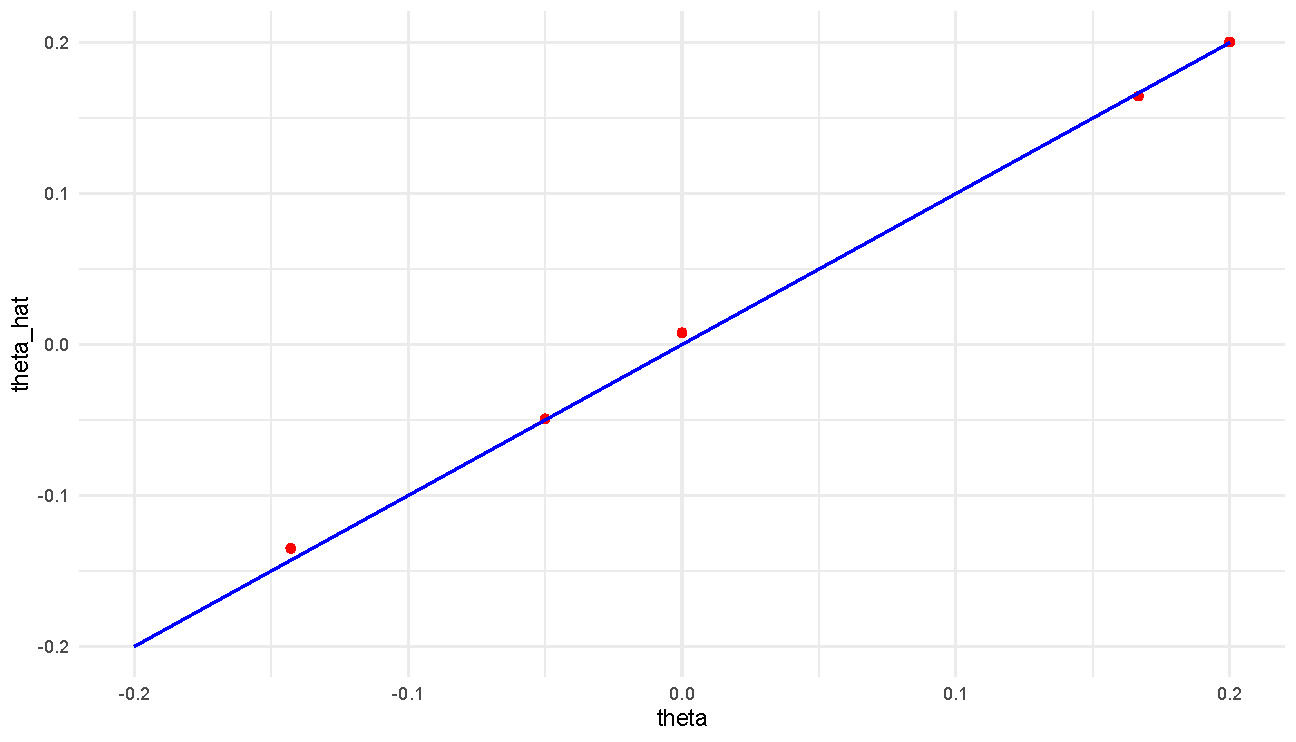
\includegraphics[width=0.8\textwidth]{Mau SP NCKH/image/Approx_theta_with_thetahat2000.pdf}
    \caption{Tham số chuyển $\theta$}
    \label{fig:image2}
  \end{subfigure}

      % Second row with one image centered
  \vspace{0.1cm} % Add vertical space between the rows
  \begin{subfigure}[b]{\textwidth}
    \centering
    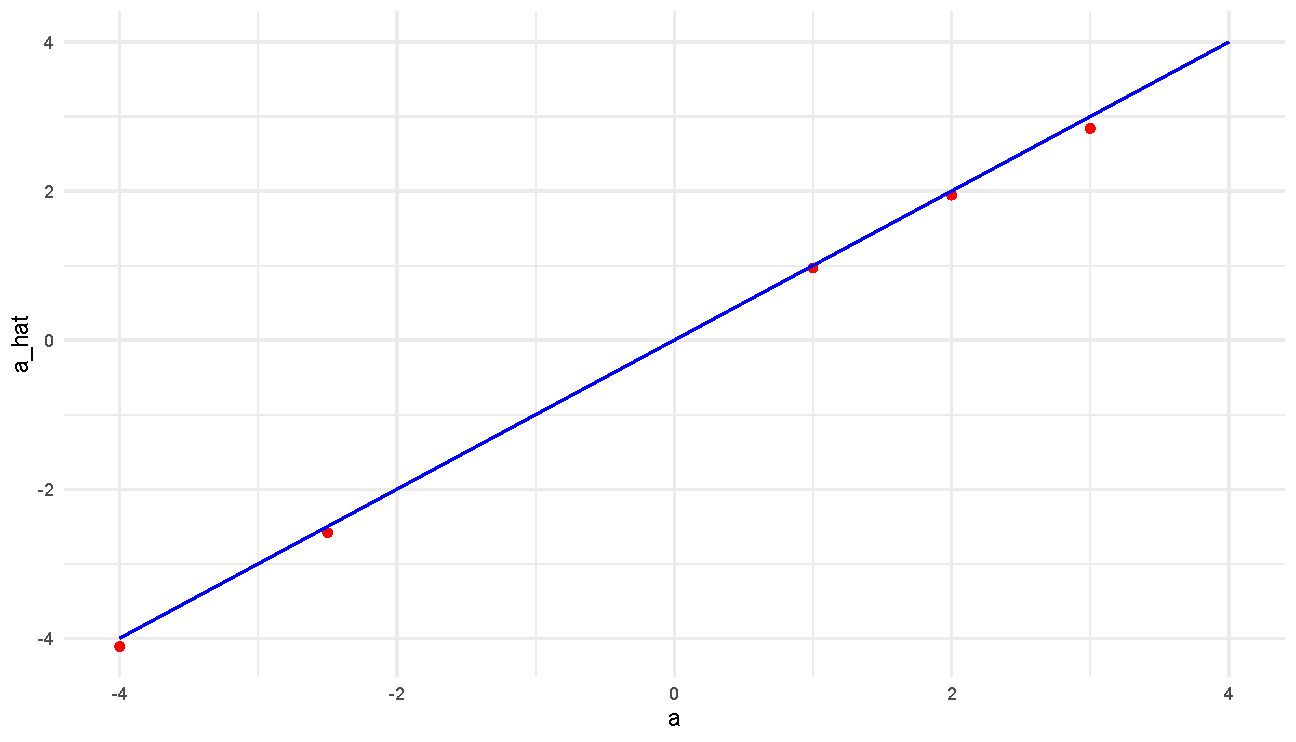
\includegraphics[width=0.4\textwidth]{Mau SP NCKH/image/Approx_a_with_ahat2000.pdf}
    \caption{Tham số co giãn $a$}
    \label{fig:image1}
  \end{subfigure}
  
  \caption{Ước lượng các tham số $v, \theta$ và $a$}
  \label{fig:images-side-by-side}
\end{figure}

\newpage
Hơn nữa, sử dụng sự hội tụ \tref{3.4}, \tref{4.9} và \tref{5.9}, ta có thể nhận được khoảng tin cậy cho các tham số $v, \theta$ và $a$. 
Chẳng hạn, cho $n=2000$, nếu ta đặt $I_{n}\left(v_{2}\right), I_{n}\left(\theta_{3}\right)$ và $I_{n}\left(a_{4}\right)$ là các khoảng tin cậy của $v_{2}, \theta_{1}$ và $a_{1}$, với rủi ro (mức ý nghĩa) $5 \%$, ta có được
$$
\begin{aligned}
I_{n}\left(v_{2}\right) & =[0.243044 ; 0.2920085], \\
\end{aligned}
$$
$$
\begin{aligned}
I_{n}\left(\theta_{1}\right) & =[0.008646117 ; 0.0228825], \\
\end{aligned}
$$
$$
\begin{aligned}
I_{n}\left(a_{1}\right) & =[0.8567415 ;1.005915].
\end{aligned}
$$

Độ dài của các khoảng này lần lượt là $0.0489645,0.01423639$ và 0.1491732. Kết quả là, độ dài của $I_{n}\left(v_{2}\right), I_{n}\left(\theta_{3}\right)$ và $I_{n}\left(a_{4}\right)$ thì nhỏ, nên xác thực khả năng hoạt động hiệu quả của quy trình ước lượng tham số. Tất cả các khoảng tin cậy này được vẽ trong \ref{convergence}.
% \includegraphics[max width=\textwidth, center]{2023_11_01_10532057ac1e795c558bg-15}
\begin{figure}[ht]
  \centering
  \begin{subfigure}[b]{0.45\textwidth}
    \centering
    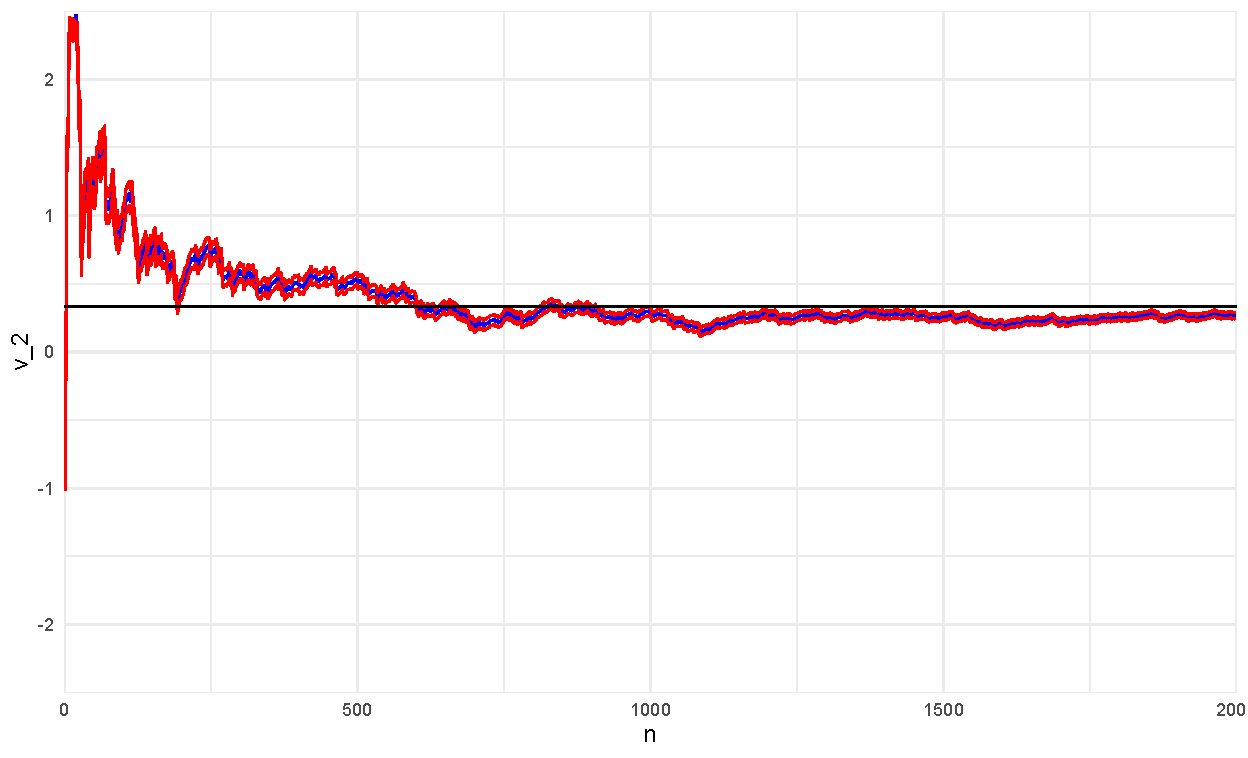
\includegraphics[width=0.8\textwidth]{Mau SP NCKH/image/Convergence/convergence_v_2with_n2000.pdf}
    \caption{Khoảng tin cậy của $v_2$}
    \label{convergence_and_confidence_of_v_1}
  \end{subfigure}
  \hfill % optional; add some horizontal spacing
  \begin{subfigure}[b]{0.45\textwidth}
    \centering
    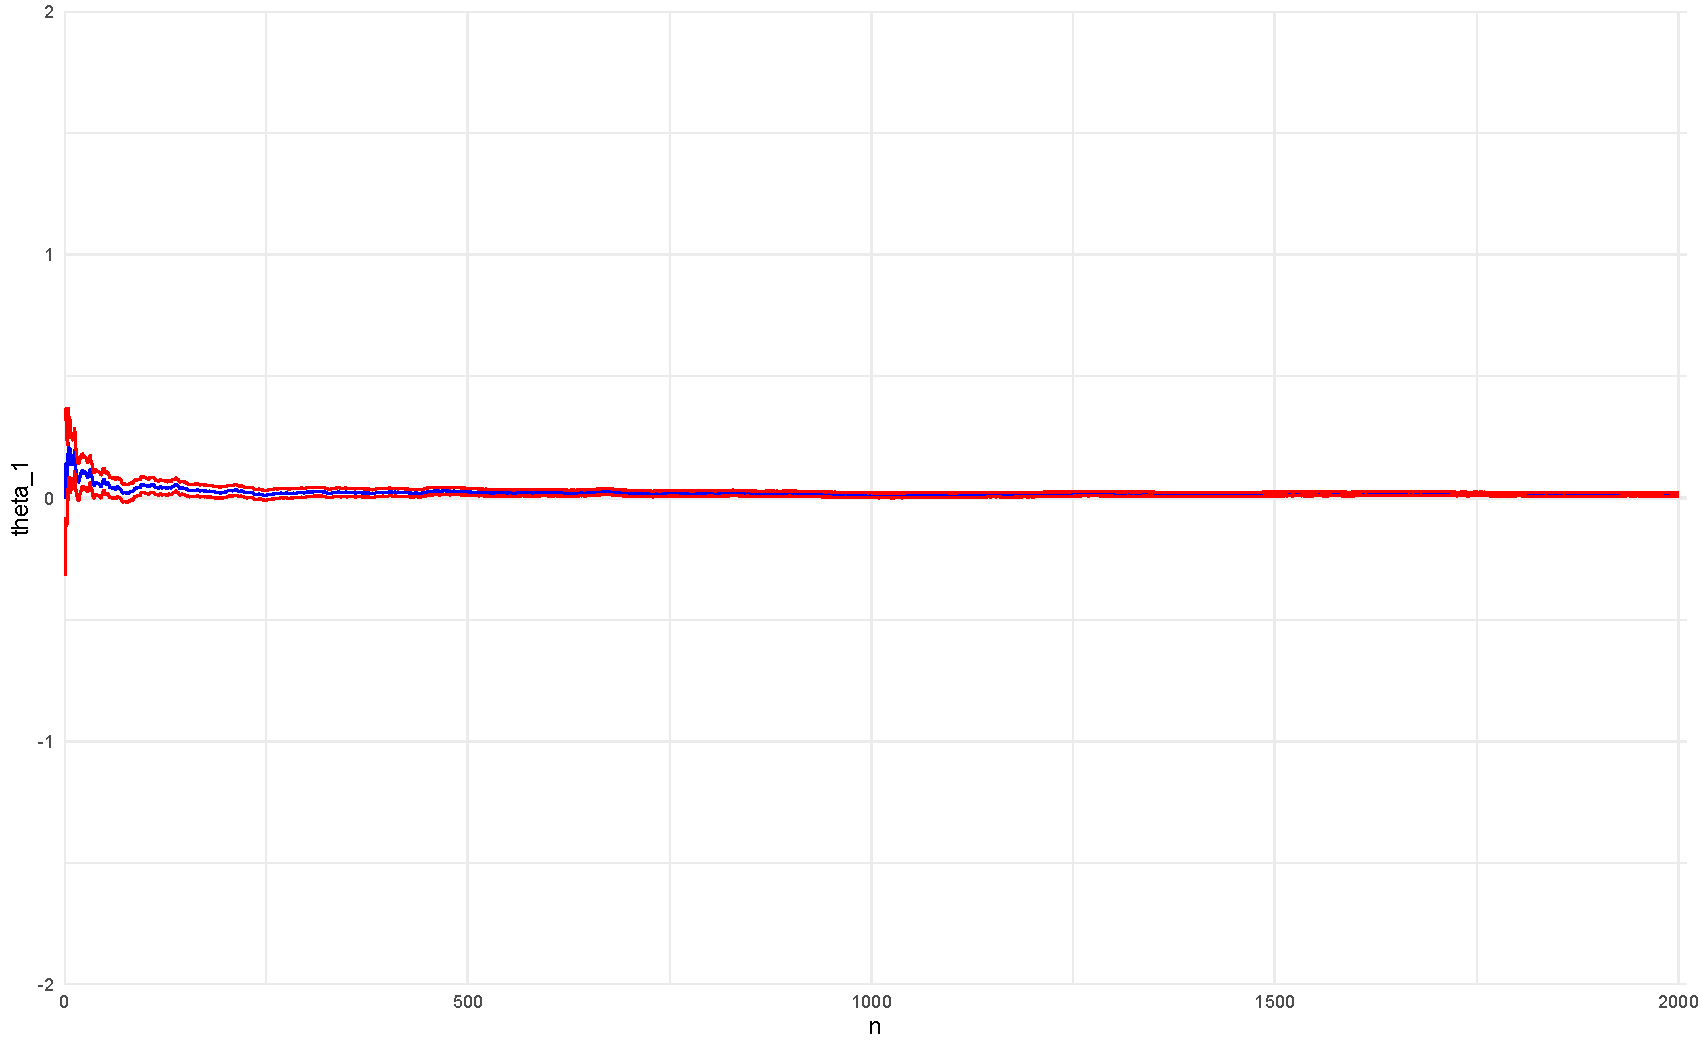
\includegraphics[width=0.8\textwidth]{Mau SP NCKH/image/Convergence/convergence_theta_1with_n2000.pdf}
    \caption{Khoảng tin cậy của $\theta_1$}
    \label{convergence_and_confidence_of_theta_1}
  \end{subfigure}

      % Second row with one image centered
  \vspace{0.1cm} % Add vertical space between the rows
  \begin{subfigure}[b]{\textwidth}
    \centering
    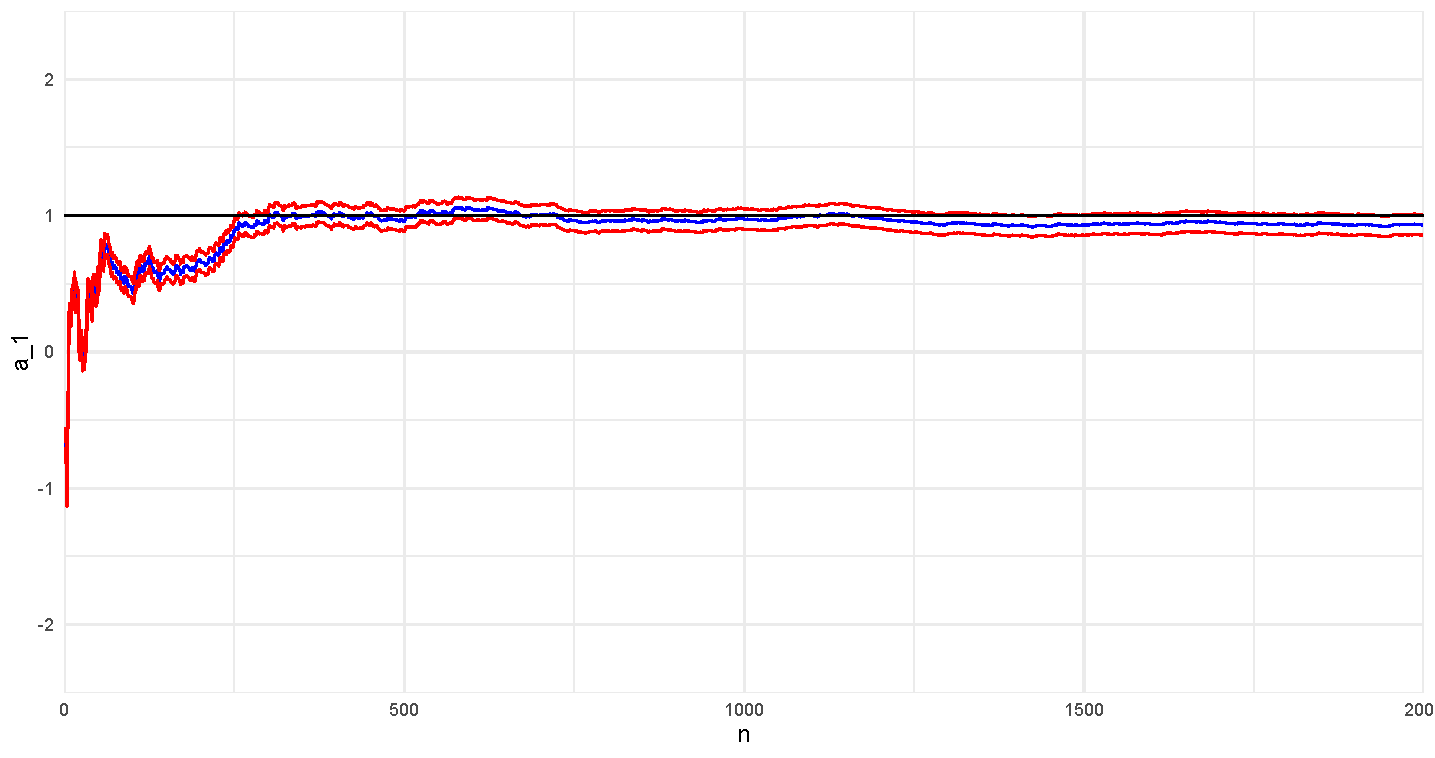
\includegraphics[width=0.4\textwidth]{Mau SP NCKH/image/Convergence/convergence_a_1with_n2000.pdf}
    \caption{Khoảng tin cậy của $a_1$}
    \label{convergence_and_confidence_ofa_1}
  \end{subfigure}
  
  \caption{Khoảng tin cậy của $v_2, \theta_1$ và $a_1$}
  \label{convergence}
\end{figure}


Đối với việc ước lượng hàm hồi quy $f$, ta chọn $\alpha=9 / 10$ cho dãy băng tần $\left(h_{n}\right)$, hàm hạt nhân $K$ sử dụng là hàm hạt nhân đều trên $[-1 ; 1]$ và với mọi $1 \leq j \leq p, \omega_{j}(x)=1 / p$. Việc ước lượng hàm hồi quy $f$ bởi $\widehat{f}_{n}$ được minh họa ở hình bên trái trong hình \ref{convergence_f} , và ước lượng của hàm $f$ bởi $\widehat{f}_{n, 1}$ được minh họa trong hình bên dưới.
\begin{figure}[ht]
  \centering
  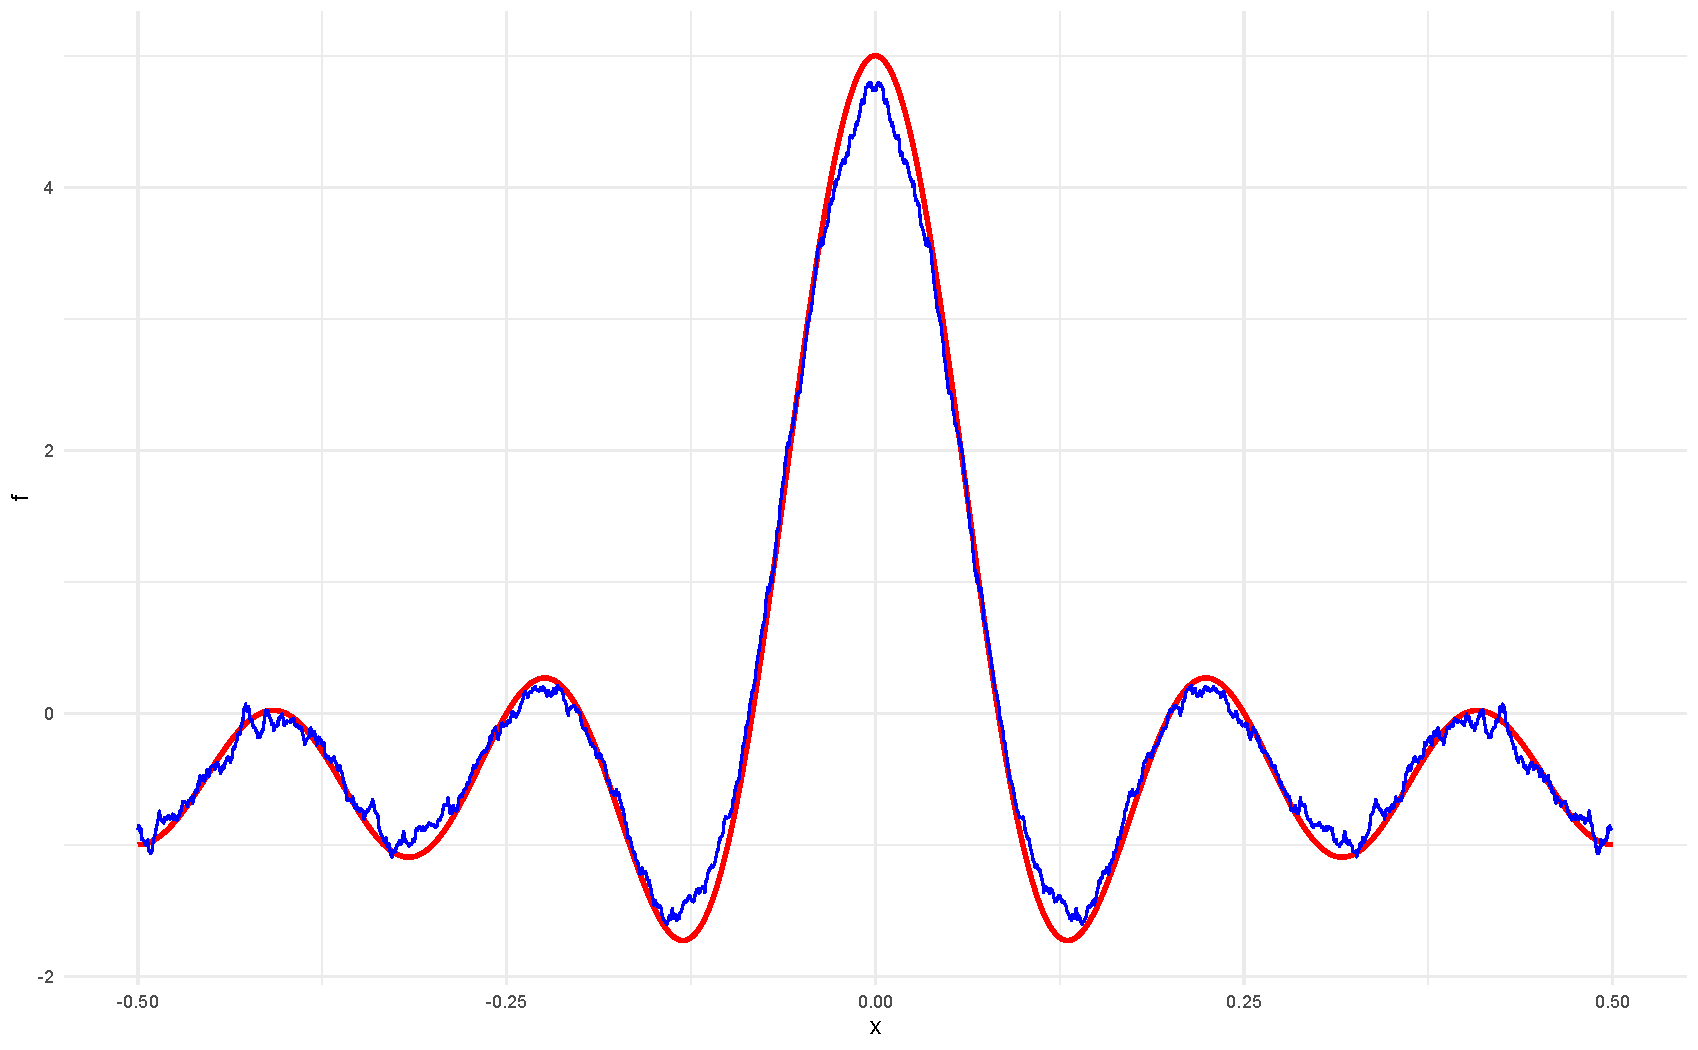
\includegraphics[width=0.65\textwidth]{Mau SP NCKH/image/convergence_f.pdf}
  \caption{Ước lượng hàm $f$ bởi $\hat{f}_n$}
  \label{convergence_f}
\end{figure}
\section{Chương trình R}
Chương trình R để ước lượng các vector tham số $v, \theta, a$  và hàm hồi quy $f$ chia làm sáu phần. Đầu tiên là phần định nghĩa các hàm được sử dụng trong chương trình, sau đó ta sẽ khởi tạo dữ liệu mô phỏng được định nghĩa ở mục trước, tiếp đến lần lượt là các phần chương trình để ước lượng các vector tham số $v, \theta, a$ và phần chương trình cuối cùng - phần thứ sáu sẽ ước lượng hàm hồi quy $f$
\begin{lstlisting}[language=R, title = Phần 1: Các hàm sử dụng trong chương trình]
##########
### Chuan bi cac ham su dung trong chuong trinh
library(ggplot2)
library(ICSNP)
set.seed(45)  # Thiet lap seed de tai tao ket qua
T.test <- function(X, mu=0){
  X <- as.matrix(X)
  n <- nrow(X)
  p <- ncol(X)
  df2 <- n - p
  if(df2 < 1L) stop("Need nrow(X) > ncol(X).")
  if(length(mu) != p) mu <- rep(mu[1], p)
  xbar <- colMeans(X)
  S <- cov(X)
  T2 <- n * t(xbar - mu) %*% solve(S) %*% (xbar - mu)
  Fstat <- T2 / (p * (n-1) / df2)
  pval <- 1 - pf(Fstat, df1=p, df2=df2)
  data.frame(T2=as.numeric(T2), Fstat=as.numeric(Fstat),
             df1=p, df2=df2, p.value=as.numeric(pval), row.names="")
}


T.ci <- function(mu, Sigma, n, avec=rep(1,length(mu)), level=0.95){
  p <- length(mu)
  if(nrow(Sigma)!=p) stop("Need length(mu) == nrow(Sigma).")
  if(ncol(Sigma)!=p) stop("Need length(mu) == ncol(Sigma).")
  if(length(avec)!=p) stop("Need length(mu) == length(avec).")
  if(level <=0 | level >= 1) stop("Need 0 < level < 1.")
  cval <- qf(level, p, n-p) * p * (n-1) / (n-p)
  zhat <- crossprod(avec, mu)
  zvar <- crossprod(avec, Sigma %*% avec) / n
  const <- sqrt(cval * zvar)
  c(lower = zhat - const, upper = zhat + const)
}


rma <- function(x, p, r = TRUE){
  # Mo rong ma tran theo hang va cot
  # matrix                  x: ma tran dau vao
  # line of extend          p: So dong muon mo rong
  # direction of extension  r: TRUE neu mo rong theo hang, FALSE neu mo rong theo cot
  # state: da kiem tra ham nay la dung
  c_or_r = x
  if(r == TRUE){
    for(i in 2:p){
      x = rbind(x,c_or_r)
    }
  }else{
    for(i in 2:p){
      x = cbind(x,c_or_r)
    }
  }
  return(x)
}


sum_broadcast <- function(a,b){
  # a va b lan luot tuong ung voi ma tran co so chieu dim (p,1) and (1,p)
  return(rma(a,dim(b)[2],r=FALSE)+rma(b,dim(a)[1]))
}


D <- function(X,t,p=5){
  # state: da kiem tra ham nay la dung
  # input X: mot bien ngau nhien, EX: X[1,1]
  g = 1
  t = matrix(t,nrow=length(t), ncol=1)
  s = (1/g)*c(sin(2*pi*(X-t[1,])))
  for(i in 2:p){
    s = c(s,(1/g)*sin(2*pi*(X-t[i,])))
  }
  return(diag(s))
}


my_f <- function(x) {    
  out <- cos(2*pi*(x))*(cos(2*pi*1*(x)) + cos(2*pi*2*(x)) + cos(2*pi*3*(x)) + cos(2*pi*4*(x)) + cos(2*pi*5*(x)))
  return(out)
}


f1 <- integrate(my_f,          # Ap dung tinh tich phan trong R
                lower = -1/2,
                upper = 1/2)


f <- function(x){
  out2 <- cos(2*pi*1*(x))+cos(2*pi*2*(x))+cos(2*pi*3*(x))+cos(2*pi*4*(x))+cos(2*pi*5*(x))
  return(out2)
}

Vectorize_f <- Vectorize(f)
\end{lstlisting}

\begin{lstlisting}[language=R, title = Phần 2: Tạo dữ liệu mô phỏng]
p =  5
n = 2000
g = 1
rowx <- runif(n, min=-0.5,max= 0.5)  # Tao gia tri x
x = matrix(rowx,nrow = 1,ncol = length(rowx))
x = rma(x,p=p)

# Chuan bi cac vecto v, theta, a and esp
v = matrix(c(0,1/3,-1,2,-9/10),nrow=p,ncol=1)
theta = matrix(c(0,1/5,-1/20,-1/7,1/6),nrow=p,ncol=1)
a = matrix(c(1,-4,3,-5/2,2),nrow=p,ncol=1)


##
f_vec <- Vectorize(f)
gamma_j <-  1/(2*pi*a*(1/2))
##

esp = matrix(rnorm(n*p, mean = 0, sd = 1), nrow=p)
Y = (rma(a, n, r= FALSE))*f_vec(x-rma(theta,n,r=FALSE)) + rma(v,n, r=FALSE) + esp

# Khi ma bind xong thi Y la matrix

# dataframe
df <- data.frame(
  x = c(t(x)),
  y = c(t(Y)),
  wave = factor(c(rep('a_1,theta_1,v_1', n),
                  rep('a_2,theta_2,v_2', n),
                  rep('a_3,theta_3,v_3', n),
                  rep('a_4,theta_4,v_4', n),
                  rep('a_5,theta_5,v_5', n))))

# Tao cac bieu do duong
ggplot(df, aes(x = x, y = y, color = wave)) + 
  geom_line() +  # Them cac lop chi tiet cho bieu do
  xlab('x') +
  ylab('y') +
  theme_minimal() +
  scale_color_manual(values = c('blue', 'red', 'green', 'purple', 'yellow'))
\end{lstlisting}
Ước lượng tham số chiều cao $v$
\begin{lstlisting}[language=R, title = Phần 3: Ước lượng tham số chiều cao]
##################################################
# Uoc luong tham so chuyen v
# Tinh v_n
v_n = matrix(diag(diag(p))-0.75, nrow=p, ncol=1)
cv = 0
for(i in 2:n){
  cv <- 0
  for(j in 1:i){
    cv <- cv + (1/i)*Y[,j]/g  # This calculates average per row
  }
  v_n <- cbind(v_n, (cv))  
}
\end{lstlisting}
\begin{lstlisting}[language=R,title = Phần 4: Ước lượng tham số chuyển]
##################################
# Estimate theta parameters
f1_hat <- function(x,Y,n, g = 1){
  # x is vector EX: x[1,]
  # y is vector EX: Y[1,]
  x = matrix(x,nrow = 1)
  Y = matrix(Y,ncol = 1)
  return((1/n)*((cos(2*pi*x)/g)%*%Y))
}

# f1_hat = (1/n)*matrix(cos(2*pi*x[1,]),nrow = 1)%*%matrix(Y[1,],nrow = length(Y[1,]))  

C <- function(X,t,p=5){
  g = 1
  t = matrix(t,nrow=length(t), ncol=1)
  s = (1/g)*c(cos(2*pi*(X-t[1,])))
  for(i in 2:p){
    s = c(s,(1/g)*cos(2*pi*(X-t[i,])))
  }
  return(diag(s))
}
# Estimate theta
pi_K <- function(x) {
  #state: checked
  ifelse(abs(x) <= 1/4, x, ifelse(x > 1/4, 1/4, -1/4))
}
pi_K_vectorized <- Vectorize(pi_K) # Tra ve mot day so co tri tuyet doi nho hon hoac bang 0.25

N = n
gamma <- 1/ (1:n)  
theta_hat = c(0,0,0,0,0)
matrix_theta =  matrix(theta_hat, ncol=1)

# Uoc luong theta
for (nn in 1:(N-1)) { #(N-1)
  T_np <- D(x[1,nn+1],theta_hat)%*%matrix(Y[,nn+1],nrow=p,ncol=1) # Assuming Y_n = 1 and g(X_n) = 1 (uniform density)
  index = nn + 1
  theta_hat <- pi_K_vectorized(matrix(theta_hat,nrow=p,ncol=1) + (gamma_j*gamma[index]) * T_np)
  matrix_theta = cbind(matrix_theta, theta_hat)
}
\end{lstlisting}
\newpage
\begin{lstlisting}[language=R, title = Phần 5: Ước lượng tham số co giãn]
###############################################################################
# Uoc luong asim
C <- function(X,t,p=5){
  g = 1
  t = matrix(t,nrow=length(t), ncol=1)
  s = (1/g)*c(cos(2*pi*(X[1,]-t[1,])))
  if(p >= 2){
    for(i in 2:p){
      s = c(s,(1/g)*cos(2*pi*(X[i,]-t[i,])))
    }  
  }
  return(diag(s))
}

vector_asim = (1/(2*f1$value))*diag(C(matrix(x[1,2:2],ncol=1), matrix_theta[1,1:(2-1)],p=2-1))%*%matrix(Y[1,2:2],ncol = 1)
matrix_asim = matrix(0, nrow = 1, ncol = n - 2)
for(j in 1:p){
  for(i in 3:n){
    asim_i = (1/(i*f1$value)*diag(C(matrix(x[1,2:i],ncol=1), matrix_theta[j,1:(i-1)],p=i-1))%*%matrix(Y[j,2:i],ncol = 1))
    vector_asim = c(vector_asim, asim_i)
  }
  matrix_asim <- rbind(matrix_asim, matrix(vector_asim,nrow = 1))
  vector_asim = (1/(2*f1$value))*diag(C(matrix(x[1,2:2],ncol=1), matrix_theta[j,1:(2-1)],p=2-1))%*%matrix(Y[j,2:2],ncol = 1)
}
matrix_asim = matrix_asim[2:dim(matrix_asim)[1], ]
last_col <- matrix(matrix_asim[,n-(n - dim(matrix_asim)[2] + 1)], ncol = 1)
for(i in 1:(n - dim(matrix_asim)[2])){
  matrix_asim <- cbind(matrix_asim, last_col)
}
\end{lstlisting}
\begin{lstlisting}[language=R, title = Phần 6: Ước lượng hàm hồi quy $f$ và vẽ hình minh họa]
###########################################################################
# Da chuan bi xong v_n, matrix_theta, matrix_asim
# Tien hanh uoc luong ham hoi quy f
fn_hat <- function(x, kernel, n = 1500){
  weight = diag(1/p*diag(1,p,p))
  alpha = 9/10
  x = matrix(x,nrow = 1, ncol = n)
  
  
  
  # uniform_kernel_vectorized return sequence c()
  h = matrix(c(1:n), nrow = 1)**alpha
  xn = matrix(x[,1:n], nrow = 1)
  for(j in 1:p){
    thetan_j = matrix(matrix_theta[j,1:n], nrow = 1)
    xn = xn - thetan_j - x
    inpK = (1/h)*xn
  }  
}

uniform_kernel <- function(u) {
  # Ap dung ham hat nhan deu
  # K(u) = 1/2 if |u| <= 1, neu khong thi K(u) = 0
  ifelse(abs(u) <= 2, 1/4, 0)
}

uniform_kernel_vectorized <- Vectorize(uniform_kernel)

gaussian_kernel <- function(u) {
  # Ham hat nhan Gauss
  1 / sqrt(2 * pi) * exp(-u^2 / 2)
}

gaussian_kernel_vectorized <- Vectorize(gaussian_kernel)

inpK <- function(xn, theta, x, h){
  # Kiem soat input dau vao
  xn = matrix(xn, nrow = 1)
  theta = matrix(theta, nrow = 1)
  x = matrix(x, nrow = 1)
  h = matrix(h, nrow = 1)
  
  xn = xn - theta - x
  inpK = (1/h)*xn
  return(inpK)
}
# uniform_kernel_vectorized tra ve mot day seq()
weight = matrix(diag(1/p*diag(1,p,p)), nrow = 1)
alpha = 9/10
matrix_fn_hat = seq()
nopoint = 2000
for(i in 3:nopoint){
  h = (1/matrix(c(1:n), nrow = 1, ncol = n))**alpha
  xn = matrix(x[1,1:n], nrow = 1)
  x1 = matrix(seq(-0.5,0.5, length.out = nopoint)[i],nrow = 1, ncol = n) 
  matrix_fn_hat_j = seq()
  for(j in 1:p){
    thetan_j = matrix(c(matrix_theta[j,1],matrix_theta[j,1:n-1]), nrow = 1, ncol = n)
    inpKp = inpK(xn, thetan_j,  x1, h)
    inpKm = inpK(xn, thetan_j, -x1, h)
    matrixKp = matrix(uniform_kernel_vectorized(inpKp),nrow = 1)
    matrixKm = matrix(uniform_kernel_vectorized(inpKm),nrow = 1)
    Swp = (1/h)*matrixKp
    Swm = (1/h)*matrixKm
    Sw = (Swp + Swm)
    
    fsim_j = matrix(Y[j,1:n],ncol = 1) - matrix(c(v_n[j,1],v_n[j,1:n-1]), ncol = 1)
    
    fn_hat_j = (1/matrix_asim[j,n])*(Sw%*%fsim_j)/sum(Sw)
    matrix_fn_hat_j = c(matrix_fn_hat_j, fn_hat_j[1])
  }
  fn_hat = weight%*%matrix(matrix_fn_hat_j[2:length(matrix_fn_hat_j)], ncol = 1, nrow = length(matrix_fn_hat_j[2:length(matrix_fn_hat_j)]))
  matrix_fn_hat = c(matrix_fn_hat, fn_hat)
}
  
#############################################################################
# dataframe
df <- data.frame(
  x = c(seq(-0.5,0.5, length.out=nopoint-1)),
  y = c(matrix(matrix_fn_hat[2:n],ncol = 1, nrow = n-1)))
  y_true = Vectorize_f(c(seq(-0.5,0.5, length.out=nopoint-1)))


# Ve bieu do hoi tu cua uoc luong f_hat_n ve ham f
ggplot() +  
  geom_line(data = df, aes(x = x, y = y_true), color = 'red', size = 1)+
  geom_line(data = df, aes(x = x, y = y), color = 'blue')+   # Them cac chi tiet cho bieu do
  xlab('x') +
  ylab('f') +
  theme_minimal() +
  scale_color_manual(values = c('blue', 'red', 'green', 'purple', 'green'))



\end{lstlisting}
%Hơn nữa, theo sự hội tụ \tref{6.6} và \tref{6.7}, cho $n=2000$ và với mọi $x \in[-1 / 2 ; 1 / 2]$, 

%Ta có sự hội tụ của hàm $\widehat{f}_n$ về $f$ như trong hình 4.4
% khoảng tin cậy của $f(x)$ xác định bởi
% $$
% K_{n}(x)=\left[\widehat{f}_{n}(x)-q_{\beta} \frac{\widehat{w}_{n}\left(x, \widehat{\theta}_{n}\right)}{\sqrt{n h_{n}}}, \widehat{f}_{n}(x)+q_{\beta} \frac{\widehat{w}_{n}\left(x, \widehat{\theta}_{n}\right)}{\sqrt{n h_{n}}}\right]
% $$
% trong đó ta có thể suy ra từ sự hội tụ \tref{3.3} và \tref{3.4} của Định lý 3.2 trong \cite{bercu} rằng cho $n=2000$ và với mọi $x \in[-1 / 2 ; 1 / 2]$, một khoảng tin cậy cho hàm $f(x)$ xác định bởi
% $$
% J_{n}(x)=\left[\widehat{f}_{n, 1}(x)-q_{\beta} \frac{\widehat{v}_{n}\left(x, \widehat{\theta}_{n, 1}\right)}{\sqrt{n h_{n}}}, \widehat{f}_{n, 1}(x)+q_{\beta} \frac{\widehat{v}_{n}\left(x, \widehat{\theta}_{n, 1}\right)}{\sqrt{n h_{n}}}\right]
% $$
% trong đó $q_{\beta}$ phân vị cấp $0<\beta<1$ của phân phối $\mathcal{N}(0,1)$ và $\widehat{w}_{n}^{2}\left(x, \widehat{\theta}_{n}\right)$ và $\widehat{v}_{n}^{2}\left(x, \widehat{\theta}_{n, 1}\right)$ là một ước lượng vững của phương sai tiệm cận của $w^{2}(x, \theta)$ trong Định lý 6.2 và của $v^{2}\left(x, \theta_{1}\right)$ trong Định lý 3.2 của \cite{bercu}. Trong trường hợp này $\nu^{2}=1 / 2$, và một tính toán số học dẫn đến
% $$
% w^{2}(x, \theta)= \begin{cases}0.0114 & \text { nếu }-1 / 2 \leq x \leq-23 / 50 \text { và } 23 / 50 \leq x \leq 1 / 2, \\ 0.0108 & \text { nếu }-23 / 50<x \leq-9 / 25 \text { và } 9 / 25 \leq x<23 / 50 \\ 0.0099 & \text { nếu }-9 / 25<x \leq-17 / 50 \text { và } 17 / 50 \leq x<9 / 25 \\ 0.0086 & \text { nếu }-17 / 50<x \leq-31 / 100 \text { và } 31 / 100 \leq x<17 / 50, \\ 0.0083 & \text { nếu }-31 / 100<x<0 \text { và } 0<x<31 / 100, \\ 0.0166 & \text { nếu } x=0,\end{cases}
% $$
% và
% $$
% v^{2}\left(x, \theta_{1}\right)= \begin{cases}5 / 38 & \text { nếu } x \neq 0 \\ 5 / 19 & \text { nếu } x=0\end{cases}
% $$
% Nói cách khác, với mọi $x \in[-1 / 2 ; 1 / 2]$, bậc của phương sai tiệm cận $v^{2}\left(x, \theta_{1}\right)$ nhận được từ ước lượng $\widehat{f}_{n, 1}$ gấp hơn mười lần so với bậc của phương sai tiệm cận $w^{2}(x, \theta)$ nhận được từ $\widehat{f}_{n}$. Thêm vào đó, trong trường hợp này, phương sai tối đa được cho trong Chú ý 6.2 là, với mọi $x \in[-1 / 2 ; 1 / 2]$, có bậc $10^{-3}$ nhỏ hơn $w^{2}(x, \theta)$ mười lần. Các khoảng tin cậy $K_{n}(x)$ và $J_{n}(x)$ được vẽ bằng màu đỏ trong Figure 5. Ta có thể thấy trong Figure 4 rằng ước lượng $\widehat{f}_{n}$ thì gần hàm $f$ hơn $\widehat{f}_{n, 1}$. Chính xác hơn, ước lượng của hàm $f$ bởi $\widehat{f}_{n}$ thì tốt hơn ước lượng bởi $\widehat{f}_{n, 1}$ vì độ dài khoảng tin cậy $K_{n}(x)$ thì nhỏ hơn độ dài $J_{n}(x)$ như có thể thấy được trong Figure 5, tùy thuộc vào bậc của hai phương sai $v^{2}\left(x, \theta_{1}\right)$ và $w^{2}(x, \theta)$. Trong trường hợp của ta,  khoảng tin cậy lớn nhất $K_{n}(x)$ có độ dài 0.3460 (khi $x=0$ ) và nhỏ hơn gần ba lần so với $J_{n}(x) = 0.9723$ (khi $x=-0.09$ và $x=0.09)$. Cụ thể hơn, điều này khẳng định lựa chọn phiên bản ước lượng Nadaraya-Watson có trọng.
% %\includegraphics[max width=\textwidth, center]{2023_11_01_10532057ac1e795c558bg-17(1)}

% Figure 4 . Ước lượng hàm $f$ bởi $\widehat{f}_{n}$ và $\widehat{f}_{n, 1}$
% %\includegraphics[max width=\textwidth, center]{2023_11_01_10532057ac1e795c558bg-17}

% Figure 5. Các khoảng tin cậy của hàm $f$



% \subsection{Nội dung xây dựng thuật toán}
% Tôi xem xét
% \verb|x| là một ma trận p dòng và n cột, $\mathbf{x} \in \mathbb{R}^{p\times n}$
% \verb|x| là một ma trận p dòng và n cột, $\mathbf{x} \in \mathbb{R}^{p\times n}$

\chapter*{Kết luận}
Trong khóa luận này, tôi đã trình bày chứng minh các kết quả liên quan đến mô hình biến dạng có chu kỳ \tref{1.1} bao gồm sự hội tụ của các ước lượng tham số và phi tham số, còn có các kết quả về tính tiệm cận chuẩn, luật loga-lặp và luật mạnh dạng toàn phương. Việc ứng dụng các kết quả đó để xây dựng thuật toán và viết chương trình chạy trên dữ liệu mô phỏng đem đến những kết quả tốt, chứng tỏ phương pháp thực sự hiệu quả trên dữ liệu mô phỏng, đồng thời các biểu hiện tích cực đó của phương pháp mở ra những hy vọng về sự hiệu quả khi ứng dụng phương pháp trên cho các dữ liệu thực tế.

Các công việc tiếp theo cần phải làm là xây dựng thêm các lý thuyết để loại bỏ việc sử dụng dấu của $a$ và hệ số Fourier thứ nhất của hàm $f$, làm nền tảng để ứng dụng phương pháp trên cho các dữ liệu tuần hoàn trong thực tế mà tiêu biểu là dữ liệu điện tim. Đó cũng chính là các nội dung tôi mong muốn làm được sau khi kết thúc khóa luận.

Qua việc thực hiện khóa luận, tôi đã học thêm được rất nhiều kiến thức về lĩnh vực "Xác suất phi tuyến" như là các định lý "Luật số lớn", "Định lý giới hạn trung tâm" cho những đối tượng toán học khác nhau. Một số lý thuyết đời thường mà thú vị về trò chơi công bằng - xuất phát điểm của lý thuyết martingale,... . Mặc dù, việc nghiên cứu nhiều lần làm tôi mệt, nhưng hành trình này cũng mang đến sự vui vẻ trong tâm thức mà qua đó dìu dắt tôi hoàn thành trọn vẹn khóa luận này. Tôi không đặt kỳ vọng các bạn sinh viên Toán lứa sau sẽ làm khóa luận, song vẫn động viên các bạn lăn xả nếu có thể. Vì lý do gì nào? Tôi hy vọng các bạn có thể tự tìm ra cho mình.

Một lần nữa, xin gửi lời cảm ơn chân thành đến thầy Nguyễn Phát Đạt, vì đã cho phép và hỗ trợ tôi từ lúc bắt đầu đến khi kết thúc khóa luận này. Cảm ơn sự gần gũi như một người anh của thầy, những sự động viên của thầy đã giúp em dũng cảm hơn rất nhiều để đối mặt với những khó khăn tri thức khi thực hiện đề tài này. Cảm ơn thầy... rất nhiều.
%\chapter*{Phụ lục}


\addcontentsline{toc}{chapter}{Tài liệu tham khảo}
\begin{thebibliography}{9}

\bibitem{fraysse1} Fraysse, P. (2014). {\em Recursive Estimation in a Class of Models of Deformation, Journal of Statistical Planning and Inference}, 132-158.
	
\bibitem{bercu} Bercu, B. and Fraysse, P. (2012). {\em A Robbins-Monro Procedure for Estimation in Semiparametric Regression Models}.

\bibitem{duflo} Duflo, M. (1997). {\em Random Iterative Models. Applications of Mathematics(New York)}, Springer, Berlin.

\bibitem{bercuslide} Bercu, B. (2014). {\em Asymptotic Results for Martingales with Statistical applications}.

\bibitem{kushner} Kushner, H.J and Yin, G.G (2003). {\em Stochastic Approximation and Recursive Algorithms and Applications}. Applications of Mathematics(New York), Springer.

\bibitem{bruce} Bruce M. Brown (1971). {\em Martingale Central Limit Theorems}.

\bibitem{chaabane} Chaabane, F. and Maaouia, F. (2000). {\em Théorèmes Limites Avec Poids Pour Les Martingales Vectorielles}, ESAIM PS, 4, 137–189.

\bibitem{tien} Tiến, N.D. (2001). {\em Các mô hình xác suất và ứng dụng. Phần III, giải tích ngẫu nhiên}, NXB Đại học Quốc gia Hà Nội, 44-47.

\bibitem{pelletier_on_the_almost} Pelletier, M. (1998). {\em On The Almost Sure Asymtotic Behavior of Stochastic algorithms}.

\bibitem{pelletier_weak_convergence} Pelletier, M. (1998).{\em Weak convergence rates for stochastic approximation with application to multiple targets and simulated annealing}. Annals of Appli. Proba. 8, 1, 10-44.

\bibitem{nguyen_thanh_nhan} Trần Minh Phương, Nguyễn Thành Nhân (2022), {\em Giải tích số và ứng dụng (phần cơ bản)}, NXB Đại học Sư phạm TPHCM.

\bibitem{noda} Noda, K. (2007). Estimation of a Regression Function by The Parzen kernel-type Density Estimatiors, Ann Inst Statist Math, 221-234.

\bibitem{schuster} Schuster, E.F. (1972). Joint Asymptotic Distribution of The Esimated Regression Function at a Finite Number of distinct Points, 84-88.

\end{thebibliography}

\newpage
\addcontentsline{toc}{chapter}{\indexname}
\printindex
\end{document}
